\documentclass[paper=a4,11pt]{scrreprt}

\usepackage[utf8]{inputenc}
\usepackage[ngerman]{babel}
\usepackage[T1]{fontenc}	
\usepackage{amsmath}
\usepackage{graphicx}
\usepackage{listings}
\usepackage{pdfpages}

\renewcommand\lstlistingname{Source Code}
\renewcommand\lstlistlistingname{Source Code}

\usepackage{xcolor}
\definecolor{codegreen}{rgb}{0,0.6,0}
\definecolor{codegray}{rgb}{0.5,0.5,0.5}
\definecolor{codeorange}{rgb}{1,0.49,0}
\definecolor{backcolour}{rgb}{0.95,0.95,0.96}
\definecolor{funccolour}{rgb}{0.3, 0.6, 0.9}


\lstdefinestyle{mystyle}{
    backgroundcolor=\color{backcolour},   
    commentstyle=\color{codegray},
    keywordstyle=\color{codeorange},
    numberstyle=\tiny\color{codegray},
    stringstyle=\color{codegreen},
    identifierstyle =\color{funccolour},
    basicstyle=\ttfamily\footnotesize,
    breakatwhitespace=false,         
    breaklines=true,                 
    captionpos=b,                    
    keepspaces=true,                 
    numbers=left,                    
    numbersep=5pt,                  
    showspaces=false,                
    showstringspaces=false,
    showtabs=false,                  
    tabsize=2,
    xleftmargin=10pt,
}
\lstset{style=mystyle}

\title{Technikerprojekt: E-Bike ECU}
\author{Leon Reeh}
\date{\today}

\begin{document}

\maketitle
\paragraph{Vorwort}
Um das Lesen zu vereinfachen, wurde die Dokumentation in vier Teile unterteilt. Diese vier Abschnitte beschäftigen sich jeweils vollständig mit einem Aspekt des Projekts und stehen für sich:\\
\textbf{Teil 1}: Einleitung und Beschreibung des vollständigen Systems.\\ 
\textbf{Teil 2}: Dokumentation des fertigen Schaltplans, Layouts, der Software und Mechanik im Detail. \\
\textbf{Teil 3}: Der Entwicklungsprozess mit Designänderungen und deren Hintergründen.\\ 
\textbf{Teil 4}: Anhänge, einschließlich des vollständigen Schaltplans und Quellausschnitte.\\
\\Die vollständige Dokumentation sowie der vollständige und durchgehend verfügbare Software-Quellcode, Schaltpläne und weitere Dateien stehen ebenfalls in digitaler Form auf GitHub unter \textbf{https://github.com/leonreeh/E-Bike-ECU} zur Verfügung.
\paragraph{Lizenz}
Dieses Projekt und die hier beiliegende dokumentation fallen unter die MIT-Lizenz (X11-Lizenz) \emph{Leon Reeh 2025} 

\tableofcontents
\newpage


\part{Einleitung und Projektbeschreibung}
\chapter{Einleitung}
\textbf{Ziel des Projekts} ist die Entwicklung eines Steuergeräts für einen akkubetriebenen BLDC-Heckmotor mit einer Nennleistung von 1000 W bei 48 V für ein E-Bike. Das Steuergerät soll alle relevanten Bedienelemente für den Motorbetrieb sowie die Steuerung der Beleuchtung integrieren. Die Umsetzung erfolgt mit einer selbst entwickelten Platine auf Mikrocontroller-Basis und einer eigens programmierten Software.
\textbf{Motivation}
Warum habe ich dieses Projekt gewählt? 
Nach zehn Jahren Firmenzugehörigkeit bei Panasonic Lüneburg – einem Unternehmen mit Fokus auf dedizierte Elektroniklösungen – war für mich klar, dass die Entwicklung einer eigenen Elektronik im Mittelpunkt meines Techniker Projekts stehen sollte. Elektrische Antriebe sind nach wie vor ein aktuelles Thema, weshalb die Idee eines E-Bike-Antriebs nahe lag.
Warum 1kW als Herausforderung?
Mit großer Leistung kommt große Verantwortung! Da ich das Projekt privat und unter selbst gestellten Anforderungen entwickeln wollte, setzte ich bewusst auf eine hohe Leistung von 1 kW. Bei Strömen über 20 A ist die Fehlertoleranz gering. Die Bauteile müssen sorgfältig ausgewählt werden, Leiterbahnen und Kabelquerschnitte müssen korrekt dimensioniert sein, und Sicherheits- sowie Abschaltfunktionen müssen sowohl in Hardware als auch in Software sicher implementiert werden, um die Funktion und den Personenschutz zu gewährleisten.
\section{Technische Spezifikation}
\textbf{E-Bike}:\\
Reichweite: 20-40km abhängig von Fahrweise\\
Höchstgeschwindigkeit: >40km/h\\
Leistung/Ps: ~1KW/1,36PS\\
\textbf{Akku}:\\
Ausgangsspannung: 56V-43V\\
Ausgangsstrom: 30A\\
Energie: 15A/h\\
\textbf{Steuergerät}:\\
Eingangsspannung: 13V-64V\\
Stromaufnahme: standby 0.10A/ max 22 A \\
Leistungsaufnahme: 1,3W - 1.218W\\
Temperaturbereich Umgebung(Tu): 10°C - 40°C\\
Temperaturbereich Elektronik: Tu - 120°C\\

\chapter{Systemdesign}

Das fertige System besteht aus sechs Baugruppen, die über das eigens entwickelte Steuergerät vereint werden (siehe Anhang System Design \ref{EBike_sys}). Dadurch entsteht ein vollständig integriertes System, das dem Nutzer die Bedienung des E-Bikes erleichtert.
\textbf{Akku}: 48 V, 15 Ah Lithium-Ionen-Batterie
\textbf{Motor}: Viribus 26-Zoll BLDC-Heckmotor mit 1000 W Nennleistung
\textbf{Display}: 20x4 LCD-Display zur Anzeige von Geschwindigkeit und Systeminformationen
\textbf{Bedienelemente}: „Motorrad-Style“-Lenkerbedienung für alle Funktionen
\textbf{Beleuchtung}: Abblendlicht, Rücklicht, Bremslicht und Blinker
\textbf{Steuergerät}: Das Fokus Element der Techniker Arbeit.\\ Siehe Anhang System Design \ref{SysKomp} für eine Übersicht der relevanten System Bauteile.

\section{Funktionsbeschreibung}

\begin{figure}[ht]
\begin{center}
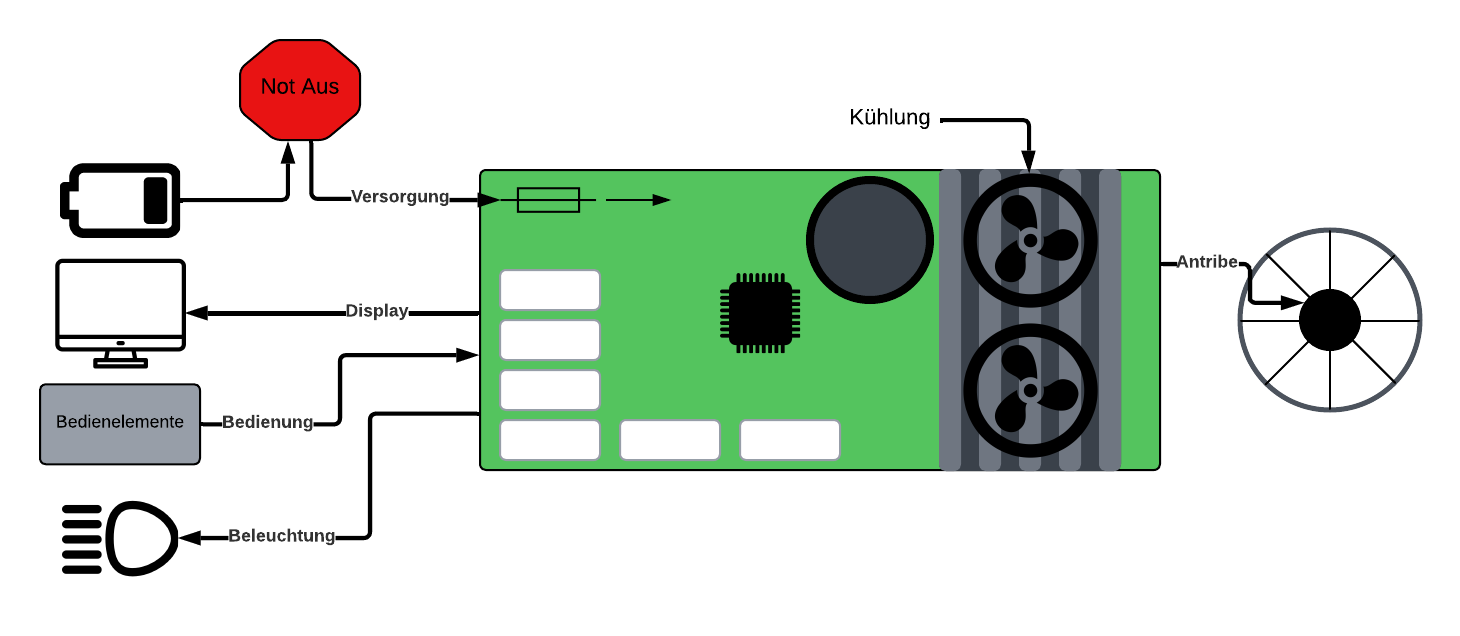
\includegraphics[width=14cm]{Bilder/Schaubild elektrik.PNG}
\caption{Vereinfachtes Steuergerät}
\label{ECU_sys}
\end{center}
\end{figure}

Das Steuergerät des E-Bikes bietet folgende Hauptfunktionen:
BLDC-Heckmotor-Antrieb: 3-Phasen H brücke für den Antriebe eines bürstenlosen Gleichstrommotor (Brushless DC/BLDC).
Beleuchtungselemente:
Integrierte LED-Vorder- und Rücklichter sorgen für Sichtbarkeit und Sicherheit.
Blinkerelemente und Bremslicht für Richtungsanzeigen.
Darstellung wichtiger Betriebsdaten über LCD:
Spannung, Strom, Temperatur,Geschwindigkeit,Fehler Code.
Integrierte Temperatur-Überwachung mit diskreter Lüfter Ansteuerung.

\section{Bedienung}

\begin{figure}[ht]
\begin{center}
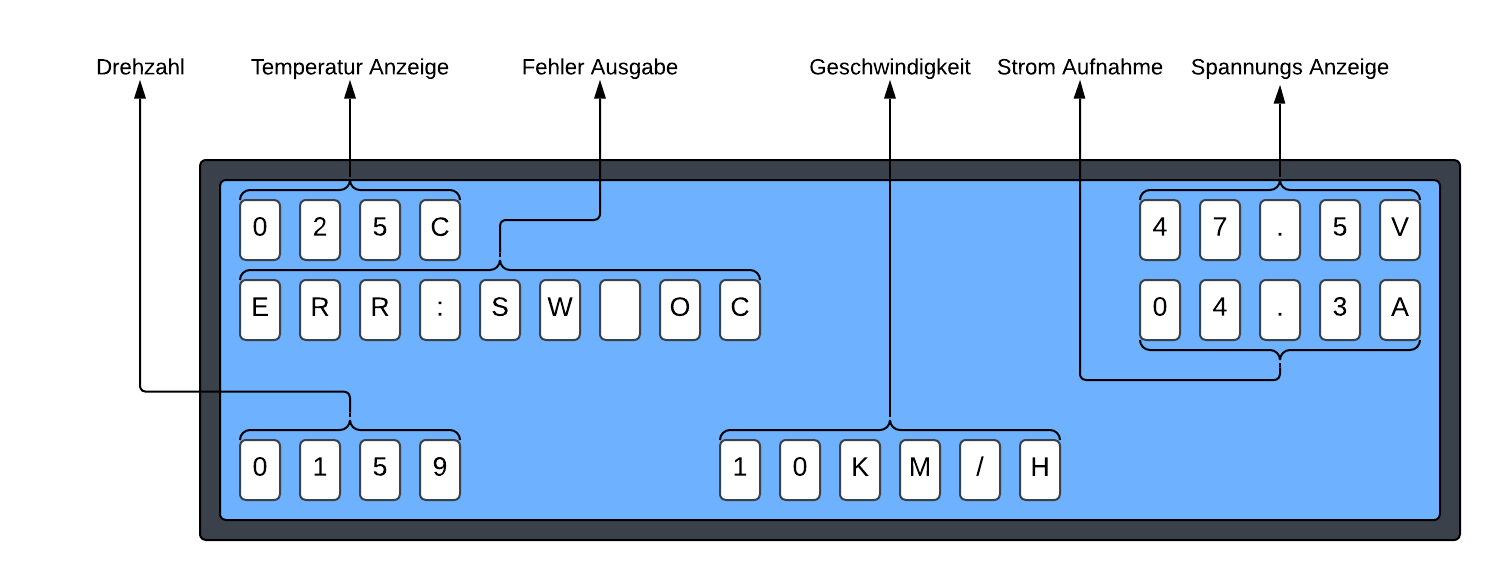
\includegraphics[width=14cm]{Bilder/Display.PNG}
\caption{Display Ausgabe}
\label{display}
\end{center}
\end{figure}

Die verschiedene Bedienelemte für den Benutzer befinden sich am Lenker in einem Motorrad ähnlichem system:
\textbf{E-Stop}: Deaktiviert das Selbsthalte-Relais und schaltet das Steuergerät aus.
\textbf{E-Start}: Aktiviert das Gerät und betätigt das Selbsthaltesystem, wodurch das E-Bike in den Betriebsmodus versetzt wird.
\textbf{Bremshebel}:
Aktiviert die Bremslichter.
Schaltet die Motorbremse am Hinterrad ein, um eine zusätzliche Verzögerung zu bieten.
\textbf{Gasgriff}: Reguliert die Motorleistung und steuert die Geschwindigkeit.
\textbf{Beleuchtung}:
\textbf{Taster Ablendlicht}: Schaltet das Ablendlicht und den Rückstrahler ein.
\textbf{Taster Blinker Links/Blinker Rechts}: Steuert die Blinkerelemente für die jeweilige Fahrtrichtung.
Diese Funktionen und Eingabemöglichkeiten stellen sicher, dass das E-Bike sowohl sicher als auch benutzerfreundlich im Betrieb ist.\\

\newpage
\section{Sicherheitsfunktionen}

\begin{figure}[ht]
\begin{center}
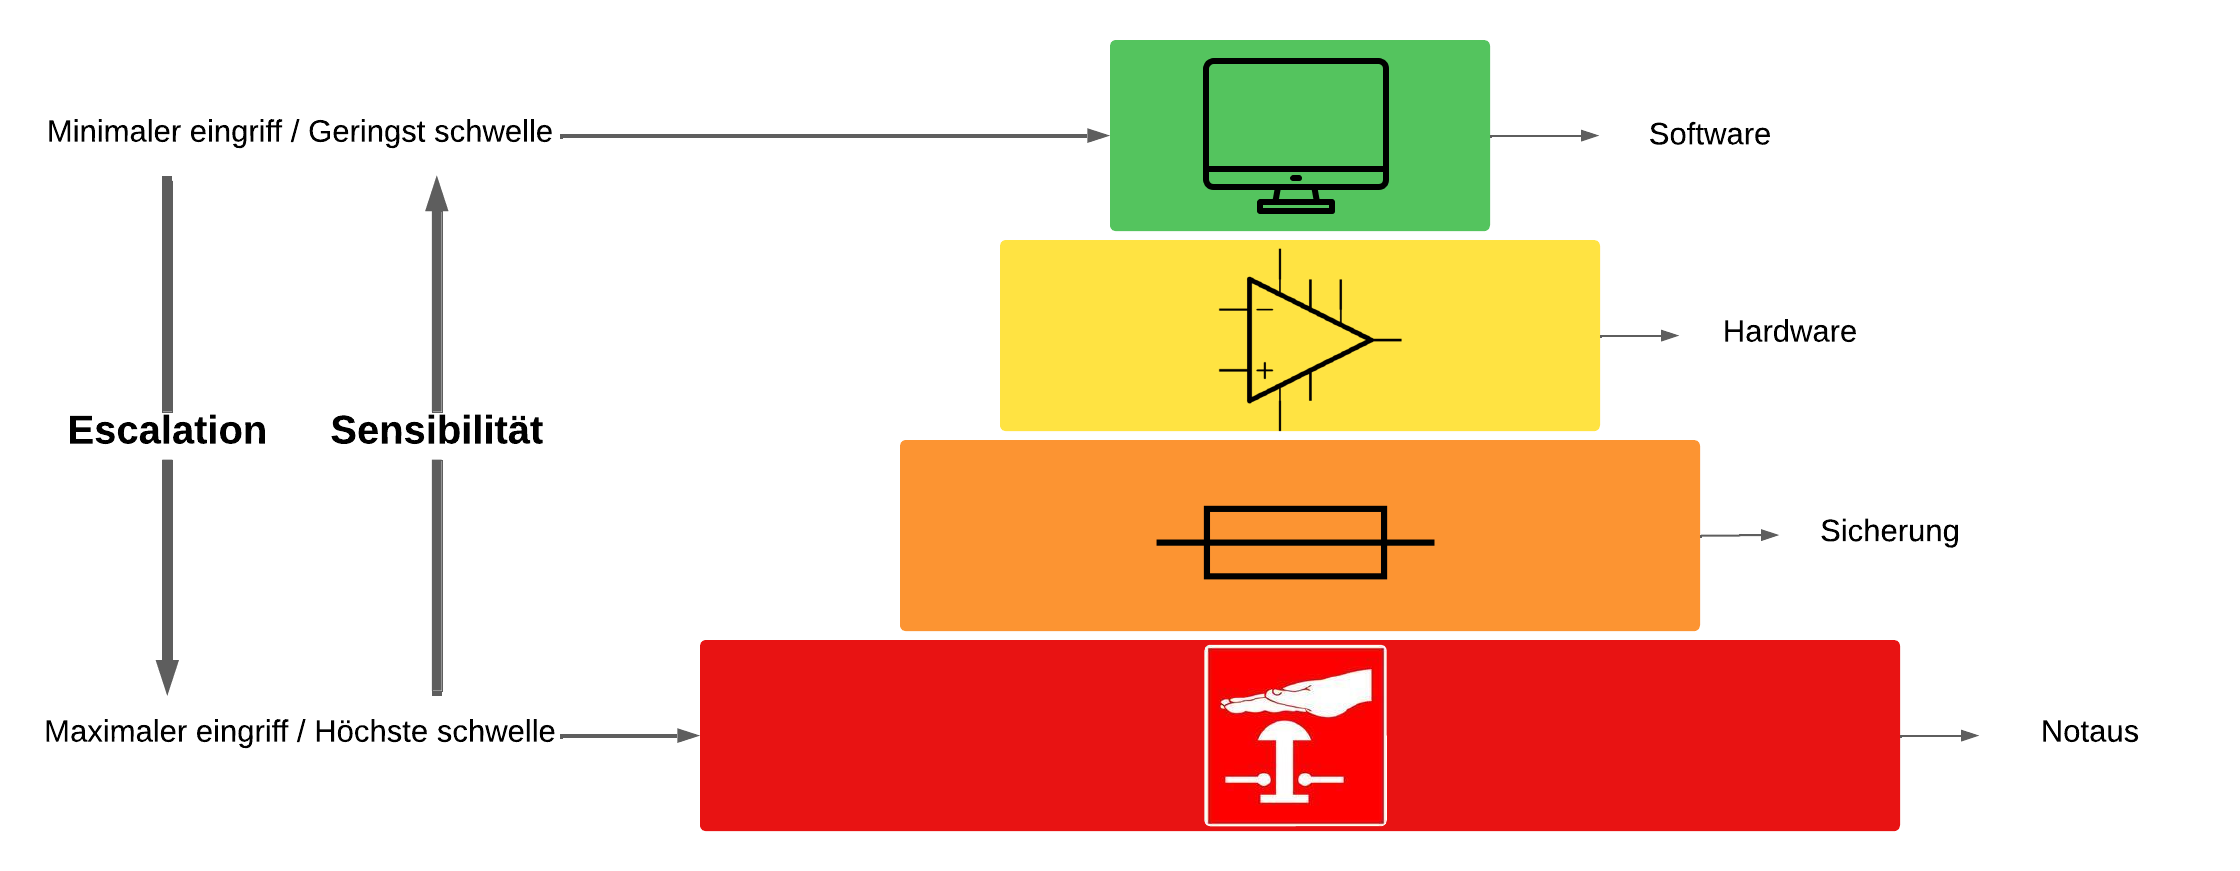
\includegraphics[width=13cm]{Bilder/Safety.PNG}
\caption{Sicherheitsfunktion}
\label{safety}
\end{center}
\end{figure}

\textbf{1 Software}\\
Auslösung: Messvorrichtungen überwachen Spannung, Strom und Temperatur. Überschreiten diese Werte festgelegte Schwellen, wird der Lastbetrieb automatisch abgeschaltet.
Eingriff: Das Gerät wechselt in einen Sicherheitszustand, aus dem es sich selbstständig zurücksetzen kann, sobald die Bedingungen wieder im Normalbereich liegen.\\
\textbf{2 Hardware}\\
Auslösung: Hardwarebasierte Messvorrichtungen erkennen Spannungen, Ströme oder Temperaturen außerhalb der spezifizierten Werte und schalten das Gerät ab.
Eingriff: Das Gerät wechselt in einen Sicherheitszustand, der nur durch einen manuellen Neustart wieder verlassen werden kann.\\
\textbf{3 Sicherung}\\
Auslösung: Stromkreise für 48V (25A) und 12V (3A) sind durch Sicherungen gegen Kurzschlüsse geschützt.
Eingriff: Bei Überlast oder Kurzschluss wird das Gerät außer Betrieb gesetzt. Zum Wiederinbetriebnehmen müssen die betroffenen Stecksicherungen ersetzt werden.\\
\textbf{4 Notaus}\\
Auslösung: Im Notfall betätigt der Nutzer den Notaus-Schalter.
Eingriff: Das Gerät wird sofort vom Akku getrennt und vollständig stromlos gemacht, um maximale Sicherheit zu gewährleisten.\\
\textbf{Hinweis zu BMS-Schutzfunktionen}\\
Das im Akku integrierte Battery Management System (BMS) verfügt zusätzlich über Schutzvorrichtungen gegen Überstrom, Unterspannung und Überhitzung. Diese Funktionen sind unabhängig von den hier beschriebenen Sicherheitsmaßnahmen und waren nicht Teil der Projektarbeit. Dennoch tragen sie wesentlich zur Gesamtsicherheit des Systems bei.

\part{Schaltplan, Layout und Software}
\chapter{Schaltplan}
In diesem Abschnitt der Dokumentation werden die einzelnen Teile des Schaltplans vorgestellt und detailliert beschrieben. Der vollständige, ununterbrochene Schaltplan ist Im Anhang oder Digital auf GitHub unter: github.com/leonreeh/E-Bike-ECU $\rightarrow$ RESC\_V2 Hardware $\rightarrow$ RESC\_V2 Schematic.pdf\\
Zur besseren Übersicht und Verständlichkeit des Schaltplans wird die folgende Namensgebung für Signale verwendet:\\
\textbf{SENSE} – Signal eines analogen Ausgangs (z. B. Spannungsmessung).\\
\textbf{DI} – Digitaler Eingang (Digital-Logik-Eingang des Mikrocontrollers).\\
\textbf{DO} – Digitaler Ausgang (Digital-Logik-Ausgang des Mikrocontrollers).\\
\textbf{¯¯¯} – Invertierung (Signal arbeitet als Active Low – ausgelöst bei Pegel 0).

\subsection{Kernbauteile}

\begin{tabular}[h]{l|c|r}
\textbf{Bauteil} & \textbf{Name} & \textbf{Beschreibung} \\
\hline
Mikrocontroller & STM32F405RGT6 & 32bit ARM 1024 FLASH 192kB SRAM \\
\hline
Abwärtswandler & LMR36520 & 2,5A DC/DC Converter 4-65V\\
\hline
Brücken Treiber & IR2101S & Bootstrap Brückentreiber\\
\hline
Power Mosfet & IPB035N08N3GATMA & 80V/100A NMos\\  
\hline
Leistungs Relais & JD2912-1Z-12VDC & 12V/40A DC\\
 \hline
Akkustecker & XT90 & 500V/40A DC\\
\hline
Motorstecker & MT60 & 500V/30A DC\\
\hline
Systemstecker & JST-XH Serie & 250V/3A DC\\
\hline
\end{tabular}

\section{Netzteil}
Das Netzteil bildet das Herzstück der Energieversorgung und stellt sicher, dass alle elektronischen Komponenten des Systems mit den benötigten Spannungen und Strömen versorgt werden. Es gewährleistet einen stabilen Betrieb der Elektronik.
\textbf{Funktionalität:}\\
Selbsthalterelais für zuverlässiges Einschalten, für zusätzlichen Schutz gegen Vibrationen und erschüttern wurde hier ein KFZ Relais gewählt das eine besseres Haltemoment als herkömmliche printrelais bietet. \\
48V Hochleistungsversorgung für den Motor\\
DC/DC-Wandler (12V) für Beleuchtung und leistungs Elemente (max. 2.5A)\\
DC/DC-Wandler (5V) für Display und logik Elemente (max. 2A)\\
LDO-Regler (3.3V) für eine besonders stabile Versorgung auf Logik-Ebene.\\
\textbf{Besonderheiten:}
Messung des Eingangsstroms
Messung der Eingangsspannung
Hardwarebasierte Überstromerkennung
Hardwarebasierte Unterspannungserkennung.
\newpage

\subsection{Powertrain}

\begin{figure}[ht]
\begin{center}
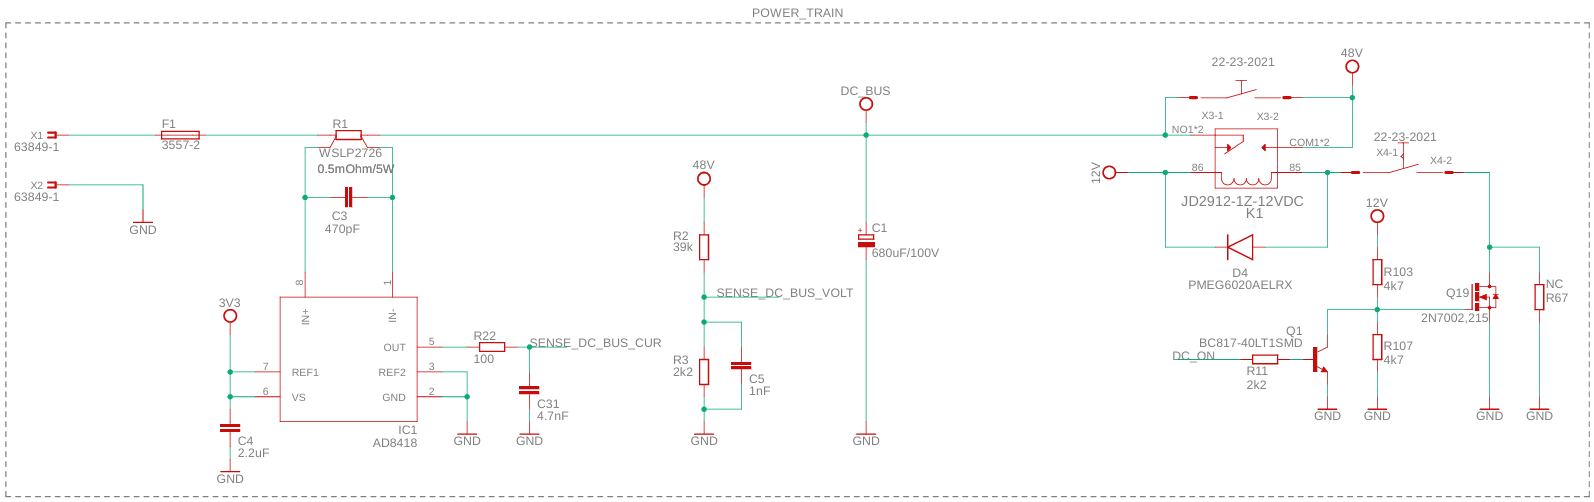
\includegraphics[width=14cm]{Bilder/Powertrain.PNG}
\caption{RESC\_V2 Schaltplan Seite 2}
\label{Powertrain}
\end{center}
\end{figure}

In der ersten Funktionsgruppe, dem „Power Train“, sind alle Komponenten zusammengefasst, die in direkter Verbindung mit dem Akku stehen und den Hochleistungspfad für den Motortreiber bilden.
KFZ-Stecksicherung F1: Schützt den Akku vor Überstrom und Kurzschlüssen.
Shunt R1: Misst den Eingangsstrom und ermöglicht eine präzise Erfassung des Stromverbrauchs.
Spannungsteiler R2/R3: Dient zur Messung der Eingangsspannung und leitet die Daten an die Steuerung weiter.
Bulk-Kondensator C1: Glättet Spannungsspitzen und stabilisiert die Eingangsspannung, um Schwankungen auszugleichen.
Selbsthalte-KFZ-Relais K1: Schaltet die versorgungsspannung des Niederleistungspfad und sorgt dafür, dass das System sicher ein und ausgeschaltet werden kann.
Diese Funktionsgruppe ist essenziell für die sichere Versorgung des Motortreibers und bildet die Grundlage für die gesamte Energieversorgung des E-Bikes.

\subsection{DC/DC}

Um unnötige Verlustleistung zu vermeiden und die Komplexität des Netzteils gering zu halten, werden für die Versorgung der Elektronik lediglich drei Spannungsebenen benötigt:\\
\textbf{12V} – System-Leistungsspannung als Versorgung der Beleuchtung, Lüfter, Relais und des Motortreibers.\\
\textbf{5V} – Sensor- und Displayversorgung für Motor-Hall-Sensoren und des LCD-Displays.\\
\textbf{3.3V} – System-Logikspannung für die Versorgung des Mikrocontrollers, Operationsverstärkers und der analogen Signale.\\
Durch die Reduzierung auf diese drei Spannungspegel wird der Aufbau des Netzteils vereinfacht, während gleichzeitig eine stabile und effiziente Energieversorgung für die verschiedenen Baugruppen gewährleistet wird.\\
\newpage

\begin{figure}[ht]
\begin{center}
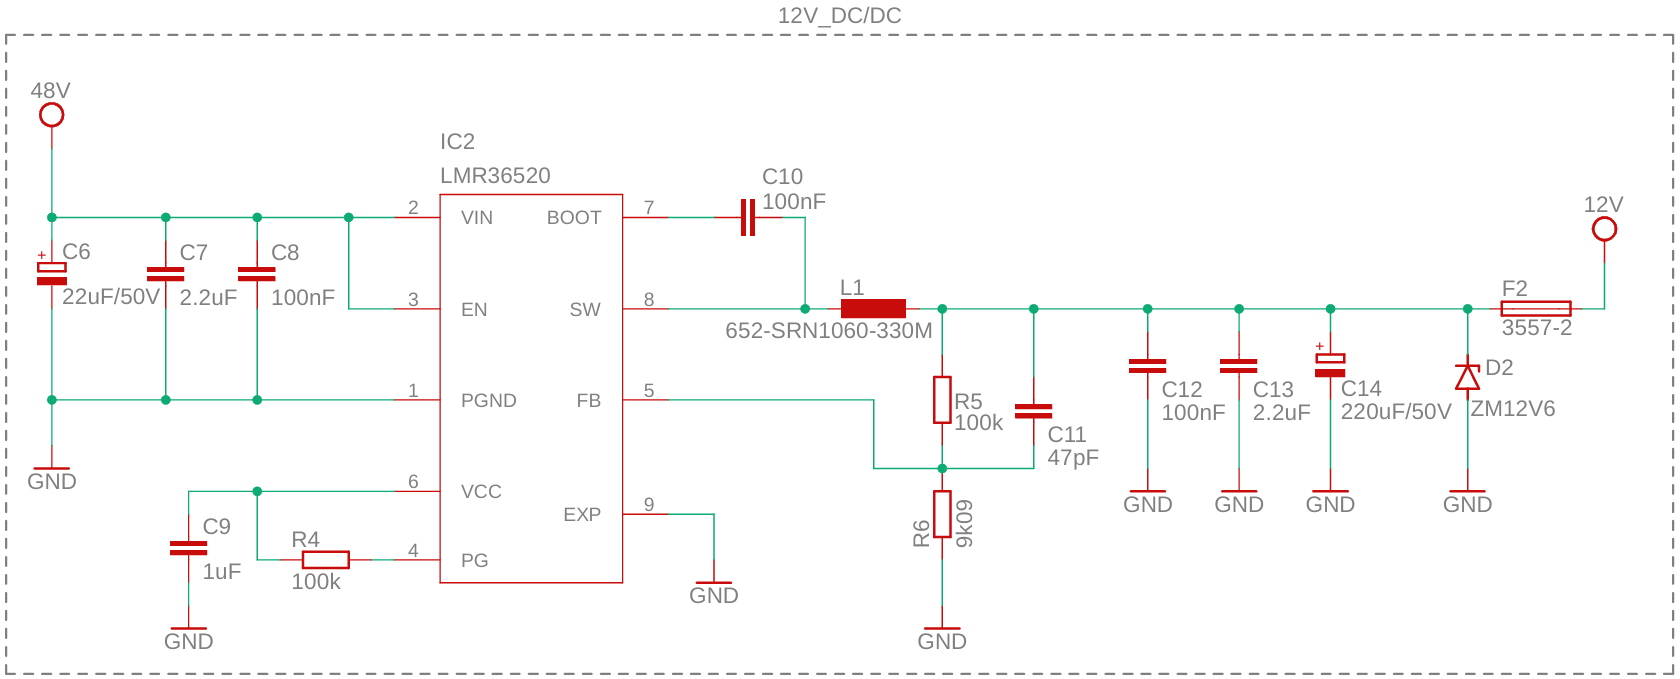
\includegraphics[width=12cm]{Bilder/DCDC.PNG}
\caption{12V Abwärtswandler RESC\_V2 Schaltplan Seite 2}
\label{DCDC}
\end{center}
\end{figure}

Die Beschaltung des LMR36520 entspricht dem TI-Referenzdesign (Datenblatt Abschnitt 9.2 Typical Application) und wurde um eine 12V6 Suppressordiode (Z-Diode) ergänzt, um das System vor Überspannung zu schützen. Diese zusätzliche Schutzmaßnahme trägt zur Erhöhung der Zuverlässigkeit und Langlebigkeit der Spannungsversorgung bei, indem sie Spannungsspitzen effektiv absorbiert und so empfindliche Schaltungsteile schützt
Die Induktivität L1 wurde gemäß den Richtlinien im Datenblatt des LMR36520 dimensioniert (Datenblatt Abschnitt 9.2.1.2.3 – Inductor Selection).

\subsection{Protection circuits}

\begin{figure}[ht]
\begin{center}
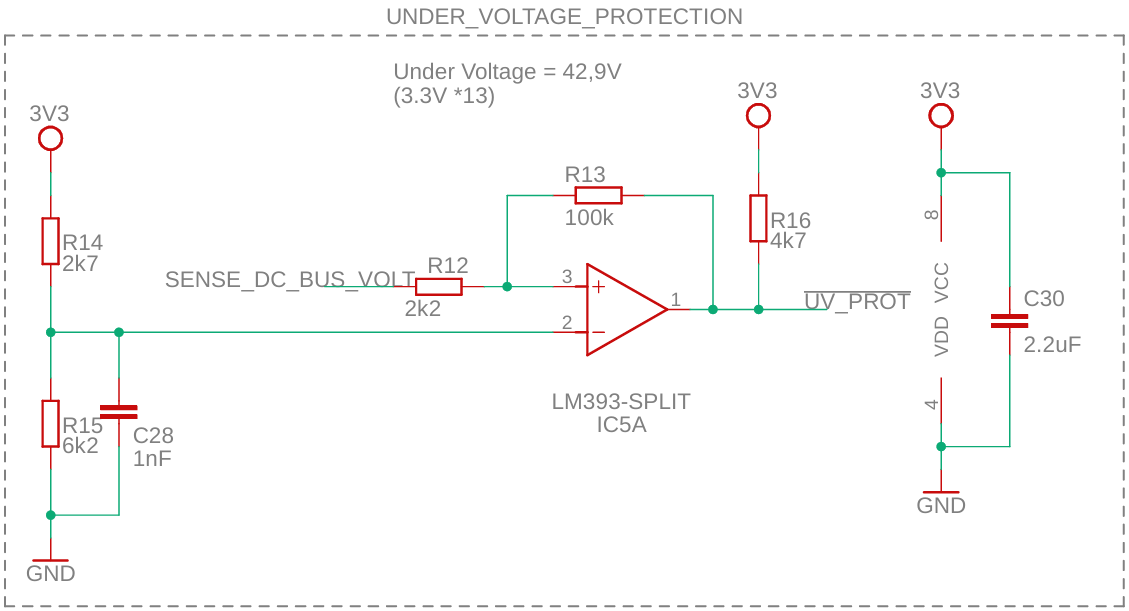
\includegraphics[width=12cm]{Bilder/Protection circuit.PNG}
\caption{Unterspannungsschutz RESC\_V2 Schaltplan Seite 2}
\label{UV}
\end{center}
\end{figure}

Für die Umsetzung der Sicherheitsfunktion auf Hardware-Ebene wurde eine einfache Komparatorschaltung implementiert, die die drei Messgrößen (Spannung, Strom, Temperatur) überwacht. Beim Überschreiten vordefinierter Schwellenwerte sendet sie ein „Fehler“-Signal an den Mikrocontroller.
Im Beispiel in Abbildung \ref{UV} wurde zum Schutz vor Tiefentladung des Akkus eine Spannung von 42,9 V festgelegt. Bei 13 in Reihe geschalteten Zellen ergibt sich daraus eine minimale Zellenspannung von 3,3 V.
Über-Strom und -Temperatur Erkennung werden mit der gleichen Schaltung implementiert und nach relevanten Kriterien dimensioniert.

\subsection{Hardware Interrupt}

\begin{figure}[ht]
\begin{center}
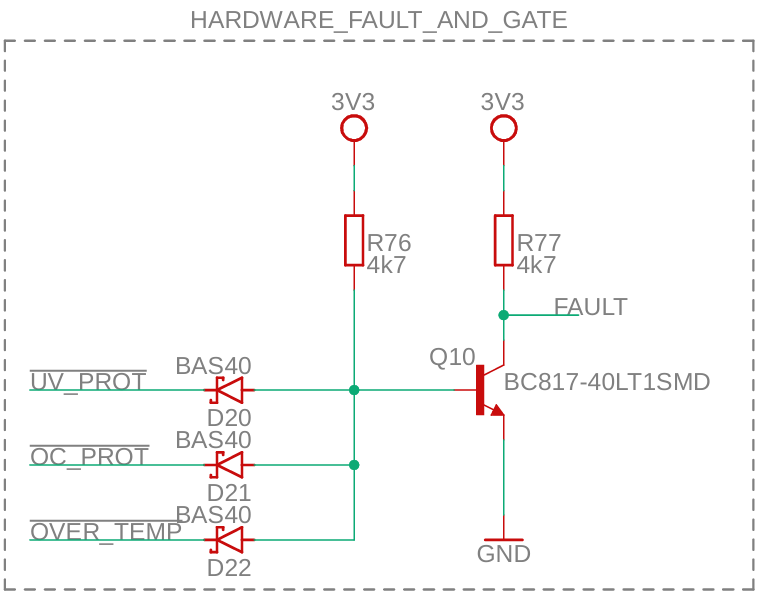
\includegraphics[width=12cm]{Bilder/FaultAnd.PNG}
\caption{Oder Gatter RESC\_V2 Schaltplan Seite 3}
\label{orGate}
\end{center}
\end{figure}

Um sicherzustellen, dass die Elektronik im Falle eines Hardware-Fehlers immer konsistent reagiert, werden die drei Hardware-Fehlersignale (Strom, Spannung, Temperatur) über ein ODER-Gatter zusammengefasst.
Das resultierende \textbf{"FAULT"}-Signal wird auf einen Interrupt-Pin des Mikrocontrollers gelegt, sodass dieser bei einem Fehler schnellstmöglich reagieren kann. Durch diese einfache Hardwareschaltung können zwei zusätzliche Interrupt-Pins eingespart werden, da alle drei Fehlersignale zum selben Sicherheitszustand führen sollen und daher keinen eigenen Interrupt-Pin benötigen.

\subsection{Mikrocontroller}
Der STM32F405RGT6 bildet das zentrale Steuerungselement des Systems und koordiniert die gesamte Elektronik. Er übernimmt die Verarbeitung und Weiterleitung von Signalen, die Überwachung der Systemparameter, die Kommunikation mit anderen Modulen und nicht zuletzt die Ansteuerung der Motor H-Brücke.

\begin{figure}[ht]
\begin{center}
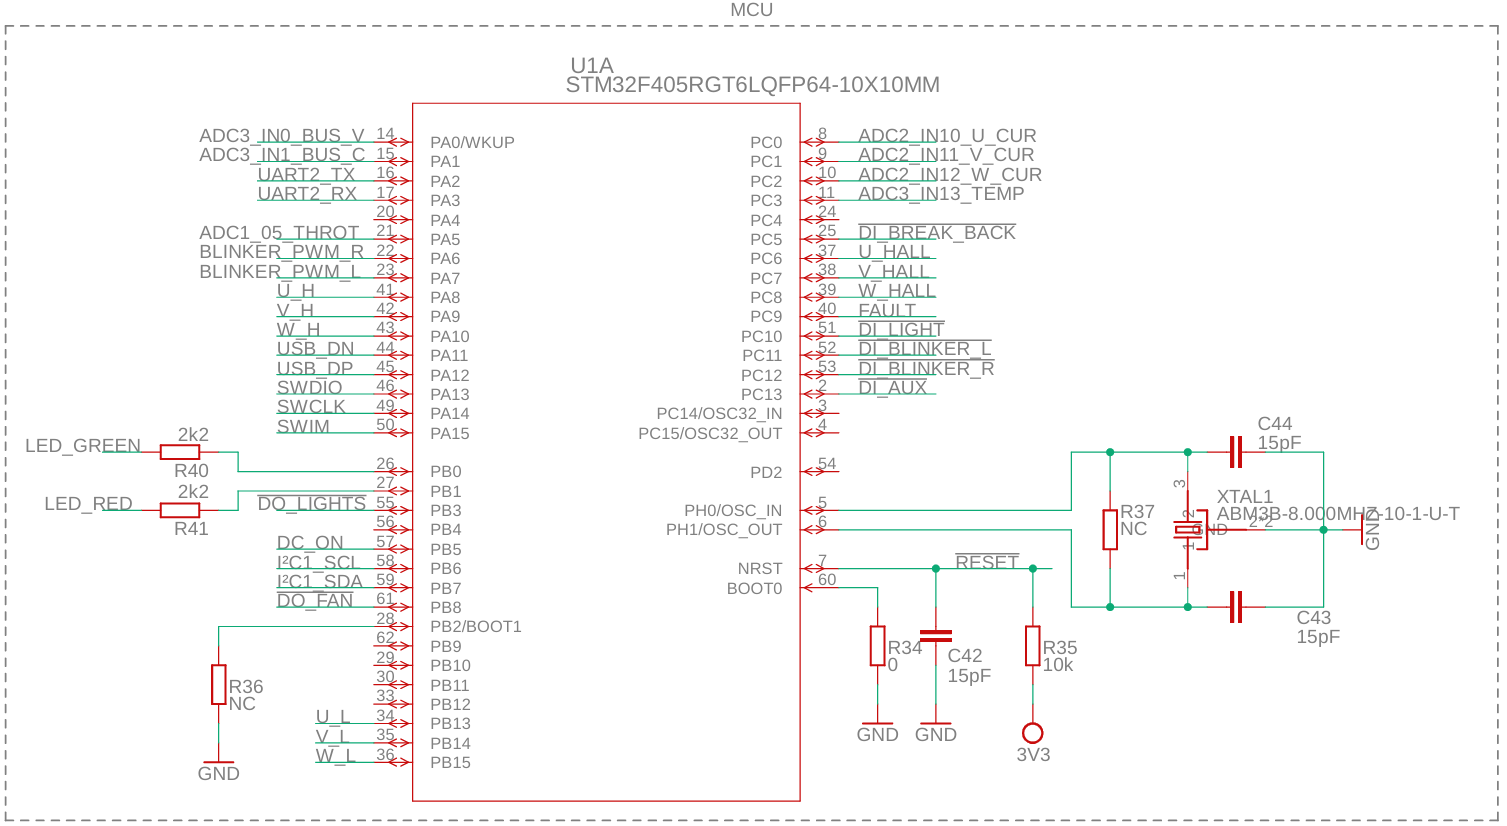
\includegraphics[width=10cm]{Bilder/Pinning.PNG}
\caption{Mikrocontroller Pinbelegung RESC\_V2 Schaltplan Seite 3}
\label{mcu}
\end{center}
\end{figure}

Die Pin-Belegung des Mikrocontrollers wurde mit hilfe des STM32CubeIDE-Konfigurators festgelegt. Dabei wurden die Timer-PWM-Kanäle, Interrupt-Pins und ADCs konfiguriert.
Als Referenz diente der \textbf{VESC 6.4 Schaltplan}, der maßgeblich zur Auswahl des Mikrocontrollers beitrug. Diese Vorgehensweise ermöglichte die Funktions-kritisch Aspekte der notwendigen Peripheriefunktionen für die Motorsteuerung und Systemüberwachung zu implementieren.

\begin{figure}[ht]
\begin{center}
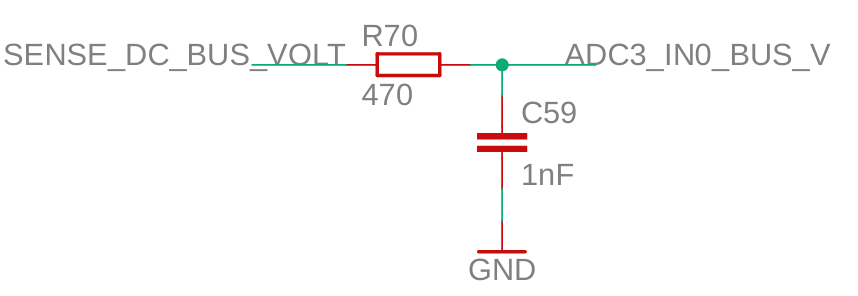
\includegraphics[width=6cm]{Bilder/ADC.PNG}
\caption{RC-Filter RESC\_V2 Schaltplan Seite 3}
\label{ADC}
\end{center}
\end{figure}

Zur Entstörung der Analogsignale sind alle ADC-Pins des Mikrocontrollers mit einem RC-Glied ausgestattet.
Das RC-Glied dient dazu, hochfrequente Störungen zu filtern und sicherzustellen, dass die an den ADC-Eingängen gemessenen Werte stabil und präzise sind. Dies trägt zur Verbesserung der Signalqualität und zur Reduzierung von Messfehlern bei.
\newpage

\begin{figure}[ht]
\begin{center}
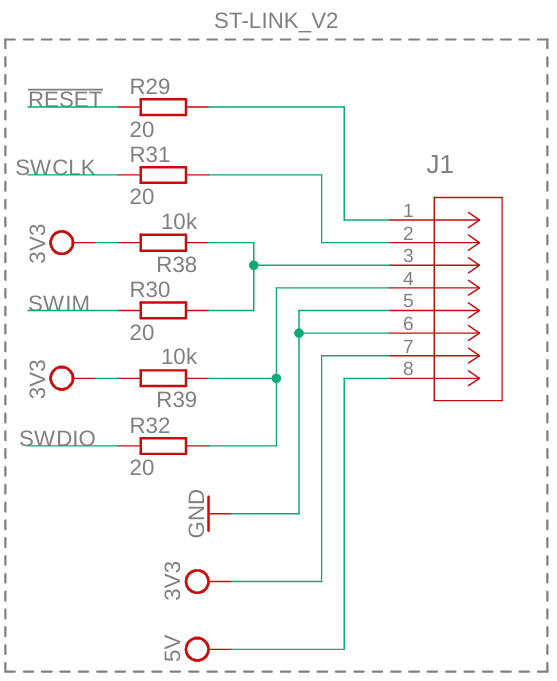
\includegraphics[width=6cm]{Bilder/ST-Link.PNG}
\caption{ST-Link RESC\_V2 Schaltplan Seite 3}
\label{ST_LINK}
\end{center}
\end{figure}

Standard SWD-Schnittstelle zum Programmieren und Debugging von STM-Mikrocontrollern. Die Schnittstelle ist vollständig kompatibel mit dem ST-Link V2 über das Serial Wire Debug (SWD)-Protokoll.


\begin{figure}[ht]
\begin{center}
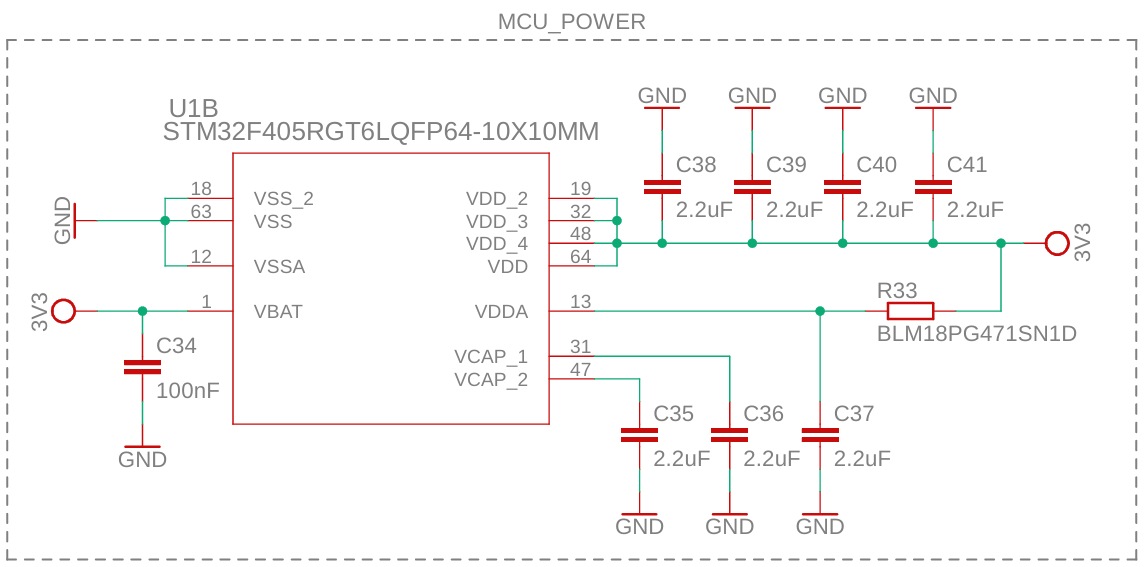
\includegraphics[width=8cm]{Bilder/MCU-Power.PNG}
\caption{Mikrocontroller Versorgung RESC\_V2 Schaltplan Seite 3}
\label{mcu_psu}
\end{center}
\end{figure}

Jeder Versorgungspin des Mikrocontrollers ist mit einem eigenen 2,2 µF Kondensator ausgestattet, um eine möglichst stabile Spannungsversorgung zu gewährleisten. Der ADC-Referenzpin (VDDA) ist zusätzlich mit einem Ferritfilter gegen Störungen geschützt.
\newpage
\subsection{BLDC}
Für die Implementierung des BDLCs wird eine drei Phasen H-Brücke benötigt. dies wurde durch den \textbf{Infineon 2101S} Bootstrap-H-Brücken-Treiber und leistungsstarke \textbf{IPB035N08N3GATMA}-Power-MOSFETs realisiert.

\begin{figure}[ht]
\begin{center}
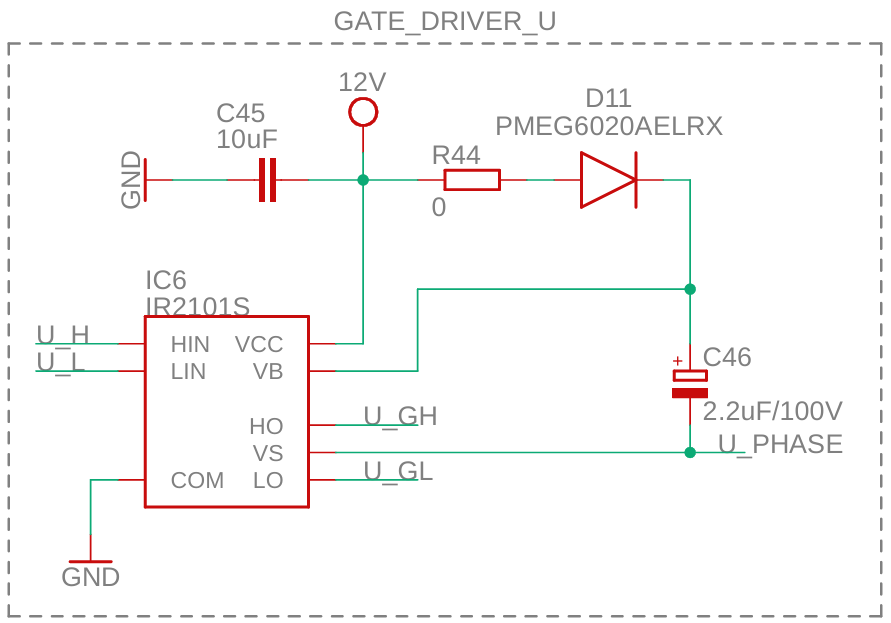
\includegraphics[width=12cm]{Bilder/BLDCDriver.PNG}
\caption{H-Brücken Treibe RESC\_V2 Schaltplan Seite 4}
\label{GateDriver}
\end{center}
\end{figure}

Das Infineon 2101S Treiber IC wurde gewählt für seine einfache Implementierung, Ansteuerung, integrierte Bootstrap-Schaltung und Short Protection. Die Referenzschaltung wurde um einen Vorwiderstand R44 erweitert der es ermöglicht den Ladestrom von C46 zu dimensionieren. \\
Dimensionierung des Bootstrap-Kondensators C46 gemäß der Faustregel:\\ $C_{bootstrap}\geq10\times C_{gs}$ ($C_{gs}$ = 2.2nF Gate-Kapazität der MOSFETs)
Diese Dimensionierung stellt sicher, dass der Treiber auch bei hohen Schaltfrequenzen zuverlässig arbeitet und eine stabile Gate-Spannung bereitgestellt wird.
\newpage

\begin{figure}[ht]
\begin{center}
\includegraphics[width=10cm]{Bilder/HBrücke.PNG}
\caption{H-Brück RESC\_V2 Schaltplan Seite 4}
\label{HBridge}
\end{center}
\end{figure}

Die Strom- und Drehmomentregelung erfolgt durch eine Shunt-Messung direkt am Phasenabgriff der H-Brücke, wodurch der tatsächliche Phasenstrom präzise erfasst und eine genauere Motorregelung ermöglicht wird. Zur Entlastung der MOSFET-internen Body-Dioden und zur Reduzierung der thermischen Belastung, insbesondere bei schnellen Schaltvorgängen und hohen Strömen, werden externe Freilaufdioden (D16/D17) parallel zu den MOSFETs geschaltet. Jedes MOSFET ist mit einem Pull-Down-Widerstand am Gate versehen, um ungewolltes Einschalten durch Leckströme zu verhindern und einen sicheren Sperrzustand zu gewährleisten. Zusätzlich ist jede H-Brücke mit einem 2,2 µF Kondensator ausgestattet, der Schalt- und Spannungsspitzen reduziert, die MOSFETs vor Überspannungen schützt und zur Glättung der Phasenspannung beiträgt.
\newpage
\subsection{Beleuchtung}
Die Beleuchtungseinheit steuert die LED-Beleuchtungselemente mittels diskreter MOSFET-Treibern. Ihr primärer Zweck ist die Gewährleistung der gesetzlich vorgeschriebenen sowie funktionalen Fahrzeugbeleuchtung für den Straßenverkehr, wodurch Sicherheit und Sichtbarkeit erhöht werden. Die Beleuchtung umfasst Abblendlicht, Rücklicht, Bremslicht und Blinker, wobei letztere durch Software-PWM geregelt werden, um eine flexible Lichtsteuerung zu ermöglichen.

\begin{figure}[ht]
\begin{center}
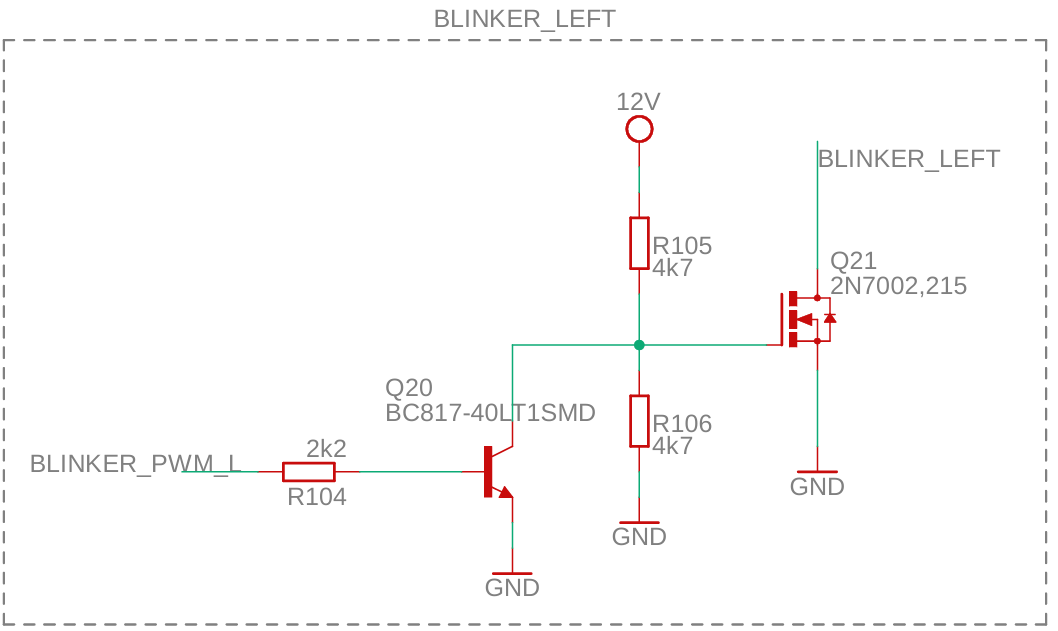
\includegraphics[width=12cm]{Bilder/Blinker.PNG}
\caption{H-Brücken Treibe RESC\_V2 Schaltplan Seite 5}
\label{blinker}
\end{center}
\end{figure}

Alle Beleuchtungs-LEDs verwenden die gleiche Treiberbeschaltung. Der einzige Unterschied zwischen den Treibern liegt in der Größe der MOSFETs, die entsprechend der Leistungsaufnahme der jeweiligen LED-Gruppen dimensioniert werden.
\newpage
\subsection{Temperatur}
Die Temperaturüberwachung dient dem Schutz der Leistungskomponenten durch eine Messung und  Steuerung der Kühlung. Ein NTC-Sensor am Kühlkörper erfasst die Temperatur, während eine MOSFET-basierte Lüftersteuerung, mit optionalem PWM-Betrieb, eine bedarfsgerechte Kühlung ermöglicht. Eine OP-basierte Hardware-Schaltung erkennt Übertemperaturen und reagiert entsprechend, um Schäden an den Leistungskomponenten zu verhindern.
\\

\begin{figure}[ht]
\begin{center}
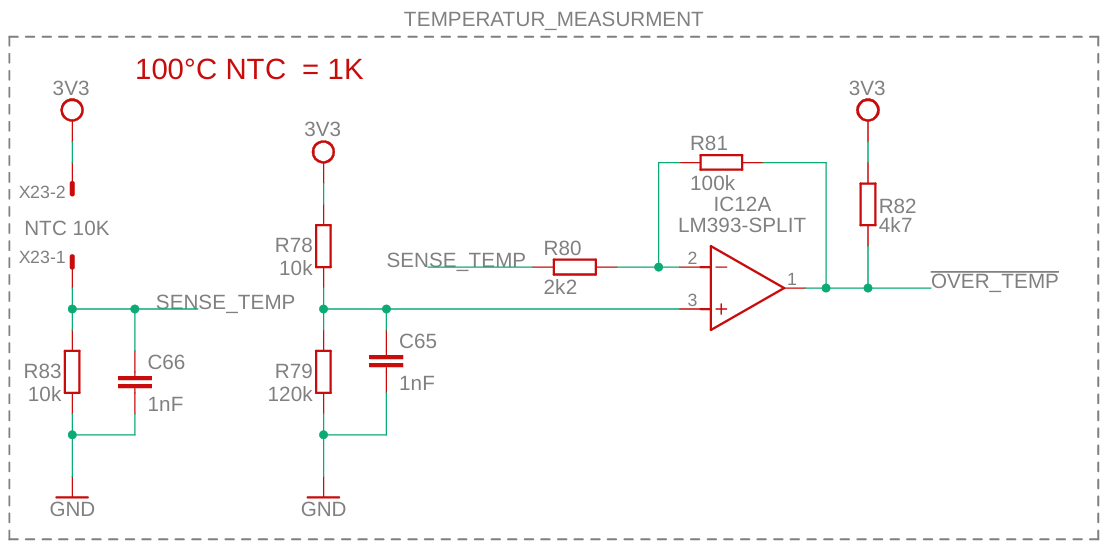
\includegraphics[width=14cm]{Bilder/Temp.PNG}
\caption{Temperaturmessung RESC\_V2 Schaltplan Seite 6}
\label{temp}
\end{center}
\end{figure}

Der \textbf{NTC-Widerstand (R84)} ist direkt am Kühlkörper befestigt, um eine kontinuierliche Überwachung der Systemtemperatur zu gewährleisten. Die Lüftersteuerung erfolgt softwareseitig über eine \textbf{Hysterese}, wobei der Lüfter eingeschaltet wird, sobald die Temperatur \textbf{80°C} übersteigt, und wieder abgeschaltet wird, sobald sie unter \textbf{60°C} fällt. Falls die softwaregesteuerte Regelung nicht ausreicht, um den Temperaturanstieg zu begrenzen, greift eine hardwarebasierte Fehlererkennung bei \textbf{120°C} ein. Diese löst automatisch Schutzmaßnahmen aus, um die MOSFETs vor Überhitzung und möglichen Schäden zu bewahren.\\
Für das Ansteuern von zwei 40mm PC-Lüftern wird ein MOSFET-Treiber verwendet. Die Steuerung der Lüfter erfolgt über den Digital Output DO-FAN, der wahlweise im PWM-Betrieb oder im Digitalbetrieb arbeiten kann.
\newpage
\subsection{IO}
Das Eingabe- und Ausgabe-Modul ermöglicht die Interaktion zwischen Benutzer und System durch die Erfassung von Eingabeelemente wie Taster sowie die Ausgabe von Systeminformationen auf einem Kommunikationsschnittstelle. Die Kommunikationsschnittstelle kann wahlweise über eine I²C- oder UART Daten übertragen, wodurch eine flexible Integration in verschiedene Systemarchitekturen ermöglicht wird wie z.b LDC-Displays oder mehr Fortgeschrittene TFT Touch Tabletts.

\begin{figure}[ht]
\begin{center}
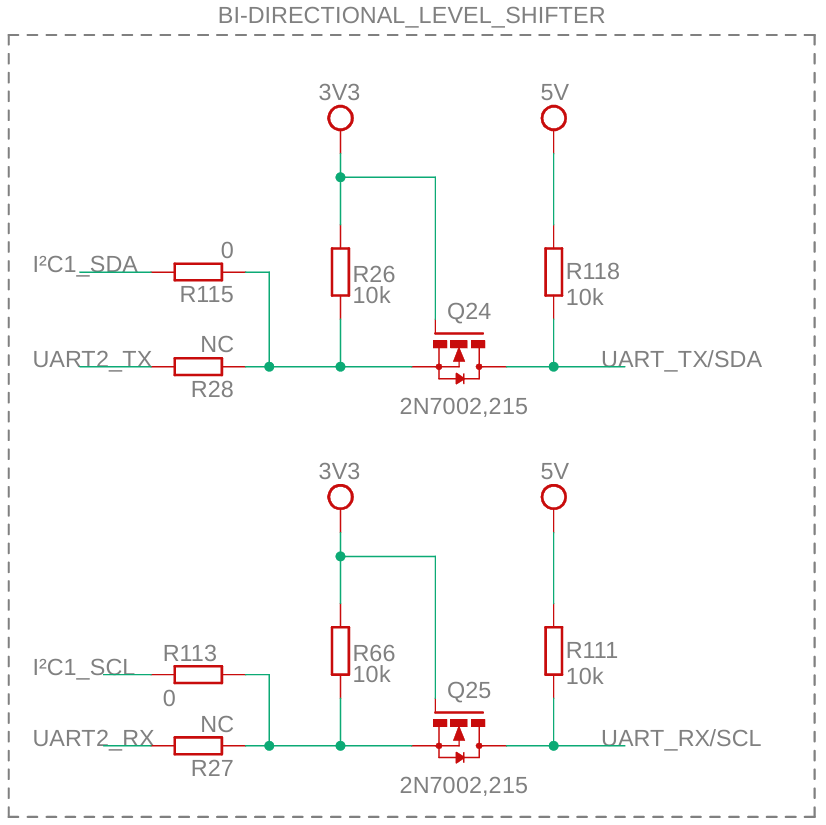
\includegraphics[width=10cm]{Bilder/shifter.PNG}
\caption{Bidirektionaler-Levelshifter RESC\_V2 Schaltplan Seite 7}
\label{shifter}
\end{center}
\end{figure}

Die Konfigurierung der Kommunikationsschnittstelle, erfolgt über das bestücken der entsprechenden Widerstände (R28, R27 oder R115, R113). Diese Anpassungsmöglichkeit ermöglicht die Anbindung einer Vielzahl kompatibler Displays und Peripheriegeräte. Zur Sicherstellung der Kompatibilität mit Arduino-Komponenten, die auf einem 5V-Logiklevel arbeiten, ist die Schnittstelle zusätzlich mit einem Bidirektionalem 3.3V/5V-Level-Shifter ausgestattet. Dieser gewährleistet eine zuverlässige Kommunikation zwischen den Komponenten, unabhängig vom verwendeten Logikpegel.

\chapter{Layout}
In diesem Kapitel wird das Layout der Leiterplatte (PCB) detailliert beschrieben. Ziel ist es, die wichtigsten Designentscheidungen, Regelwerke und Dimensionierungen zu dokumentieren, um die optimale Funktion und Zuverlässigkeit des Systems sicherzustellen. Das angefertigte Layout finden Sie im Anhang oder digital auf: 
github.com/leonreeh/E-Bike-ECU $\Rightarrow$ RESC\_V2 Hardware $\Rightarrow$ RESC\_V2 PCB.pdf

\begin{figure}[ht]
\begin{center}
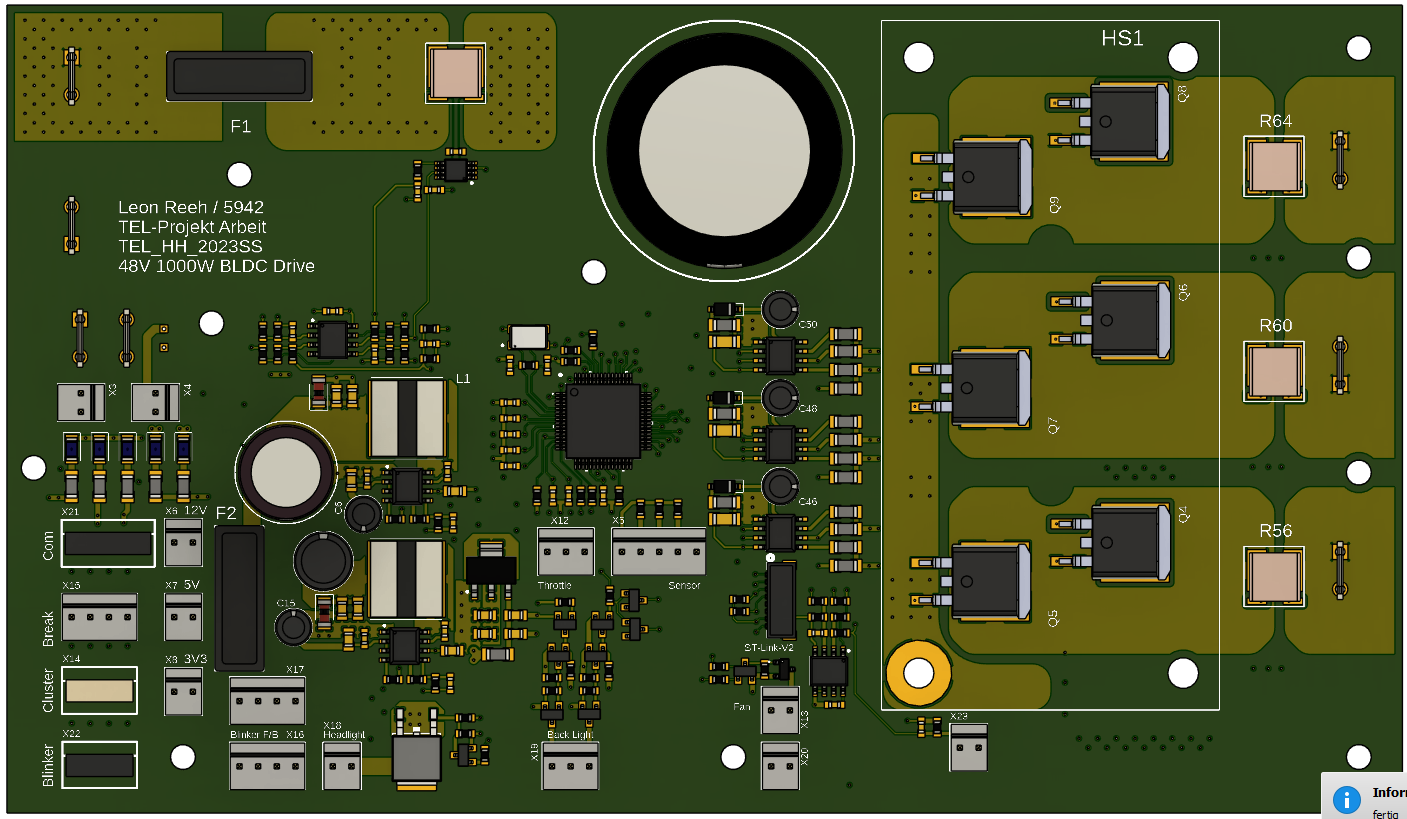
\includegraphics[width=14cm]{Bilder/PCB.PNG}
\caption{RESC\_V2 Leiterplatte}
\label{pcb}
\end{center}
\end{figure}
\newpage
\section{Design Regeln}
Für die Leiterplattenentwicklung wurden folgende Design-Regeln definiert:
\textbf{Leiterbahnbreiten und -abstände:} Signal-Leitungen werden mit einer Breite von 8 mil ausgeführt, während Versorgungsleitungen im Kleinspannungsbereich ($\geq$ 12 V) 20 mil breit sind. Für Hochleistungspfade beträgt die Mindestbreite 700 mil.
\textbf{Via-Dimensionierung:} Die Vias werden gemäß den Vorgaben des PCB-Herstellers (JLCPCB) dimensioniert und besitzen eine Bohrung von 0,3 mm.
\textbf{Isolationsabstände:} Im Signalbereich beträgt der Isolationsabstand 16 mil (entspricht dem Zweifachen der Signal-Leitungsbreite), im Versorgungsnetz 20 mil und im Hochleistungsbereich 100 mil.
\textbf{Bauteilplatzierung}: Die Bauteile werden entsprechend ihren Schaltplangruppen angeordnet, sodass jede Gruppe ein schlüssiges Layout bildet. Dabei gilt die Regel: Komponenten, die zusammenarbeiten, werden auch physisch zusammen platziert. Beispielsweise werden RC-Filter (Widerstand und Kondensator) direkt nebeneinander und so nah wie möglich am zu filternden Eingang positioniert.
\textbf{Lagenaufteilung:} Der Top Layer (Layer 1) dient als Hauptbestückungslayer, während der Bottom Layer (Layer 6) als Hilfslayer genutzt wird, insbesondere für die Platzierung von Abblock-Kondensatoren nahe an den Versorgungspins des Mikrocontrollers.

\section{PCB Dimensionierung}
Die Platine besitzt eine Abmessung von 190 × 110 mm. Die einzige kritische Vorgabe bezüglich der Außenmaße war, dass sie kleiner als 210 × 210 mm bleibt, damit das PCB-Trägergehäuse auf ein 3D-Druckbett passt.\\
Die Befestigung erfolgt über mehrere M3-Schrauben, die das PCB sicher im Gehäuse fixieren. Besondere Aufmerksamkeit wurde auf die Befestigung großer und schwerer Bauteile gelegt, ebenso wie auf Bereiche, die unter mechanischer Belastung stehen, beispielsweise Stecker und Kabel. Diese Maßnahmen minimieren Biegestress und Vibrationen der Elektronik.\\
Die Design-Toleranzen richten sich nach den Fertigungsvorgaben von JLCPCB:\\
PCB-Outline: ±0,2 mm\\
Pad-Pad-Abstand: 6 mil\\
Pad-Via-Abstand: 6 mil\\
Die Steckerplatzierung wurde so gestaltet, dass eine einfache Handhabung ermöglicht wird. Stecker sind daher möglichst nah am Platinenrand positioniert, wobei die Orientierung der Platine innerhalb des Gehäuses berücksichtigt wurde. Beispielsweise sind:

Stecker für den Motor auf der Rückseite, da sich der Motor hinter der Elektronik befindet.
Stecker für Bedienelemente auf der Vorderseite, da diese leicht zugänglich sein müssen.
Eine Ausnahme bilden der Stecker für den Motor-Hall-Sensor sowie der Stecker für den Analog-Gasgriff. Diese wurden in der Nähe des Mikrocontrollers platziert, um eine optimale Signalanbindung zu gewährleisten.

\section{Layer Design}
Um unerwünschte Störeinflüsse zu minimieren und die Signalqualität zu gewährleisten, wurden die sechs zur Verfügung stehenden Layer in spezifische Signalgruppen aufgeteilt. Dies ermöglicht eine klare Trennung von Leistungs- und Signalleitungen mit dem ziel elektromagnetische Störungen (EMI) zu reduzieren. Die Verteilung der Layer folgt einem logischen Aufbau, der sich an bewährten Industriepraktiken orientiert:\\

\begin{figure}[ht]
\begin{center}
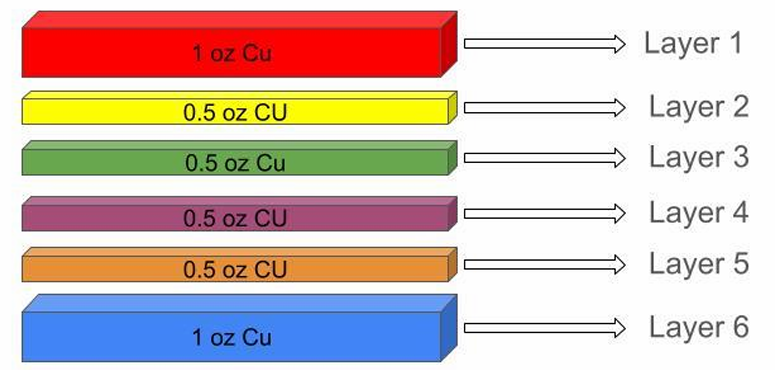
\includegraphics[width=8cm]{Bilder/LayerStack.PNG}
\caption{6-Layer PCB Stackup RESC\_V2 Layout}
\label{lstack}
\end{center}
\end{figure}

Layer:\\
1. Baugruppen- und Power-Layer\\
2. Signal-Ground-Layer\\
3. Primär Digital-Signal-Layer\\
4. Analog-Signal-Layer\\
5. Kleinspannungs-Power-Layer (12V, 5V, 3.3V)\\
6. Primär Power-Layer\\
\textbf{Layer 1 (Top-Layer – Hochstrom und Leistungsführung):} Layer 1\&6 tragen die Hauptlast der Leistungsversorgung. Da diese Layer die dickste Kupferschicht aufweist (1 oz Kupfer pro Layer), werden sie für die Führung der 48V Versorgung und der Motorphasenströme genutzt. Leiterbahnen, die große Ströme führen, wie z. B. die H-Brücken für den BLDC-Motor, werden auf diesem Layer platziert. Breite Leiterbahnen und großzügige Kupferflächen gewährleisten einen niedrigen Widerstand und vermeiden unerwünschte Erwärmung. Der Platzbedarf für Hochstromverbindungen wird optimiert, um Spannungsabfälle und Leistungsverluste zu minimieren.\\
\textbf{Layer 2 (Signal Ground Layer):} Layer 2 dient als dedizierte Massefläche für die gesamte Leiterplatte. Diese Fläche erfüllt zwei Hauptfunktionen:
\textbf{Potentialreferenz:} Komponenten, die auf Massepotential arbeiten, können über Vias direkten Zugang zu diesem Layer erhalten, wodurch Massewege verkürzt werden und störungsfreier Betrieb gewährleistet ist.
\textbf{Schirmung:} Die großflächige Massefläche direkt unter den aktiven Komponenten dient als elektromagnetischer Schutzschild. Sie verhindert, dass hochfrequente Signale oder Störfelder von den oberflächennahen Komponenten in tiefere Layer eindringen und dort empfindliche Signale beeinträchtigen.\\
\textbf{Layer 3\&4 (Signal-Layer – Analog- und Digitalsignale):} Layer 3 und 4 sind für die Führung von Steuersignalen und Kommunikationsleitungen vorgesehen. Diese Layer wurden aufgrund ihrer Position in der Mitte des PCB-Stacks gewählt, da sie dort vor externen Störquellen am besten geschützt sind. \textbf{Layer 3 (Digital-Signale):} Hier werden digitale Steuersignale wie Kommunikationsleitungen (UART, I²C) geführt. Durch die Trennung von analogen und digitalen Signalen wird sichergestellt, dass hochfrequente Schaltimpulse die Integrität der analogen Signale nicht beeinträchtigen.
\textbf{Layer 4 (Analog-Signale):} Dieser Layer führt empfindliche analoge Signale, z. B. Spannungs- und Strommessleitungen, um sicherzustellen, dass diese möglichst störungsfrei und fern von digitalen Schaltfrequenzen verlaufen.\\
\textbf{Layer 5 (Kleinspannungs-Versorgungsebene):} Layer 5 führt großflächige Versorgungsnetze für 12V, 5V und 3.3V. Diese Spannungen versorgen Mikrocontroller, Sensoren und andere Niederspannungskomponenten. Die großzügigen Kupferflächen minimieren Spannungsabfälle und ermöglichen eine gleichmäßige Spannungsverteilung über die gesamte Platine. Vias ermöglichen es, die Spannungen direkt an die benötigten Stellen zu führen, wodurch die Anzahl langer Leiterbahnen reduziert wird.\\
\textbf{Layer 6 (Bottom-Layer – Hochstrom und Leistungsführung):} Layer 6 fungiert als ergänzende Leistungsebene zu Layer 1 und trägt ebenfalls Hochstrompfade, jedoch auf der Unterseite der Platine. Er wird für die Rückführung von Leistungsströmen und zur Anbindung an Motorphasen verwendet. Durch die symmetrische Anordnung von Layer 1 und Layer 6 wird die Strombelastung der Platine gleichmäßig verteilt und die thermische Belastung reduziert.\\
\\
Diese strukturierte Aufteilung gewährleistet eine klare Trennung von Leistungs- und Signalpfaden, reduziert EMV-Probleme und verbessert die allgemeine Zuverlässigkeit der Schaltung. Besondere Aufmerksamkeit wurde darauf gelegt, kritische Signale nicht unter Leistungsinduktivitäten oder großen Leistungstransistoren zu führen, um unerwünschte Koppelungen und Störungen zu vermeiden.\\
Die Leiterbahnbreite der Hochstromleitungen beträgt mindestens 700 mil, um Spannungsabfälle und eine übermäßige Erwärmung zu minimieren.
Der MOSFET-Heatsink ist zusätzlich mit der Power-Ground-Fläche verbunden, um die Wärmeableitung zu verbessern.
Thermisch kritische Bauteile, wie beispielsweise Schaltregler, sind mit speziellen Kupferflächen versehen.
Für eine optimale Wärmeabfuhr wurden In-Pad-Vias integriert, um die Wärme effizient von den Bauteilen zur Massefläche abzuleiten.

\chapter{Software}
Dieses Kapitel bietet eine detaillierte Beschreibung der Softwarearchitektur und geht auf die wichtigsten Module ein, die die Funktionalität des Systems gewährleisten. Von der Initialisierung der Hardware über die Motorsteuerung bis hin zur Benutzerinteraktion deckt die Software eine Vielzahl von Aufgaben ab, die in den folgenden Unterkapiteln erläutert werden.\\
Den vollständigen Quellcode zu diesem Projekt finden Sie auf GitHub unter github.com
/leonreeh/E-Bike-ECU $\Rightarrow$ BLDC-ESC-Firmware.\\
\\
\textbf{main.c/h }Board Initialisierung, Mainloop und state machine\\
\textbf{BLDC.c/h}  Interpretation des Hall Sensoren und setzen der Mosfet-Brücke\\
\textbf{liquidcrystal\_i2c.c/h} Kommunikation mit dem LCD display\\
\textbf{Mymath.c/h} mathematische Hilfsfunktionen und Berechnungen\\
\textbf{stm32f4xx\_it.c/h} Timer Interrupt-Routine, für zeitabhängige Funktionen (zb Geschwindigkeitsberechnung\\
\begin{figure}[ht]
\begin{center}
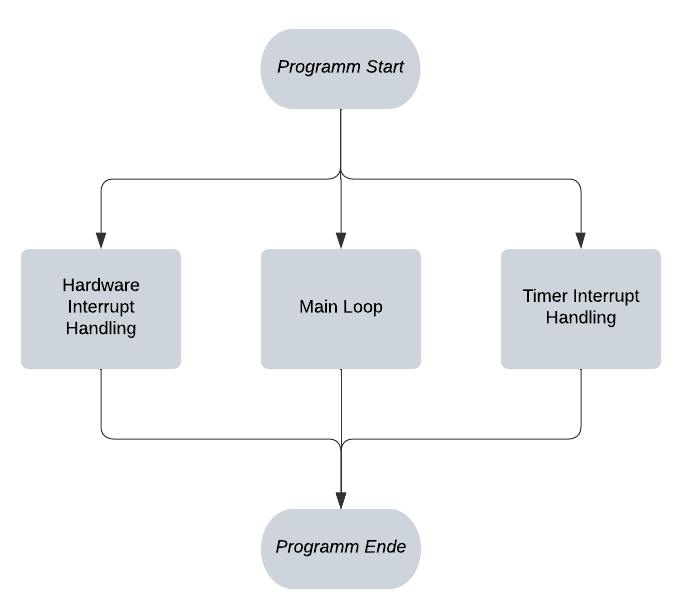
\includegraphics[width=8cm]{Bilder/Concurency.PNG}
\caption{Prozess-Parallelität}
\label{concur}
\end{center}
\end{figure}
\newpage
\section{Prozesse \& Softwarearchitektur}
Das gesamte Programm wird in vereinfachter Form durch drei parallel arbeitende Prozesse gesteuert: der \textbf{Main Loop}, den \textbf{Timer Interrupt} und den \textbf{Hardware Interrupt}. Diese Prozesse übernehmen unterschiedliche Aufgaben, um eine effiziente und stabile Steuerung sicherzustellen.\\

\paragraph{\textbf{1. Der Hardware Interrupt}} wird für zeitkritische Ereignisse verwendet und reagiert unmittelbar auf bestimmte Signale. Diese Funktionen beinhalten:
Interpretation der Motor-Hall-Sensoren (Ermittlung der Motorposition)
Erkennung des Hinterrad-Bremshebels (Einleitung des Bremsvorgangs)
Verarbeitung des Hardware Fault Signals (Kritische Fehlererkennung).\\
\paragraph{\textbf{2. Der Timer Interrupt}} arbeitet mit festen Zeitintervallen und dient der periodischen Ausführung zeitgesteuerter Aufgaben. Wie der Berechnung der Drehzahl (alle 100 ms), Übertragung von Daten an das Display (alle 500 ms), Software Fault Timeout (30s).
\begin{figure}[ht]
\begin{center}
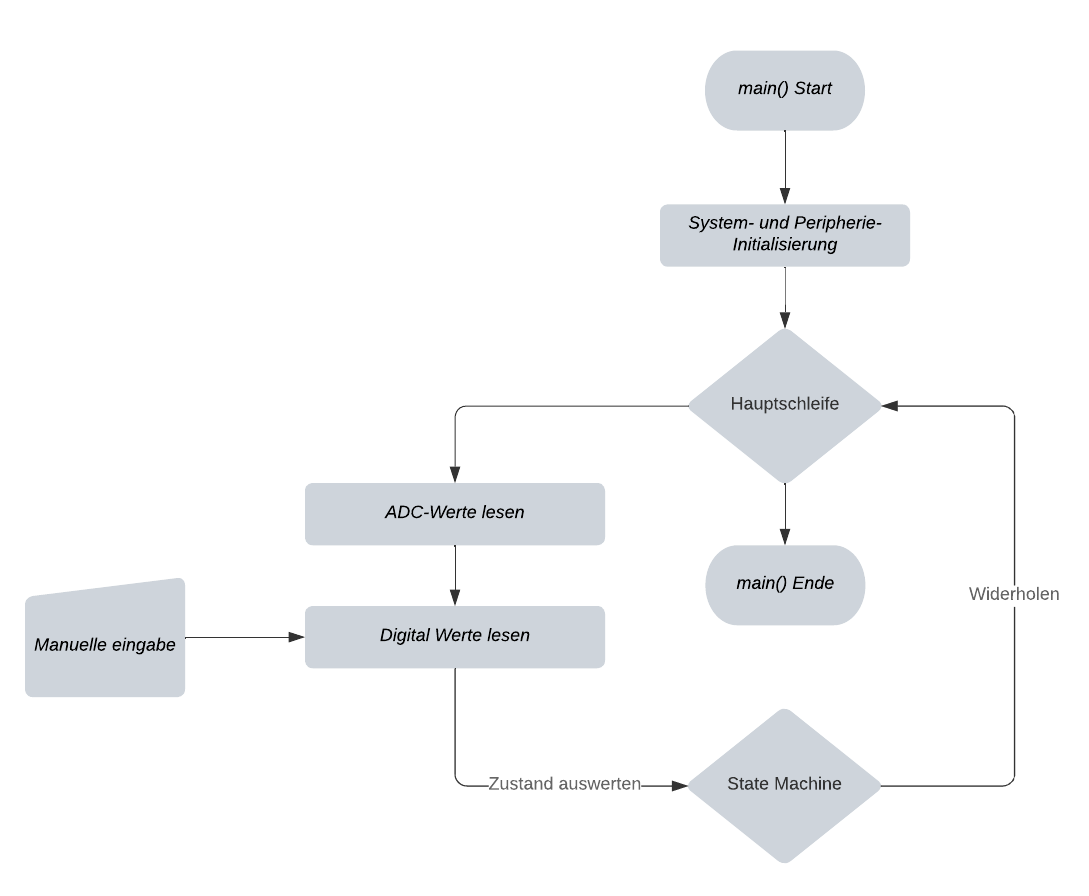
\includegraphics[width=8cm]{Bilder/mainLoop.PNG}
\caption{Ablauf-Diagramm Main Loop}
\label{mainl}
\end{center}
\end{figure}
\paragraph{\textbf{3. Die Main Loop}} bearbeitet zyklisch alle nicht zeitkritischen Aufgaben.
Dies beinhaltet: Einlesen\&Konvertieren der ADC-Messwerte, Abfrage der Bedientaster, Verarbeitung der Zustandsmaschine (State Machine), Setzen der digitalen Ausgänge (z. B. Beleuchtung, Lüftersteuerung).

\subsection{Zustandsautomat/State Machine}
Um die Vielzahl der Funktionen des Mikrocontrollers effizient und sicher zu verwalten, wurde in der Main Loop ein Zustandsautomat (State Machine) implementiert. Dieses Prinzip basiert auf der Definition von klaren Zuständen und Übergängen zwischen diesen, abhängig von bestimmten Bedingungen oder Ereignissen. Ein Zustandsautomat ist ein Kontrollflussmodell, das aus folgenden Elementen besteht:\\
\textbf{Zustände:} Definieren die aktuellen Betriebsmodi oder Aufgaben des Systems (z. B. Initialisierung, Normalbetrieb, Fehlerzustand).\\
\textbf{Übergänge:} Beschreiben die Bedingungen, unter denen das System von einem Zustand in einen anderen wechseln kann.\\
\textbf{Ereignisse oder Bedingungen:} Lösen die Übergänge zwischen Zuständen aus (z. B. Sensorwerte, Timer, Benutzereingaben).\\

\begin{figure}[ht]
\begin{center}
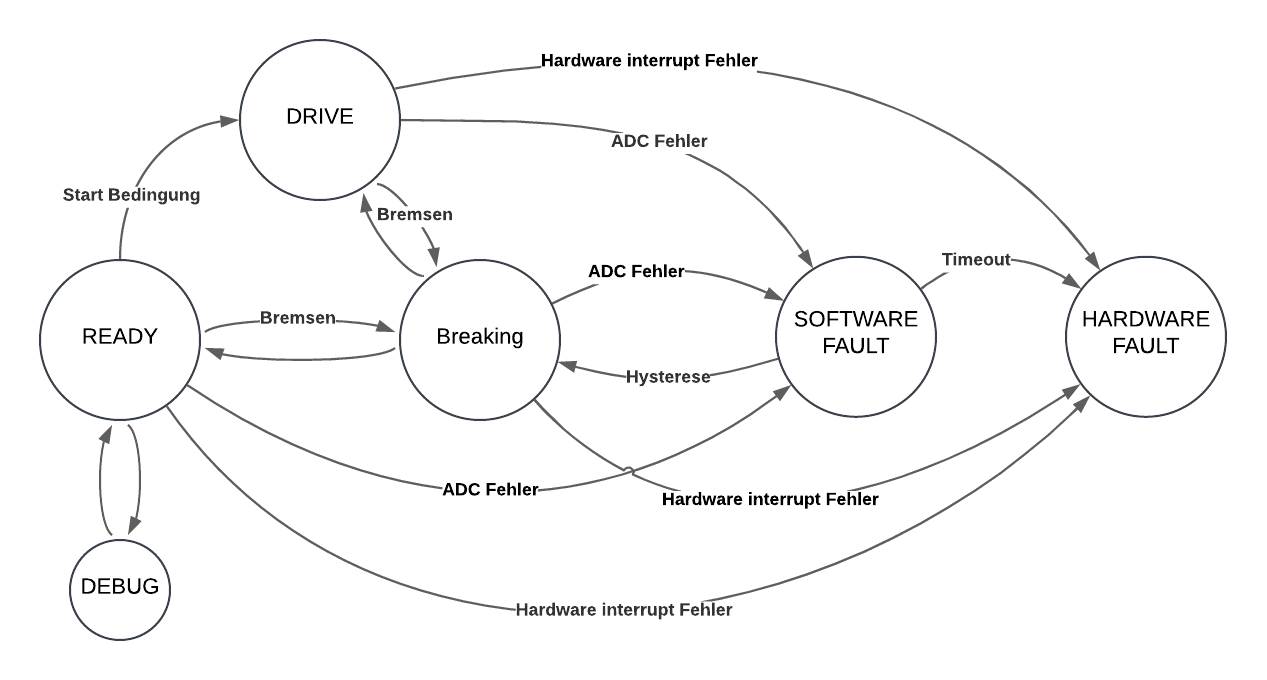
\includegraphics[width=16cm]{Bilder/AtomatenDiagramm.PNG}
\caption{Zustandsautomaten Diagramm}
\label{StateM}
\end{center}
\end{figure}
\newpage

Die in Abbildung \ref{StateM} dargestellten Zustände:\\
\textbf{READY:}\\
Nach Abschluss der Systeminitialisierung wechselt der Controller in den „Standby“-Zustand.
In diesem Zustand bietet das Geräte folgende Funktionen:
Steuerung der Beleuchtung,
Initialisierung des Motors,
Aktivierung der Lüfter bei Temperaturen (T) $\geq$ 60°C.\\
\textbf{DRIVE:}\\
Dieser Zustand repräsentiert den Fahrbetrieb. Mit den Funktionen:
Steuerung der Beleuchtung,
Volle Motorleistung,
Aktivierung der Lüfter bei T $\geq$ 60°C.\\
\textbf{BRAKING:}\\
Dieser Zustand repräsentiert das aktive Motorbremsen.
Zustandsfunktionen:
Steuerung der Beleuchtung,
Motor im Bremsbetrieb,
Aktivierung der Lüfter bei T $\geq$ 60°C.\\
\textbf{SOFTWARE FAULT:}\\
In diesem Zustand wird der Motor gestoppt, Beleuchtungselemente werden deaktiviert, um Last zu reduzieren.\\
\textbf{HARDWARE FAULT:}\\
Dieser Zustand gilt als kritisch, er kann nur durch Aus- und erneutes Einschalten des Geräts verlassen werden und Blockiert alle Funktionen wie Motor und Beleuchtung-Steuerung.
Optional kann das gerät sich selbstständig abschalten durch öffnen des Selbsthalterelais.\\
\\
Übergänge wie in Abbildung \ref{StateM} dargestellte:\\
\textbf{Start:}\\
Bedingung: Das Gerät befindet sich im READY-Zustand, Drehzahl = 0,
Der Nutzer drückt den Start-Taster oder bewegt den Gas-Griff, woraufhin das Gerät in den DRIVE-Zustand wechselt und die Fahrt beginnt.\\
\textbf{Bremsen:}\\
Der Nutzer betätigt während der Fahrt den Bremshebel, wodurch ein Hardware-Interrupt ausgelöst wird.
Der Motor wechselt vom Antriebsmodus in den Bremsmodus.
Sobald der Motor bis zum Stillstand abgebremst ist, wechselt das Gerät zurück in den READY-Zustand. Wird der Bremshebel losgelassen, bevor die Drehzahl 0 erreicht, kehrt das Gerät in den DRIVE Zustand zurück.\\
\textbf{ADC-Fehler:}\\
Tritt ein ADC-Messwert über einen definierten Grenzwert (z. B. Kühlkörpertemperatur > 100°C), betritt das System den SOFTWARE FAULT-Zustand. Dieser Zustand kann nur verlassen werden in dem die Temperatur wieder unter 80°C fällt. Dies passiert über den BRAKE Zustand, um versehentliches Start des Motors zu vermeiden.\\
\textbf{Timeout:}\\
Mit dem betreten des SOFTWARE FAULT Zustands wird ein 30s Timer gestartet, wenn dieser Zustand nicht vor ablaufen dieses Timers verlässt. Wechselt es den HARDWARE FAULT-Zustand.\\
\textbf{Hardware-Interrupt-Fehler:}
Beispiel Die Spannung Des Akkus fällt unter 42.9V löst die Hardware Messschaltung (siehe Schaltplan Abbildung \ref{UV}) aus und betätigt damit den Fault Interrupt-Pin (siehe Schaltplan Abbildung \ref{orGate}). 

\section{Source Code}
Um die Dokumentation kompakt und übersichtlich zu gestalten, konzentriert sich dieser Abschnitt ausschließlich auf die Funktionen des Mikrocontrollers, die für die Hauptlogik und Steuerung des Systems entscheidend sind. Allgemeine Quellcode-Elemente wie die Konfiguration von GPIOs, Timern oder Middleware werden bewusst vernachlässigt. Die hier erklärten Source Code ausschnitte finden sie im Anhang unter Source Code
\subsection{Main.c/h}
\paragraph{\textbf{Main Loop}} siehe Anhang Source Code~\ref{main}\\
implementiert eine Endlosschleife (while(1)), die eine Zustandsmaschine zur Steuerung verschiedener Betriebszustände verwendet. In jedem Schleifendurchlauf werden zunächst Eingaben durch readADCs(), readDI() erfasst und mit doADCs() setDO() verarbeitet. Anschließend wird ein switch-Statement basierend auf der aktuellen Systemzustandsvariable (STATE) ausgeführt. Je nach Zustand (READY, DRIVE, BREAK, etc) werden entsprechende Funktionen aufgerufen, um den Systemstatus zu verwalten, beispielsweise ready(). In fehlerhaften Zuständen (SWFAULT und HWFAULT) werden die digitalen Ausgänge (DO) mit resetDO() zurückgesetzt, während in regulären Betriebszuständen setDO() aktiviert wird. Zusätzlich wird ein LCD-Display alle 500 ms aktualisiert, wenn der Zähler timcc den Wert 5 erreicht. Am Ende jedes Schleifendurchlaufs wird eine Verzögerung von 25 ms mit HAL\_Delay(25); eingefügt, um den Prozessor zu entlasten.
\paragraph{\textbf{readADCs()}} siehe Anhang Source Code~\ref{readADC}\\
Die Funktion readADCs liest analoge Werte von drei unterschiedlichen Quellen (Spannung, Strom und Temperatur) ein und speichert die Ergebnisse in einem globalen Array ADC\_VAL.
\paragraph{\textbf{doADCs()}} siehe Anhang Source Code~\ref{doADC}\\
Die Funktion doADCs analysiert die erfassten ADC-Werte, überprüft Grenzwerte und steuert Systemkomponenten wie den Lüfter basierend auf den Messwerten. Sie verwaltet zudem Zustandsübergänge und erkennt Fehlerzustände.
\paragraph{\textbf{readDI()}} siehe Anhang Source Code~\ref{readDI}\\
Die Funktion readDI liest den Zustand von vier digitalen Eingängen (Tastern) ein und aktualisiert ein globales Array but, das diese Zustände speichert.
\paragraph{\textbf{setDO()}} siehe Anhang Source Code~\ref{setDO}\\
Die Funktion setDO setzt digitale Ausgänge basierend auf dem aktuellen Zustand der Taster (gespeichert im globalen Array but) und steuert damit Systemkomponenten wie Licht, Blinker und einen Debug-Modus.
\paragraph{\textbf{ready()}} siehe Anhang Source Code~\ref{ready}\\
Die Funktion ready prüft den Gasgriff und initialisiert den Motor, falls die Startbedingungen erfüllt sind. Wenn der Gasgriff eine bestimmte Schwelle überschreitet, wird das System in den Zustand DRIVE versetzt und der BLDC-Motor gestartet.
\paragraph{\textbf{drive()}} siehe Anhang Source Code~\ref{drive}\\
Die Funktion drive liest den Gasgriffwert ein, berechnet den entsprechenden Duty-Cycle und aktualisiert diesen, um die Motorgeschwindigkeit während des Fahrmodus zu steuern. Bei einem Fehler in der ADC-Konvertierung wird der Duty-Cycle auf einen sicheren Wert gesetzt, und ein Fehlerzustand ausgelöst.
\paragraph{\textbf{breaking()}} siehe Anhang Source Code~\ref{break}\\
Die Funktion breaking setzt den Motor in den Bremsmodus, indem sie die PWM-Signale stoppt und die Motorphasen kurzschließt, um die Bewegung zu verlangsamen oder zu stoppen
\paragraph{\textbf{swfault()}} siehe Anhang Source Code~\ref{swfault}\\
Die Funktion swfault wird aufgerufen, wenn ein Softwarefehler erkannt wird. Sie setzt das System in einen sicheren Zustand durch Aktivierung des Bremsmodus und überwacht, ob der Fehlerzustand über einen definierten Timeout hinaus anhält.
\paragraph{\textbf{hwfault()}} siehe Anhang Source Code~\ref{hwfault}\\
Die Funktion hwfault behandelt einen dauerhaften Hardwarefehlerzustand. Sie stoppt das System vollständig und zeigt eine Fehlermeldung an, während sie auf einen Neustart (Power-On-Reset) wartet.\\
\paragraph{\textbf{HAL\_GPIO\_EXTI\_Callback()}} siehe Anhang Source Code~\ref{interrupt}\\
Die Funktion HAL\_GPIO\_EXTI\_Callback wird aufgerufen, wenn ein externer GPIO-Interrupt ausgelöst wird. Sie verarbeitet verschiedene Arten von Interrupts, darunter Brems-, Hardwarefehler- und Hall-Sensor-Interrupts, abhängig vom Zustand des Systems und dem auslösenden Pin.\\
\paragraph{\textbf{handleHardwareFaultInterrupt()}} siehe Anhang Source Code~\ref{hwint}\\
Wechselt bei Hardwarefehlern in den entsprechenden Fehlerzustand. Optional: Fehlerdiagnose kann implementiert werden.
\paragraph{\textbf{handleBreakInterrupt()}} siehe Anhang Source Code~\ref{brint}\\
Die Funktion handleBreakInterrupt verarbeitet den Interrupt, der durch das Betätigen oder Loslassen des Bremshebels ausgelöst wird. Sie wechselt den Systemzustand zwischen BREAK und READY.
\paragraph{\textbf{handleHallSensorInterrupt()}} siehe Anhang Source Code~\ref{senint}\\
Die Funktion handleHallSensorInterrupt verarbeitet Interrupts, die durch Änderungen an den Hall-Sensoren ausgelöst werden. Sie zählt die Rotationsschritte des Motors, ermittelt die aktuelle Rotorposition und steuert die Motorphasen basierend auf trapezförmiger Kommutierung.

\subsection{BLDC.c/h}
\paragraph{\textbf{hallState()}} siehe Anhang Source Code~\ref{hallS}\\
Die Funktion hallState interpretiert die Zustände der Hall-Sensoren (ein Array mit drei Werten) und ermittelt die aktuelle Position des Rotors in Bezug auf die elektrische Kommutationsstufe (zwischen 0 und 5).
\paragraph{\textbf{commutator()}} siehe Anhang Source Code~\ref{commuta}\\
Die Funktion commutator steuert die drei Phasen eines BLDC-Motors basierend auf der Kommutatorposition, dem gewünschten Duty-Cycle (PWM-Signal) und der Drehrichtung des Motors.
\paragraph{\textbf{initBLDC()}} siehe Anhang Source Code~\ref{initBL}\\
Die Funktion initBLDC initialisiert den BLDC-Motor basierend auf den aktuellen Hall-Sensor-Zuständen.
\paragraph{\textbf{BLDCbreak()}} siehe Anhang Source Code~\ref{BLbreak}\\
Die Funktion BLDCbreak versetzt den BLDC-Motor in den Bremsmodus, indem sie alle Phasen des Motors kurzschließt und die PWM-Ausgabe deaktiviert.
\subsection{liquidcrystal\_i2c.c/h}
\paragraph{\textbf{lcd struct}} siehe Anhang Source Code~\ref{struct}\\
Die Struktur lcd\_ar wird verwendet, um Daten und Cursorpositionen für die Aktualisierung eines LCD-Displays zu speichern. Sie enthält die wichtigsten Systemparameter sowie deren Positionen auf dem Display.
\paragraph{\textbf{HD44780\_SetCursor()}} siehe Anhang Source Code~\ref{setC}\\
Die Funktion HD44780\_SetCursor setzt die Position des Cursors auf einem HD44780-kompatiblen LCD-Display. Die Position wird durch die Spalte (col) und die Zeile (row) angegeben.
\paragraph{\textbf{HD44780\_PrintStr()}} siehe Anhang Source Code~\ref{print}\\
Die Funktion HD44780\_PrintStr schreibt eine Zeichenkette (String) auf ein HD44780-kompatibles LCD-Display.
\paragraph{\textbf{Init\_lcd\_ar()}} siehe Anhang Source Code~\ref{initLCD}\\
Die Funktion Init\_lcd\_ar initialisiert eine Instanz der Struktur lcd\_ar mit Standard-Cursor-Positionen und voreingestellten Anzeigewerten auf einem HD44780-kompatiblen LCD-Display.
\paragraph{\textbf{update\_lcd\_val()}} siehe Anhang Source Code~\ref{upLCD}\\
Die Funktion update\_lcd\_val aktualisiert sowohl die Daten in einer lcd\_ar-Struktur als auch die Anzeige auf einem HD44780-kompatiblen LCD-Display mit neuen Sensorwerten.
\subsection{Mymath.c/h}
\paragraph{\textbf{pid struct}} siehe Anhang Source Code~\ref{pid}\\
Die Struktur pid\_f\_t wird verwendet, um die Parameter und Zustandsvariablen eines PID-Reglers (Proportional-Integral-Differential-Regler) zu speichern.\\
\paragraph{\textbf{map()}} siehe Anhang Source Code~\ref{map}\\
Die Funktion map skaliert einen Wert aus einem Bereich (Eingabebereich) in einen anderen Bereich (Zielbereich). Dies wird häufig verwendet, um Werte zwischen unterschiedlichen Skalen umzuwandeln, z. B. ADC-Werte in eine PWM-Skala.\\
\textbf{Formel:}\\ $mapped value = (\frac{x-in_{ min }}{in_{ max }-in_{ min }  })\times (out_{ max }-out_{ min })+out_{ min }$
\paragraph{\textbf{adc\_volt()}} siehe Anhang Source Code~\ref{adcV}\\
Die Funktion adc\_volt berechnet die Eingangsspannung (Vin) basierend auf einem Rohwert des ADC (val). Sie verwendet ein Spannungsteiler-Netzwerk, um die tatsächliche Spannung am Eingang zu bestimmen.\\
\textbf{Formel:}\\ $V_{ adc } = \frac{ val }{ 4095 } \times V_{ cc }$ ; $V_{in} = V_{adc} \times \left( \frac{R_1 + R_2}{R_2} \right)$
\paragraph{\textbf{adc\_cur()}} siehe Anhang Source Code~\ref{adcC}\\
Die Funktion adc\_cur berechnet den Strom in Ampere basierend auf einem Rohwert des ADC (val), einem Shunt-Widerstand und einem Verstärkungsfaktor.\\
\textbf{Formel:}\\ $V_{ adc } = \frac{ val }{ 4095 } \times V_{ cc }$ ; $V_{\text{adc\_adjusted}} = V_{\text{adc}} - 1,65V$ ; $V_{\text{shunt}} = \frac{V_{\text{adc\_adjusted}}}{\text{amplification\_factor}}$ ; $\text{current} = \frac{V_{\text{shunt}}}{R_{\text{shunt}}}$
\paragraph{\textbf{adc\_temp()}} siehe Anhang Source Code~\ref{adcT}\\
Die Funktion adc\_temp berechnet die Temperatur in Grad Celsius basierend auf einem Rohwert des ADC (val), der Spannungsteilerkonfiguration eines NTC-Thermistors (R1) und der Steinhart-Hart-Gleichung (vereinfachte Form mit Beta-Parameter).\\
\textbf{Formel:}\\ $V_{ adc } = \frac{ val }{ 4095 } \times V_{ cc }$ ; $R_1 = R_2 \times \left( \frac{V_{cc}}{V_{\text{adc}}} - 1.0 \right)$ ; $T = \frac{ 1.0 }{\frac{ 1 }{ T_{ 0 } } + \frac{ 1 }{ B } \times 1og(\frac{ R1 }{ R0 }) }$
\paragraph{\textbf{rpm\_tokmh()}} siehe Anhang Source Code~\ref{kmh}\\
Die Funktion rpm\_tokmh berechnet die Geschwindigkeit in Kilometern pro Stunde (km/h) basierend auf der Motordrehzahl (RPM) und dem Radumfang(U).\\
\textbf{Formel:}\\ $m/min = RPM \times U$; $kmh = \frac{ m/min \times 60min }{ 1000m }$
\subsection{stm32f4xx\_it.c/h}
\paragraph{\textbf{TIM2\_IRQHandler()}} siehe Anhang Source Code~\ref{tim2}\\
Die Funktion TIM2\_IRQHandler ist der Interrupt-Handler für den Timer TIM2, der mit einer Frequenz von 100 ms ausgelöst wird. Sie führt mehrere systemkritische Aufgaben aus, einschließlich der Berechnung der Drehzahl (RPM) und Geschwindigkeit sowie der Verwaltung von Zeitmessungen und Zuständen. Motor Sensor interrupt zähler (hallCC), Motor Polpaare (24).\\
\textbf{Formel:}\\
$x = hallCC \times 10 $ ; $rev = \frac{x}{24}$ ; $RPM = rev \times 60$
\newpage
\section{Controller Konfiguration}
Controller Pinning und Konfiguration basiert auf dem opensource VESC 6.4 Schaltplan und wurden mit Hilfe des STM32CubeIDE Configuratos erweitert.
\begin{figure}[ht]
\begin{center}
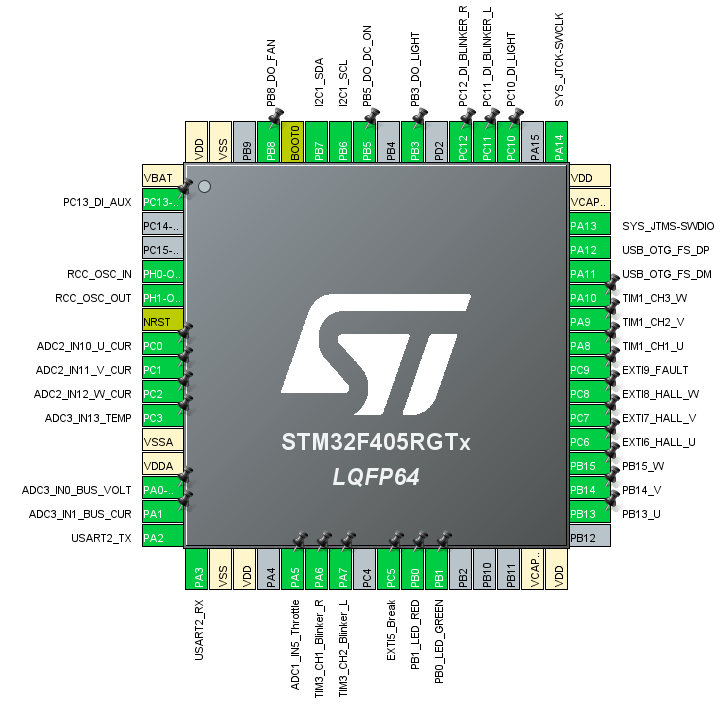
\includegraphics[width=14cm]{Bilder/ControlerConfig.PNG}
\caption{Pin Konfiguration}
\label{pinning}
\end{center}
\end{figure}

\begin{figure}[ht]
\begin{center}
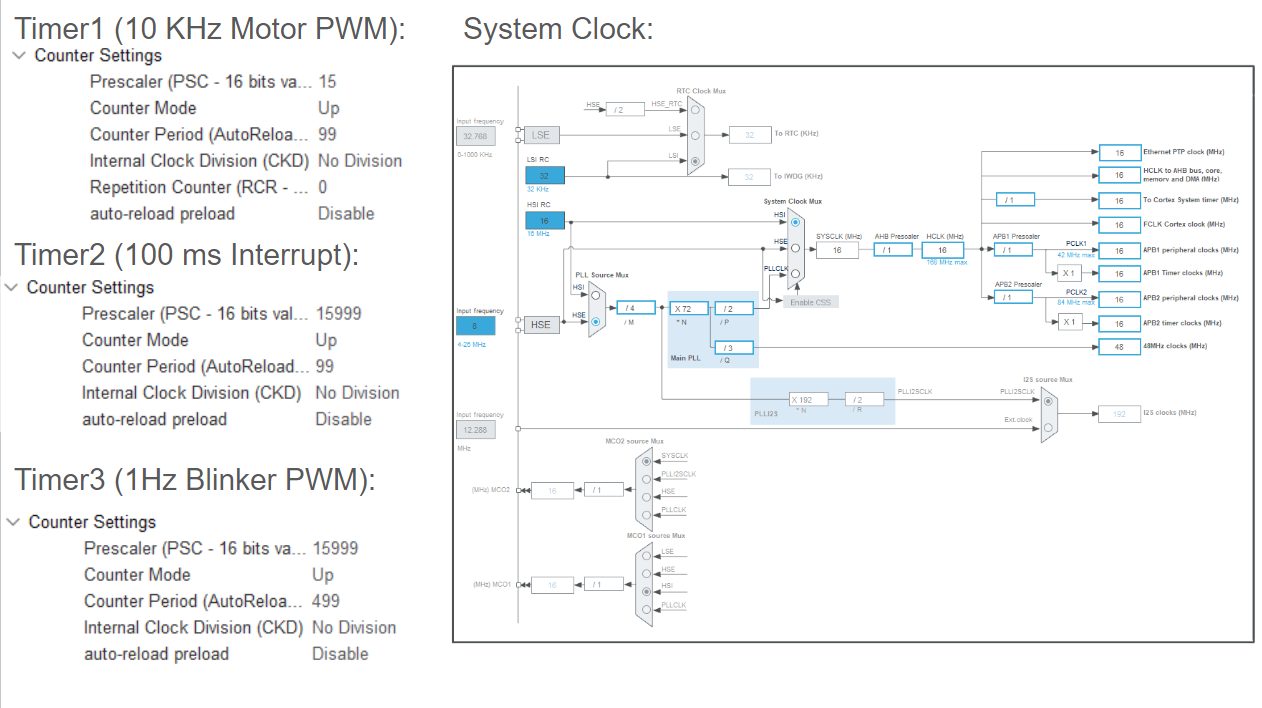
\includegraphics[angle=90,width=14cm]{Bilder/Timer.PNG}
\caption{System Clock Konfiguration}
\label{clock}
\end{center}
\end{figure}


\chapter{Gehäuse}
Die STL-Dateien der Gehäuse sind auf der Projekt-GitHub-Repository
github.com/leonreeh/E-Bike-ECU $\Rightarrow$ Gehäuse STL verfügbar. 
\begin{figure}[ht]
\begin{center}
\includegraphics[width=10cm]{Bilder/Gehäuse.PNG}
\caption{Gehäuse}
\label{Gehäuse}
\end{center}
\end{figure}
\section{Mechanische Eigenschaften}
\textbf{Material:} ASA (Acrylnitril-Styrol-Acrylat) wurde aufgrund seiner robusten mechanischen Eigenschaften gewählt. Es bietet hohe Temperatur- und UV-Beständigkeit und lässt sich einfach weiterverarbeiten. Das Material ist besonders geeignet für Anwendungen, die ständiger Witterung oder mechanischer Belastung ausgesetzt sind.\\
\textbf{Dimensionen:} Die Außenmaße betragen 272 × 140 × 77 mm, was ausreichend Platz für die notwendigen Elektronikkomponenten bietet und eine kompakte Integration ermöglicht.
\newpage
\section{Konstruktion}
Das Gehäuse besteht aus vier modularen Einzelteilen:
\textbf{Platinenträger:} Hier wird die elktronik mit hilfe von M3 schrauben befestigt
\textbf{Vorder- und Rückseite:} Diese Teile werden mithilfe von 3 × 60 mm Nägeln und einem speziellen ASA-Kleber dauerhaft mit dem Platinenträger verbunden. Dies sorgt für eine robuste und langanhaltende Fixierung.
\textbf{Deckel:} Der Deckel wird mit M4-Schrauben befestigt, was einen einfachen Zugriff auf die Elektronik bei Wartungsarbeiten ermöglicht.\\
Zur Anbindung von verschraubbaren Teilen werden sogenannte \textbf{Heatset-Inserts} verwendet. Diese bestehen aus Messing und können mithilfe eines Lötkolbens in das Kunststoffmaterial eingebracht werden. Dadurch entsteht ein langlebiges und stabiles Metallgewinde, das sich ideal für wiederholtes Verschrauben eignet.
M4 Inserts: Zum sicheren Verschrauben des Deckels.
M3 Inserts: Für die Montage der Platine und Lüfter.
\section{Gehäuse Komponenten}
\begin{figure}[ht]
\begin{center}
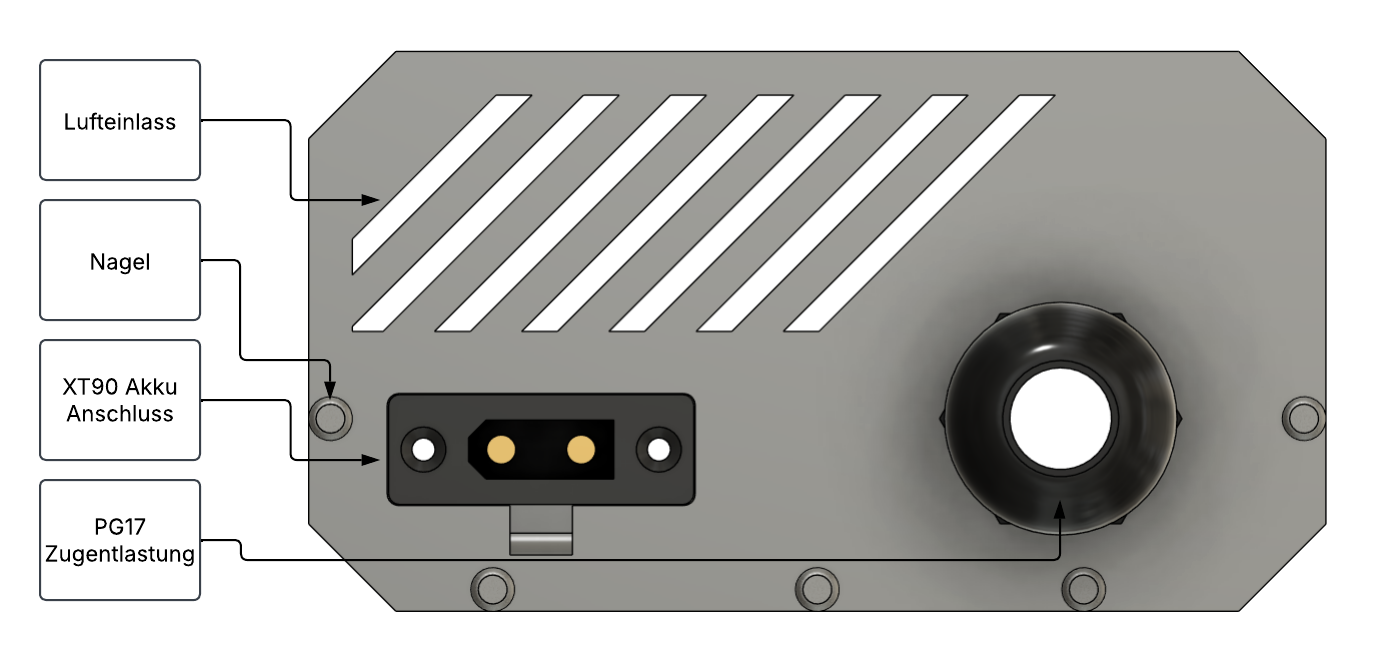
\includegraphics[width=12cm]{Bilder/FrontA.PNG}
\caption{Front}
\label{Front}
\end{center}
\end{figure}
Lufteinlässe: Passive Kühlung durch strategisch platzierte Lufteinlässe für optimale Wärmeableitung.
Anschlussbuchse: Eine XT90-Buchse dient zur Verbindung mit dem Akku. Diese ist für hohe Ströme ausgelegt und sorgt für sichere Energieübertragung.
Kabelzugentlastung: Eine PG17-Zugentlastung stellt sicher, dass die Leitungen für Bedienelemente und das Display sicher fixiert sind und keine mechanischen Belastungen auf die internen Verbindungen wirken.
Befestigung: Die Frontseite wird mit 5 Nägeln am Platinenträger montiert.
\newpage
\begin{figure}[ht]
\begin{center}
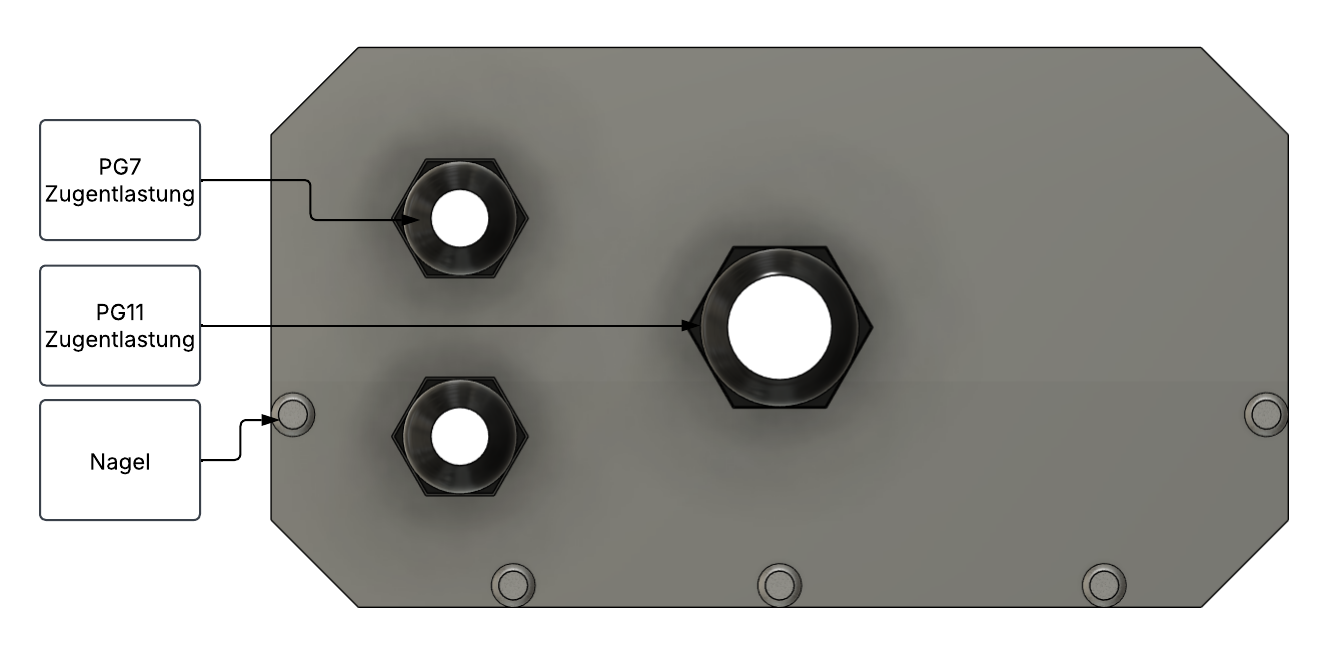
\includegraphics[width=12cm]{Bilder/BackA.PNG}
\caption{Rückseite}
\label{back}
\end{center}
\end{figure}
Kabelzugentlastungen:
PG11 für die Motorleitungen,
PG7 für die Heckbeleuchtung,
PG7 für die Heckblinker,
Befestigung: Auch die Rückseite wird mit 5 Nägeln sicher am Platinenträger fixiert.
\begin{figure}[ht]
\begin{center}
\includegraphics[width=10cm]{Bilder/botA.PNG}
\caption{Platinenträger}
\label{pholder}
\end{center}
\end{figure}
Heatset Inserts: M4 Inserts für die Montage des Deckels, M3 Inserts für die sichere Befestigung der Platine.
PCB-Standoffs: Integrierte PCB-Standoffs sorgen für zusätzliche Stabilität und unterstützen die Elektronik gegen Verbiegen. Diese Konstruktion minimiert mechanische Belastungen auf die Platine.
\newpage
\begin{figure}[ht]
\begin{center}
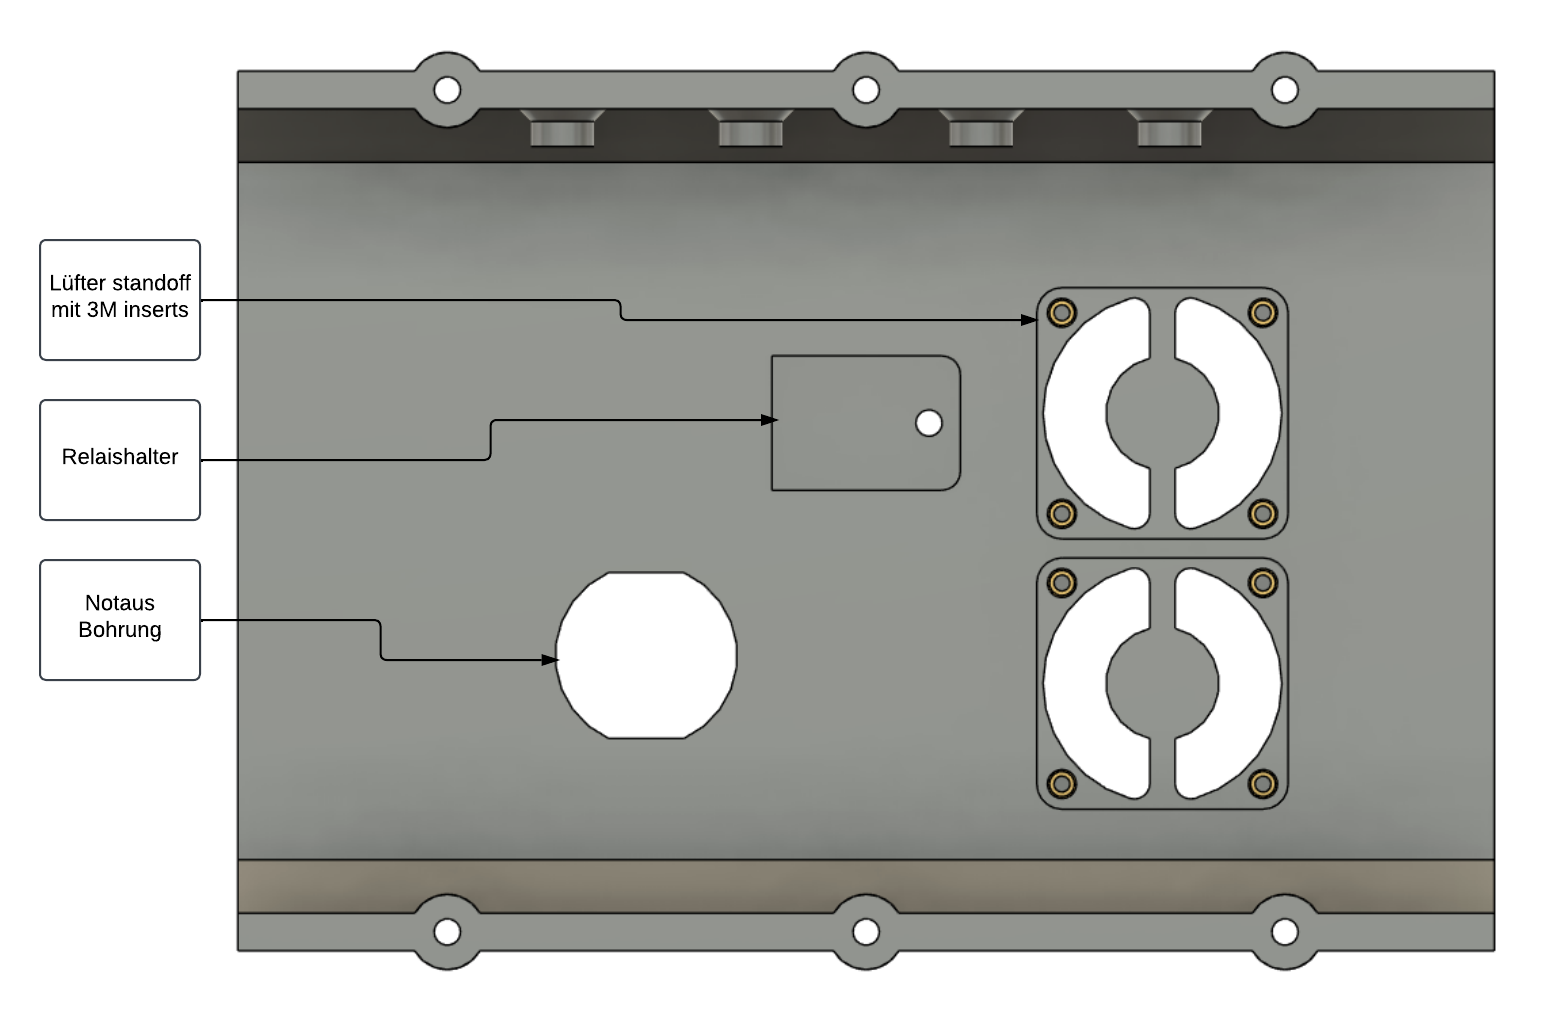
\includegraphics[width=10cm]{Bilder/Deckel.PNG}
\caption{Deckel}
\label{Deckel}
\end{center}
\end{figure}
Lüfter-Standoff: Ein erhöhter Bereich zur direkten Positionierung eines Lüfters über dem Kühlkörper, um die Wärmeableitung zu verbessern.
Relaishalter: Speziell designet Aussparungen sorgen für die sichere Positionierung und Fixierung des Relais.
Befestigungsbohrung: Eine Bohrung mit Registrierung ermöglicht die Montage eines Not-Aus-Schalters an einer zugänglichen Stelle.\\
\\
\textbf{Gehäuse Stückliste:}\\
\\
\begin{tabular}[h]{l|c|r}
\label{GeStk}
\textbf{Name} & \textbf{Stückzahl} & \textbf{Beschreibung} \\
\hline
Platinenträger & 1 & STL file für 3D druck \\
\hline
Deckel & 1 & STL file für 3D druck \\
\hline
Front & 1 & STL file für 3D druck \\
\hline
Rückseite & 1 & STL file für 3D druck \\
\hline
M3S Gewindeeinsatz & 20 & M3 gewinde insert \\
\hline
M4 Gewindeeinsatz & 6 & M4 gewinde insert \\
\hline
XT90E-M & 1 & Hochstrom Einbaustecker \\
\hline
PG17 & 1 & Zugentlastung \\
\hline
PG11 & 1 & Zugentlastung \\
\hline
PG7 & 2 & Zugentlastung \\
\end{tabular}



\part{Entwicklungsprozess und Relevante Konzepte}
In diesem Kapitel widme ich mich dem \textbf{Entwicklungsprozess} und den \textbf{relevanten Konzepten}, die für die Realisierung des Projekts von zentraler Bedeutung sind. Ziel ist es, einen Einblick in die methodische Herangehensweise und die zugrunde liegenden Entscheidungen zu geben, die den Weg von der ersten Idee bis hin zu einem funktionalen Prototypen geebnet haben.\\
Der Entwicklungsprozess folgt einer klar strukturierten Methodik – von der Planung über die Designphase bis hin zur Umsetzung. Zentrale Herausforderungen, wie die Auswahl geeigneter Hardware-Komponenten und die Entwicklung eines zuverlässigen Steuerungssystems, wurden durch einen systematischen Ansatz und eine speziell auf das Projekt zugeschnittene Strategie bewältigt. Dabei wurde das komplexe Gesamtsystem in kleinste funktionale Einheiten unterteilt, die in einzelnen Entwicklungsphasen überprüft wurden. Ziel war es, Designfehler frühzeitig zu erkennen und die Integration in das Gesamtsystem zu erleichtern.
\chapter{Entwicklungsprozess}
\paragraph{Planung}
Nach der Auswahl des Projektthemas begann die Recherche zu den grundlegenden Aspekten des E-Bikes. Wesentliche Fragestellungen, die beantwortet werden mussten, waren:\\
\textbf{Welcher Motor und wie wird er angesteuert?\\}
Im Bereich der E-Mobilität ist die Wahl der Motorart eindeutig: Der B\textbf{rushless DC Motor (BLDC)}. Aufgrund seines wartungsfreien Designs und seiner hohen Leistungsdichte eignet er sich ideal für Antriebssysteme und wird in verschiedensten Anwendungen von E-Bikes bis hin zu Elektroautos eingesetzt.\\
Für dieses Projekt fiel die Entscheidung auf einen diskreten BLDC-Hub-Motor. Ein Hub-Motor ist direkt in der Radnabe integriert, wodurch keine Änderungen am Fahrradrahmen erforderlich sind. Diese Bauweise erleichtert die Integration in bestehende Fahrräder erheblich. Zudem wird der Kettenantrieb des Fahrrads nicht belastet, da die Kraftübertragung direkt über das Rad erfolgt.\\
\textbf{Welcher Akku wird verwendet?\\}
Die am häufigsten in E-Bikes vertretenen Akkusysteme sind 7S (24V), 9S (32V) und 13S (48V). Mit einer Zielsetzung von 1 kW Leistung fiel die Wahl auf ein 48V-System. Diese Entscheidung ermöglicht es, den Stromfluss gering zu halten und dadurch die ohmschen Verluste in Leitungen und Steckverbindungen zu minimieren.\\
Basierend auf dieser Spannung konnten erste Hardware-Anforderungen dimensioniert werden, beispielsweise der Eingangsspannungsbereich des Netzteils, um eine stabile und effiziente Energieversorgung sicherzustellen. Siehe Anhang Entwicklung \ref{stateofC}\\
\textbf{Welche Zusatzfunktionen?}\\
Zusätzliche Features wie Beleuchtung und ein Display sollten integriert werden, um den Funktionsumfang zu erweitern und die Benutzererfahrung zu verbessern.

\paragraph{Designphase}
Für die Motorsteuerung wurde das Open-Source-„VESC-Projekt“ als Basis gewählt. Dieses ist bekannt für seine robuste Hardware für Akku betriebene Antriebssysteme im Kilowatt Bereich, sowie eine breite und modulare Softwarearchitektur. Durch diese Entscheidung wurde eine der komplexesten Herausforderungen des Projekts – die Auswahl eines geeigneten Mikrocontrollers – erheblich erleichtert. Die Vielfalt an verfügbaren Mikrocontrollern, z. B. von Herstellern wie Renesas, STMicro und NXP, und die unterschiedlichen Spezifikationen wie Speichergröße, 16/32-Bit-Systeme, Anzahl von Interrupts und ADC-Pins, machten diese Entscheidung besonders anspruchsvoll.\\
Aus dem VESC 6.4-Referenzdesign wurde die Mikrocontroller-Auswahl sowie dessen Pinbelegung übernommen, während der restliche Schaltplan und die gesamte Software vollständig eigenständig entwickelt wurden.
\newpage
\begin{figure}[ht]
\begin{center}
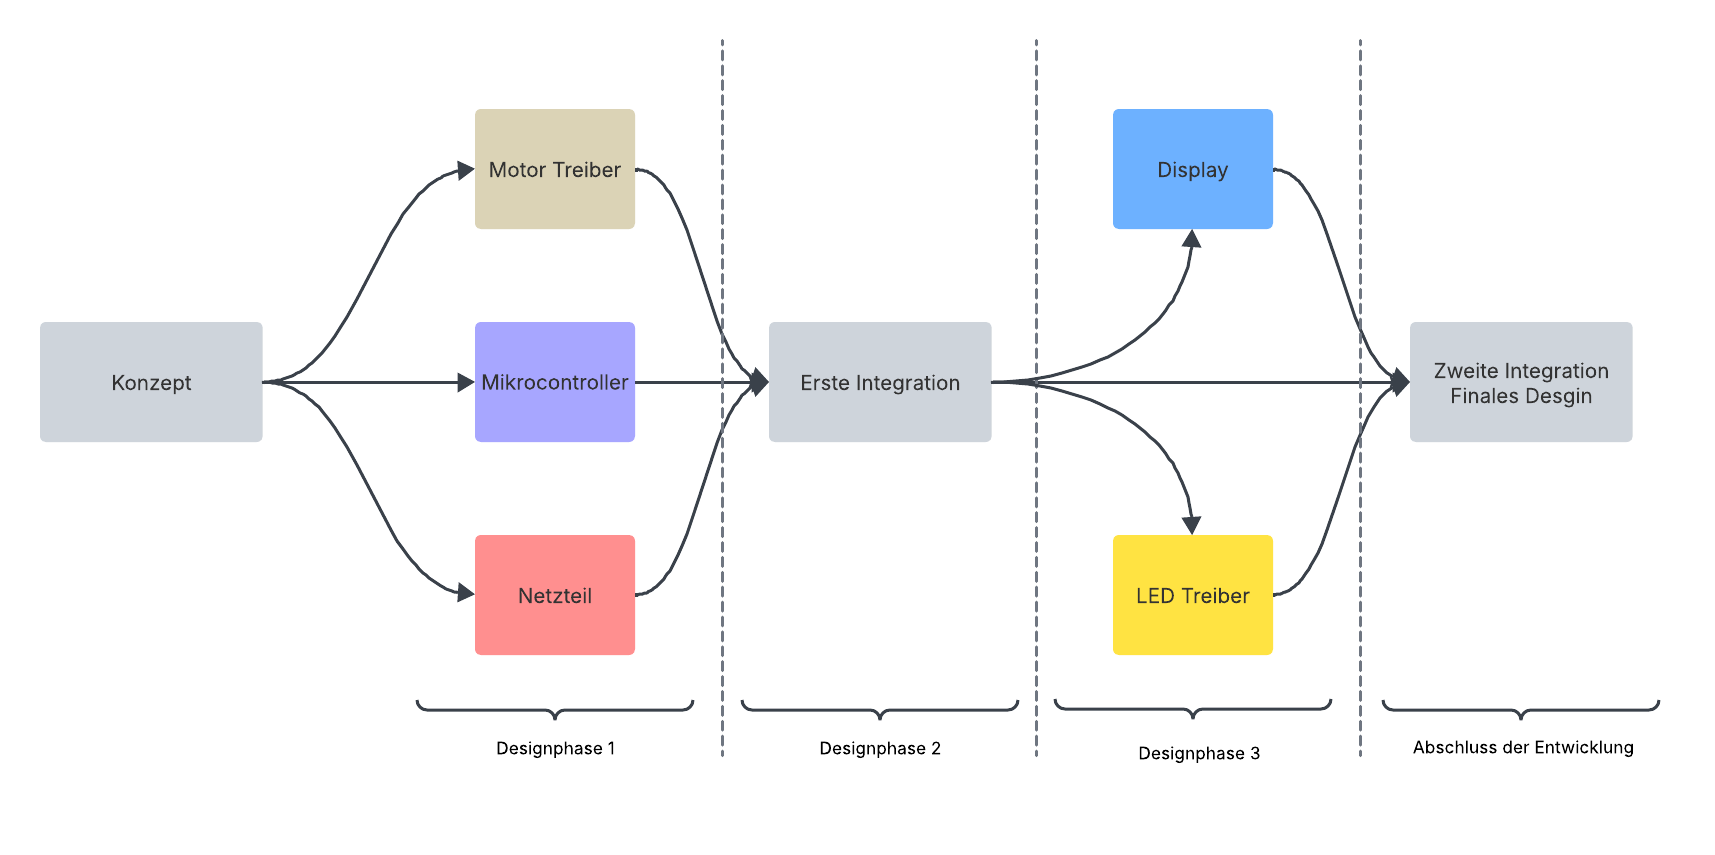
\includegraphics[angle=90,width=10cm]{Bilder/DesignPhase.PNG}
\caption{Designphasen}
\label{designp}
\end{center}
\end{figure}
\newpage
\chapter{Designphasen}
\section{Designphase 1}
\paragraph{Mikrocontroller}
Für die Inbetriebnahme des Mikrocontrollers wurde eine kompakte 2-Layer-Leiterplatte entworfen, die alle notwendigen Komponenten enthält, um eine funktionale und stabile Umgebung für die Softwareentwicklung zu gewährleisten. Die Leiterplatte umfasst:
\textbf{3.3V-Versorgung} zur Stromversorgung des Mikrocontrollers.
\textbf{Clock-Oszillator} für die Systemtaktung.
\textbf{Debug-LEDs}, die den Status oder Fehlerzustände anzeigen.
\textbf{Programmierschnittstelle}, um den Mikrocontroller mit der Entwicklungsumgebung zu verbinden.
\textbf{USB}-Debug-Kommunikation, die eine einfache Fehlersuche und Überwachung ermöglicht.
Lötpads für \textbf{GPIO-Anschlüsse}, um externe Komponenten flexibel verbinden zu können.\\
Diese Schaltung blieb über die gesamte Entwicklungsphase unverändert, da das Design von Anfang an stabil und zuverlässig lief.
\begin{figure}[ht]
\begin{center}
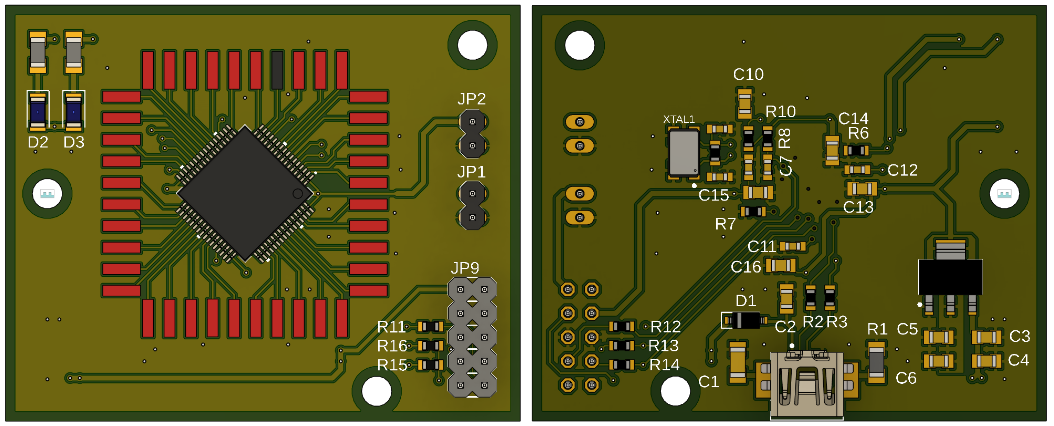
\includegraphics[width=10cm]{Bilder/MCU_EVL.PNG}
\caption{Designphasen}
\label{mcuevl}
\end{center}
\end{figure}
\paragraph{Motor Treiber}
Die Aufgabe des Motortreibers besteht in der Ansteuerung der drei BLDC-H-Brücken, der Phasenstrommessung für den Sinusbetrieb und der Drehmomentregelung. Die erste Version des Motortreibers basierte auf dem TI DRV8302 Treiber-IC, das aus dem VESC-Referenzdesign übernommen wurde. Dieses IC bot mehrere Vorteile: Integrierte \textbf{Spannungsversorgung} 12-60V. \textbf{Integrierte Verstärker} für die Phasenstrommessung. \textbf{Fehlererkennung} für Bootstrap-Spannung, Phasenstrom und Phasenspannung über Integrierte SPI Kommunikation. Einfache Integration durch ein gut dokumentiertes Design.
\newpage
\paragraph{Netzteil}
Das Netzteil übernimmt die Aufgabe, aus der Akku-Spannung von ~42–58V (siehe Anhang Entwicklung \ref{stateofC}) alle systemrelevanten Spannungen zu erzeugen:
12V (min. 1A): Versorgung von Beleuchtung, Lüftern und Relais.
5V (min. 0.5A): Stromquelle für das Display und die Motorsensoren.
3.3V (min. 0.3A): Energieversorgung für den Mikrocontroller und weitere logische Komponenten.\\
In der ersten Version des Netzteils wurde ein DC/DC-Spannungsregler für 12V und LDOs (Low-Dropout-Regler) für 5V und 3.3V verwendet. Die LDOs schienen aufgrund des geringen Beschaltungsaufwand eine kostengünstige Lösung zu sein.
Allerdings zeigten die Tests, dass der Spannungsabfall auf dem 5V-LDO zu hoch war, um die notwendige Leistung zuverlässig bereitzustellen. Dies führte zu einer Überarbeitung des Designs in Designphase 2.
\section{Designphase 2}
\paragraph{Integration}
Für die ersten Inbetriebnahmen wurde ein vereinfachter Testaufbau konzipiert, um die Funktion der einzelnen Baugruppen zu verifizieren und Schwachstellen im Design frühzeitig zu identifizieren.\\
Zur Sicherstellung des Personenschutzes kamen ein Labornetzteil mit Überstromschutz sowie ein kleiner, leistungsschwacher 50W NEMA-Motor zum Einsatz. Das Labornetzteil reduziert das Risiko elektrischer Fehler im Vergleich zur direkten Nutzung eines Akkus. Zudem minimiert der nur 300 g leichte Motor die Gefahren durch rotierende mechanische Teile im Vergleich zum deutlich leistungsstärkeren 36-Zoll-Hub-Motor.
\begin{figure}[ht]
\begin{center}
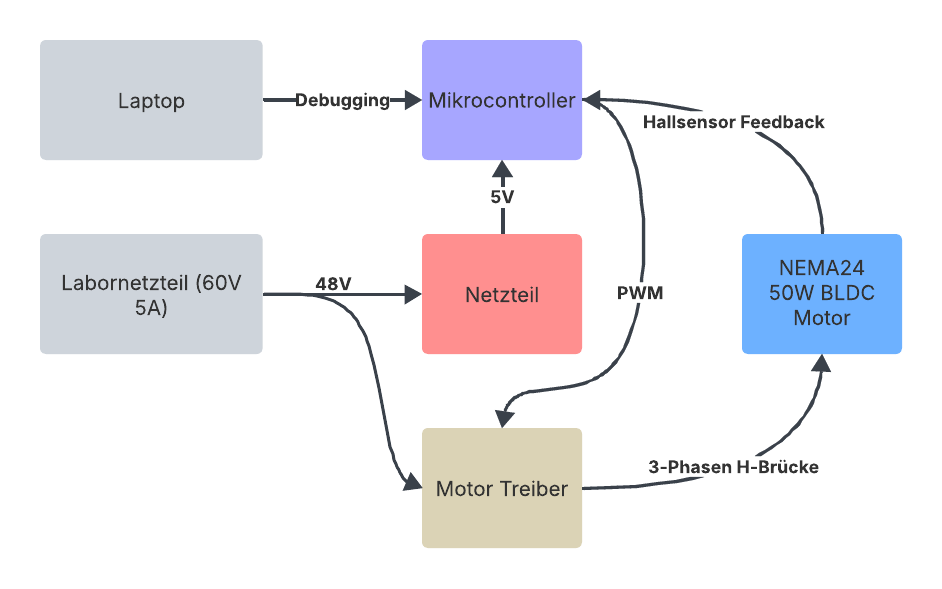
\includegraphics[width=12cm]{Bilder/Labortest.PNG}
\caption{Testaufbau Blockdiagramm}
\label{labtest}
\end{center}
\end{figure}
\newpage
\paragraph{Motor Treiber Redesign}
Trotz der Vorteile wurde der TI DRV8302 nicht für die finale Version verwendet, hauptsächlich aus folgenden Gründen: Hohe Kosten des Treiber-ICs (ca. 8 € pro Stück bei Distributoren wie Digikey).
Der Wunsch, das Design stärker von der Referenzlösung abzuheben und eigene Entwicklungen einzubringen.\\
In der zweiten Version wurde der Infineon IR2101S eingesetzt, ein Halbbrückenregler, der zu einem Bruchteil der Kosten (unter 1 €) erhältlich ist. Für die Phasenstrommessung war eine zusätzliche Verstärkerschaltung erforderlich, die mithilfe des AD8418 realisiert wurde. Dieses Design ermöglichte eine deutlich günstigere und individuellere Umsetzung.
\paragraph{Netzteil Redesign}
in der zweiten Version wurde der 5V-LDO durch einen weiteren DC/DC-Wandler ersetzt, um dessen Verluste zu minimieren. Hier für wurde ein neuer DC/DC-Wandler(LMR36520) mit variabler Ausgangsspannung eingeführt, um die selben Komponenten für 12V \& 5V Versorgung zu nutzen.
\section{Designphase 3}
Nachdem die grundlegenden Funktionen Gestalt angenommen hatten, konnten nun die Zusatzfunktionen in den Fokus genommen werden.
\paragraph{Display}
Für die Anbindung von Display-Modulen wurde eine spezielle bidirektionale Level-Shifter-Schaltung entwickelt (siehe Schaltplan Abbildung \ref{shifter}). Ziel war es, eine Schnittstelle zu schaffen, die das breite Angebot an Arduino-, ESP32- und Raspberry Pi-Displays voll ausnutzen kann. Dafür musste sowohl UART als auch I2C mit 3.3V- und 5V-Logik-Level unterstützt werden.\\
Es ist wichtig zu erwähnen, dass die verbaute Schaltung die Übertragungsrate auf die Schaltfrequenz des 2N7002-MOSFETs limitiert. Diese liegt mit rund 250 kHz jedoch weit über den benötigten 10–100 kHz (I2C Normal/Fast Speed) bzw. 9,6–115,2 kBaud (UART), die für herkömmliche Display-Module erforderlich sind. Das im finalen Design verwendete 2004 LCD benötigt lediglich 10 kHz I2C, sodass die gewählte Schaltung mehr als ausreichend ist.
\paragraph{LED Treiber}
Für die Steuerung der Beleuchtung war lediglich eine einfache MOSFET-Treiber-Schaltung erforderlich (siehe Schaltplan Abbildung \ref{blinker}). Diese konnte problemlos auf einer Lochrasterplatine evaluiert werden und ermöglicht die Ansteuerung gängiger 12V-Fahrrad- und Motorradbeleuchtungselemente.\\
Die gleiche Schaltung wurde zudem für den Betrieb der Lüfter sowie des Selbsthaltere­lais verwendet. Hier war lediglich die Ergänzung einer Freilaufdiode erforderlich, um Spannungsspitzen beim Schalten der induktiven Lasten zu vermeiden.
\newpage
\section{Abschluss der Entwicklung}
Nach der Fertigstellung der finalen Designs der einzelnen Funktionsgruppen wurde eine Gesamthardware entwickelt, die alle Komponenten nahtlos miteinander verbindet. Diese schrittweise Integration erwies sich als äußerst effizient, da sie mehrere Vorteile bot:\\
\textbf{Kostenersparnis:} Durch die Iteration auf kleinen, kostengünstigen 2-Layer-PCBs, die weniger Bestückungsaufwand erforderten.\\
\textbf{Zeitersparnis:} Die Integration basierte auf stabilen und getesteten Funktionsgruppen, wodurch bereits fertige Layouts einfach miteinander verbunden werden konnten.\\
\textbf{Erhöhte Zuverlässigkeit:} Potenzielle Fehlerquellen wurden bereits in der zweiten Designphase identifiziert und behoben, was die Robustheit der Gesamthardware deutlich verbesserte.\\
Die erfolgreiche Integration aller Funktionsgruppen in eine einzige, optimierte Hardware stellte somit einen entscheidenden Meilenstein in der Realisierung des Projekts dar.


\chapter{Relevante Konzepte}
\section{BLDC}
\paragraph{Grundlagen}
Ein BLDC-Motor (bürstenloser Gleichstrommotor) funktioniert durch ein rotierendes Magnetfeld, das von Spulen im Stator erzeugt wird. Der Rotor mit Permanentmagneten wird von diesem Magnetfeld angezogen und in Drehung versetzt.\\
\begin{figure}[ht]
\begin{center}
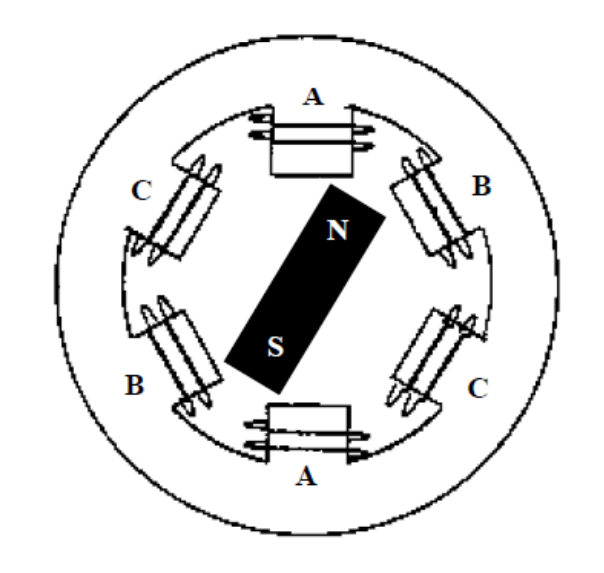
\includegraphics[width=8cm]{Bilder/Motor.PNG}
\caption{(Texas Instruments. (2015). Trapezoidal Control of BLDC Motors Using Hall Effect Sensors . C2000 Systems and Applications Team, Bilal Akin, Manish Bhardwaj, \& Jon Warriner.)}
\label{motor}
\end{center}
\end{figure}

Zur Synchronisation des elektrischen Stroms mit der Position des Rotors verwenden BLDC-Motoren häufig Hallsensoren oder andere Positionssensoren.
Diese Sensoren ermitteln die exakte Position des Rotors und geben diese Information an den Controller weiter, sodass die Spulen präzise im richtigen Moment angesteuert werden. Diese Sensorik machen einen der erheblichen vorteile von modernen BLDC motoren gegenüber herkömmlichen Wechselstrom motoren aus. 
\newpage
\paragraph{Ansteuerung}
Die Steuerung von BLDC-Motoren (Brushless DC-Motoren) ist ein zentraler Aspekt ihrer Anwendung und bestimmt maßgeblich die Effizienz, Laufruhe und Steuerbarkeit der Motoren. In diesem Kapitel werden die wichtigsten Steuerungsmethoden für BLDC-Motoren beschrieben: Sinussteuerung, FOC-Steuerung und Trapezsteuerung.
\paragraph{Trapez Steuerung} ist eine einfachere und kostengünstigere Methode zur Steuerung von BLDC-Motoren. Sie verwendet rechteckige (trapezförmige) Spannungs- oder Stromwellen, um die Phasen des Motors zu betreiben.\textbf{Funktionsweise:}
Der Rotor wird durch das Erzeugen eines trapezförmigen Magnetfelds angetrieben. Die Kommutierung erfolgt diskret in Schritten von 60° elektrischem Winkel. Die Rotorposition wird meist mithilfe von Hall-Sensoren erfasst. \textbf{Vorteile:}
Einfache Umsetzung, Hohes Drehmoment, Geringste Schaltverluste,
\textbf{Nachteile:} Höhere Geräusch- und Vibrationsentwicklung im Vergleich zu Sinus- oder FOC-Steuerung. Weniger effizient, besonders bei hoher Drehzahl.
\begin{figure}[ht]
\begin{center}
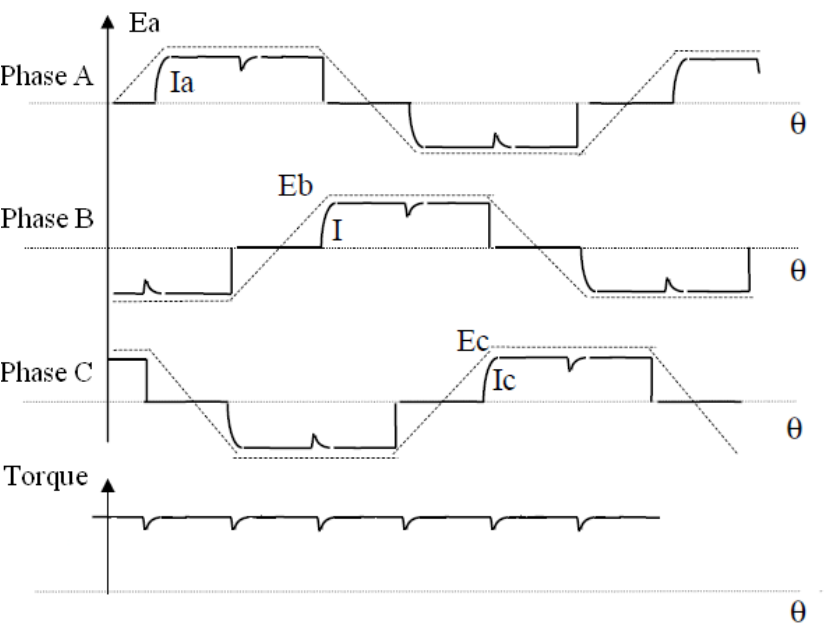
\includegraphics[width=8cm]{Bilder/trap.PNG}
\caption{(Texas Instruments. (2015). Trapezoidal Control of BLDC Motors Using Hall Effect Sensors . C2000 Systems and Applications Team, Bilal Akin, Manish Bhardwaj, \& Jon Warriner.)}
\label{trap}
\end{center}
\end{figure}
\paragraph{Sinus Steuerung} basiert darauf, die Ströme in den Phasen des Motors so zu regeln, dass sie sinusförmig verlaufen. Dadurch wird ein gleichmäßiges Drehmoment erzeugt, was sich in einer hohen Laufruhe und geringen Vibrationen äußert. \textbf{Funktionsweise:}
Die Sinussteuerung verwendet Sinuswellen als Referenzsignal für die Phasenströme. Diese werden über Pulsweitenmodulation (PWM) in die Wicklungen eingespeist. \textbf{Vorteile:} Sehr leiser und vibrationsarmer Betrieb. Bessere Effizienz bei hohen Drehzahlen. Geeignet für Anwendungen, bei denen Laufruhe entscheidend ist. \textbf{Nachteile:} Erfordert komplexe Elektronik und präzise Sensorik zur Bestimmung der Rotorposition. Kann weniger effizient sein als andere Methoden bei hoher Last im unteren Drehzahl-Bereich.
\paragraph{FOC Steuerung} Field-Oriented Control (Vektorregelung) ist eine fortschrittliche Methode zur Steuerung von BLDC-Motoren. Sie nutzt mathematische Transformationen, um die Drehmoment- und Magnetisierungsströme unabhängig voneinander zu regeln. \textbf{Funktionsweise:} Die Rotorposition wird kontinuierlich überwacht, oft mithilfe von Hall-Sensoren oder Encodern. Mithilfe einer Park- und Clarke-Transformation werden die Phasenströme von einem dreiphasigen in ein zweidimensionales Koordinatensystem (d-q-Achsen) transformiert. Dies ermöglicht die gezielte Regelung des Drehmoments (q-Achse) und der Magnetisierung (d-Achse). \textbf{Vorteile:} Sehr hohe Effizienz bei variabler Drehzahl und Last. Präzise Steuerung des Drehmoments. Unterstützt hohe Drehzahlen und bietet bessere Leistung als andere Methoden. \textbf{Nachteile:} Hohe Rechenleistung erforderlich, da fortschrittliche Algorithmen verwendet werden. Aufwendige Sensorik und Kalibrierung notwendig.
\paragraph{}In diesem Projekt wurde die Trapezsteuerung als Steuerungsmethode ausgewählt. Ausschlaggebend hierfür waren die einfache Implementierung, das hohe Drehmoment und die vorhandene Sensorik des Fahrradmotors, der nur eine Auflösung von 60° bietet. Die Hardware des Systems ist jedoch vollständig ausgestattet, um auch eine Sinussteuerung zu realisieren. Eine Umsetzung der FOC-Steuerung ist hingegen mit dem aktuellen Motor nicht möglich, da hierfür entweder präzisere Hall-Sensoren oder eine Back-EMF-Messschaltung erforderlich wären.
\part{Anhang}

\chapter{System Design}
\textbf{System Komponenten:}\\
\\
\begin{tabular}[h]{l|c|r}
\label{SysKomp}
\textbf{Bauteil} & \textbf{Name} & \textbf{Beschreibung} \\
\hline
Motor & Viribus LY23048911 & 1KW BLDC Motor \\
\hline
Akku & Unit Pack S039-3 & 48V 15Ah 750W/h\\
\hline
Display & GeeekPi I2C 2004 LCD & 20x4 LCD I²C display\\
\hline
 & QWork WD7435 & Lenkerschalter-Beleucht\\  
Bedienelemte & Greluma ZL277LUM & Lenker E-Stop Schalter\\
 & VGEBY B08KFC114S & Analog Gasgriff\\
 \hline
Scheinwerfer & Filmer 49002 & Fahrad Scheinwerfer\\
\hline
Rücklicht & evermotor A08051-3 & Motorrad 50mm Brems-Rücklicht\\
\hline
Blinker & Dowrap B0CK6ZTGS3 & 12V Led blinker Vorne\\
 & evermotor A08023 & 12V Led blinker Hinten\\
\hline
Steuergerät & RESC\_V2 & 13-64V 30A E-Bike Steuergerät\\
\hline
Notaus & Tawvelm SPST & 48V 100A DC Schalter\\
\hline
Lüfter & 2x GDA4010 & 40x10mm 12V Lüfter\\
\hline
Kühlkörper & VPR138/94-M3 & 94x46x33mm Kühlkörper\\
\end{tabular}

\begin{figure}[ht]
\begin{center}
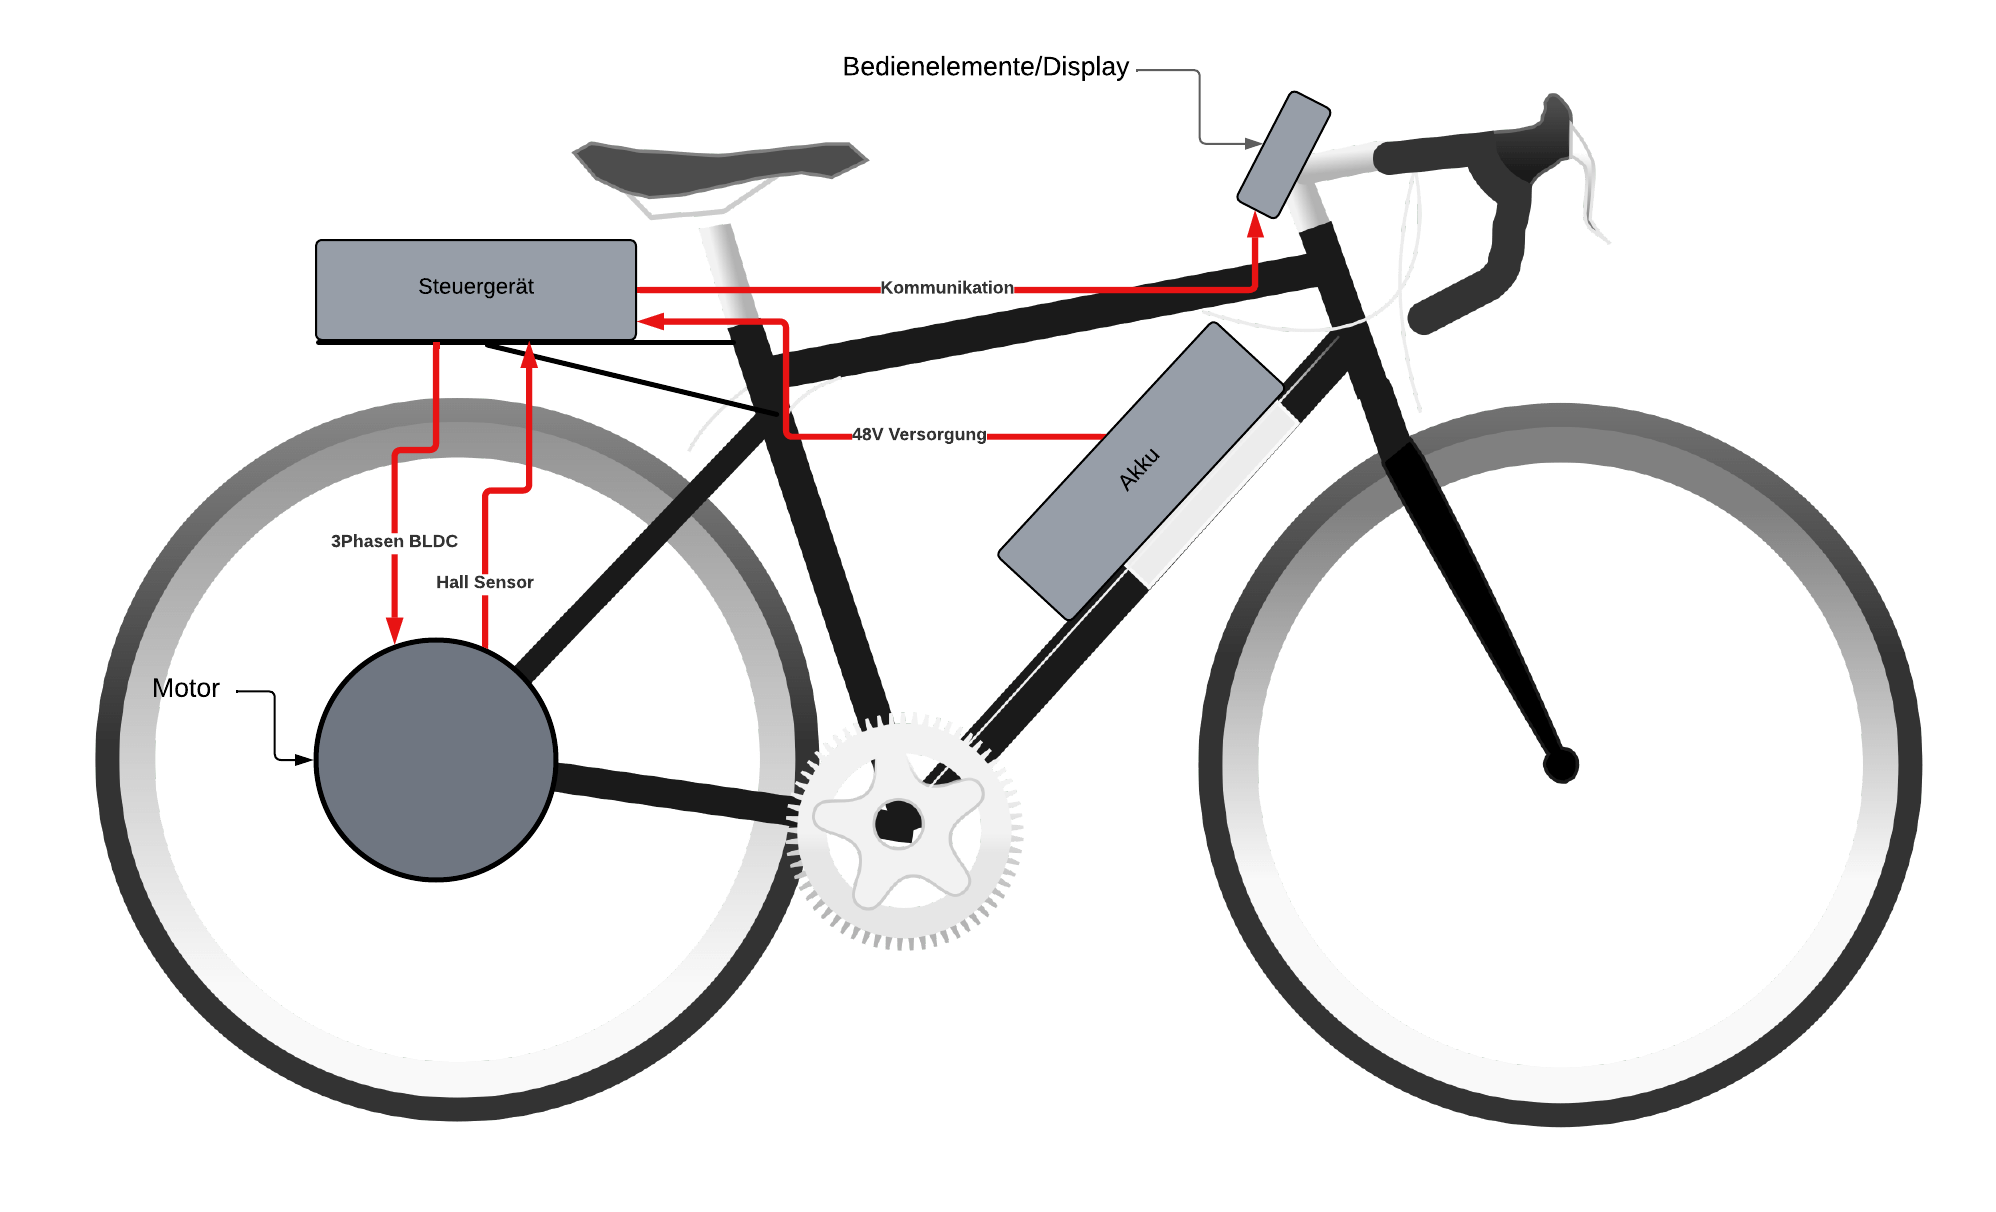
\includegraphics[angle=90,width=12cm]{Bilder/EBike System.PNG}
\caption{Vereinfachtes System Diagramm}
\label{EBike_sys}
\end{center}
\end{figure}


\chapter{Entwicklung}
\begin{figure}[ht]
\begin{center}
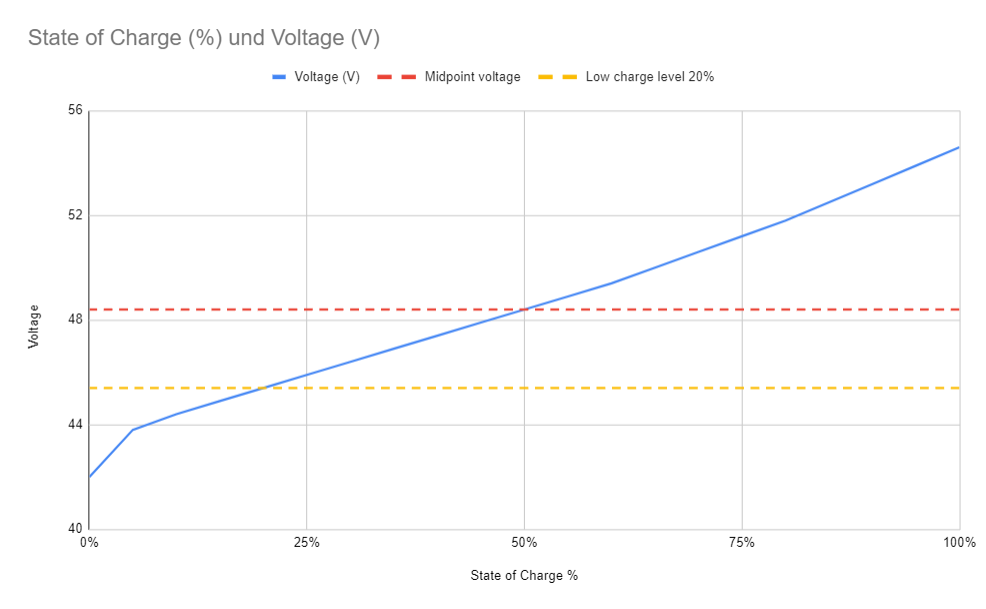
\includegraphics[angle=90,width=14cm]{Bilder/StateofC.PNG}
\caption{48V Akku Spannungskurve}
\label{stateofC}
\end{center}
\end{figure}

\chapter{Schaltplan}
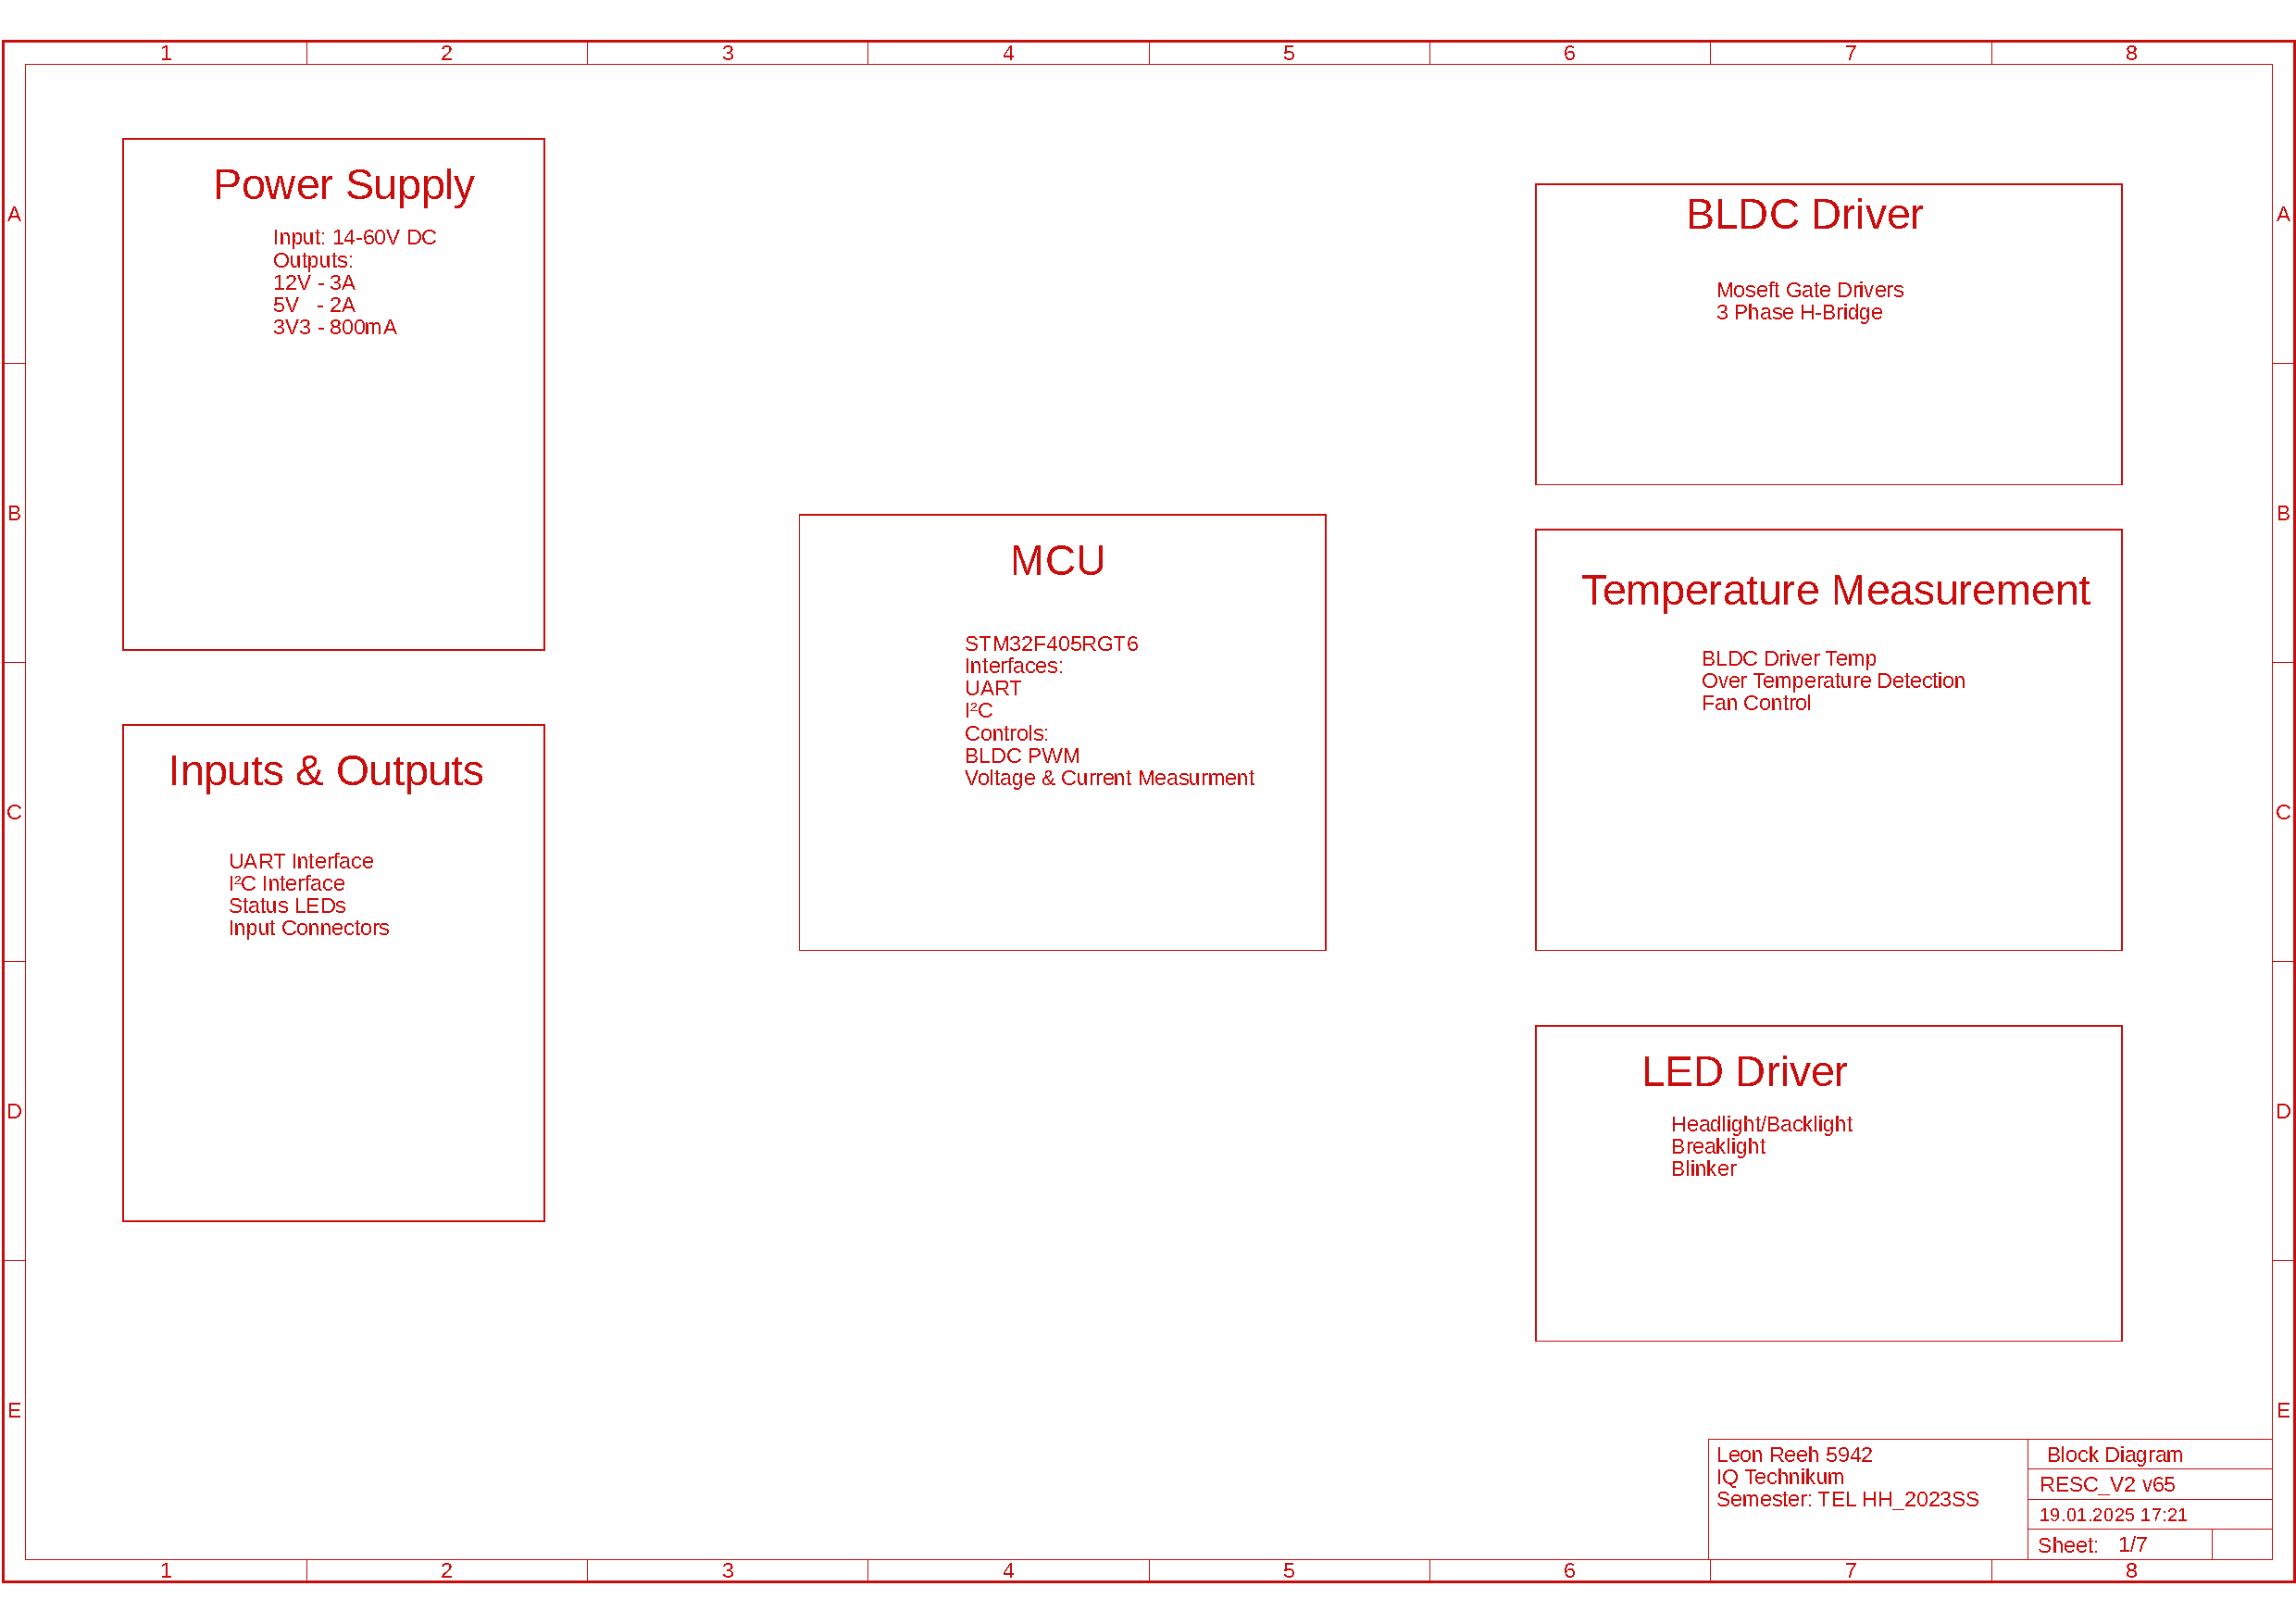
\includepdf[angle=90,pages={1-7}]{PDF/RESC_V2 Schematic.pdf}

\chapter{Layout}
\includepdf[angle=90,pages={1-9}]{PDF/RESC_V2 PCB.pdf}
\chapter{BOM}
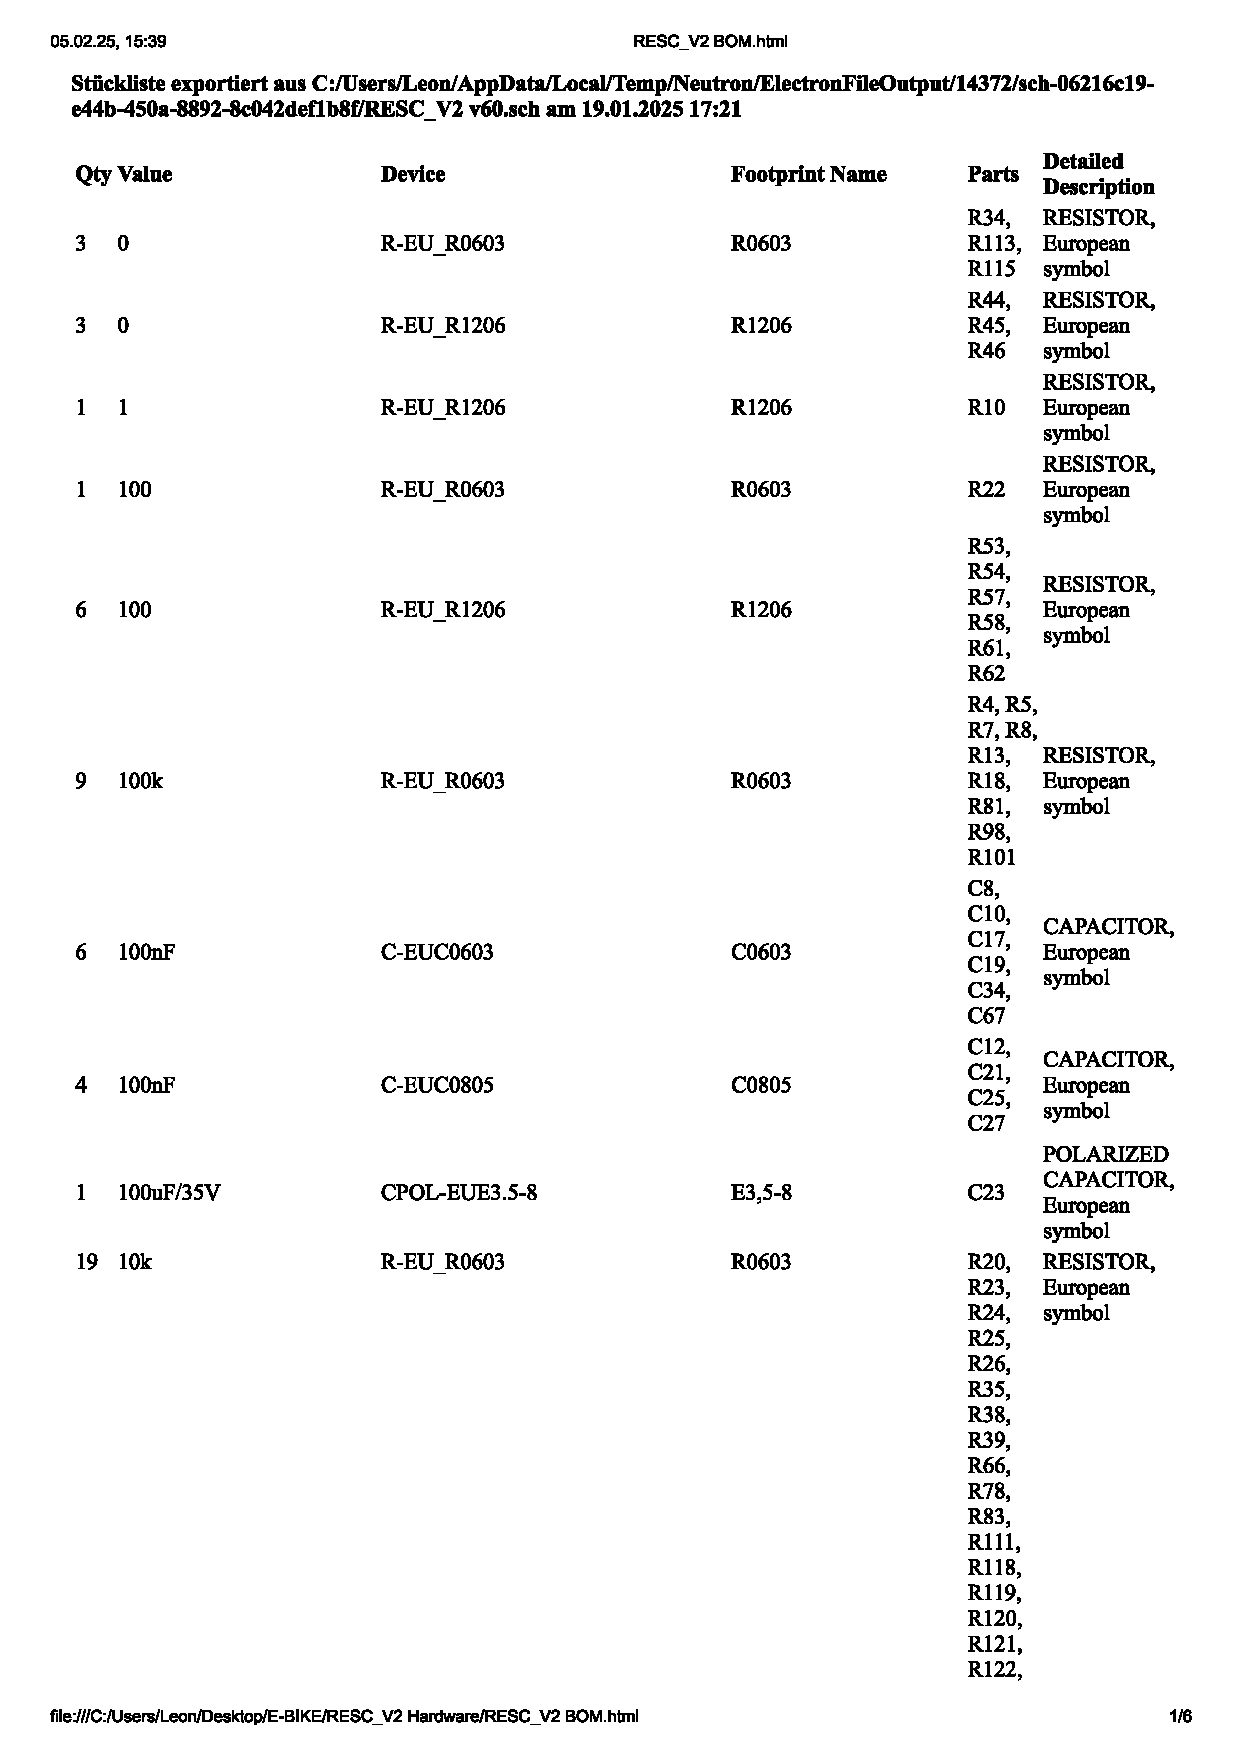
\includepdf[pages={1-6}]{PDF/RESC_V2 BOM.pdf}

\chapter{Source Code}
\section{Main.c/h}
\begin{lstlisting}[language=C, caption=\textbf{Private Defines},label={define}, mathescape=true, breaklines=true]
/* USER CODE BEGIN Private defines */
//Machine States
#define READY 0
#define DRIVE 1
#define BREAK 2
#define SWFAULT 3
#define HWFAULT 4
#define DEBUGST 6
//BLDC
#define THROTTLE_THRESHOLD 30 //Threshold for initial start to prevent adc drift
#define MAXDUTY 100		//Motor PWM Duty Cycle
#define MINDUTY 0		//Motor PWM Duty Cycle
#define MAXADC 3170		//throttle MAX 2,55V
#define MINADC 1055		//throttle MIN 0.85V
#define MAXRPM 4500		//Max RPM of the given motor
#define MINRPM 25		//Min RPM of the given motor
//Software limits for ADC measurments
#define SW_OC 28	//Over Current		28A
#define SW_UV 44	//Under Voltage		44V
#define SW_OV 60	//Over Voltage 		60V
#define SW_OT 100	//Over Temperature 	100C
#define Temp_FAN_ON  80	//Turn on fan here	80C
#define Temp_FAN_OFF 60	//Turn off fan here 60C
//Blinker PWM
#define BLINKER_START 250 // Run blinker at nom. PWM
#define BLINKER_STOP 500  // Turns off blinker PWM
//other
#define ADC_TIMEOUT 20
#define SWFAULT_TIMOUT 300
/* USER CODE END Private defines */
\end{lstlisting}
Die Benutzerdefiniert-Konstanten dienen der Konfiguration von Grenzwerten und Betriebsparametern. Änderungen sind zentral und einfach möglich.
\newpage
\begin{lstlisting}[language=C, caption=\textbf{Main Loop},label={main}, mathescape=true, breaklines=true]
  /* USER CODE BEGIN WHILE */
  while (1)
  {
	  //Read inputs
	  readADCs();
	  readDI();
	  doADCs();
	  /* STATE MACHINE */
	  switch(STATE){
	  	  case READY:
	  		  ready();
	  		  setDO();
	  		  break;
	  	  case DRIVE:
	  		  drive();
	  		  setDO();
	  		  break;
	  	  case BREAK:
	  		  breaking();
	  		  setDO();
	  		  break;
	  	  case SWFAULT:
	  		  resetDO();
	  		  swfault();
	  		  break;
	  	  case HWFAULT:
	  		  resetDO();
	  		  hwfault();
	  		  break;
	  	  case DEBUGST:
	  		  debug();
	  		  setDO();
	  		  break;
	  	  default:
	  		  resetDO();
	  		  hwfault();
	  		  break;
	  	  }
	  //Update LCD every 500ms
	  if(timcc>=5){
		  update_lcd_val(&lcd_val,ADC_VAL);
		  writeState();
		  timcc =0;
	  }
	  HAL_Delay(25);
    /* USER CODE END WHILE */
  }
\end{lstlisting}
Die Endlosschleife (while (1)) ist der zentrale Ablauf des Programms und führt kontinuierlich die Eingabelesung, Zustandsmaschine und die Anzeigeaktualisierung aus.
\newpage
\begin{lstlisting}[language=C, caption=\textbf{void readADCs()},label={readADC}, mathescape=true, breaklines=true]
/**
  * @brief Reads ADC values for voltage, current, and temperature, and updates corresponding variables
  * @param None
  * @retval void
  */
void readADCs(){
	uint16_t a =0;  //Int dump for ADC
	float x = 0.0;
	//READ Voltage
	ADC3_Select_CH(0);
	HAL_ADC_Start(&hadc3);
	HAL_ADC_PollForConversion(&hadc3, ADC_TIMEOUT);
	a =HAL_ADC_GetValue(&hadc3);
	HAL_ADC_Stop(&hadc3);
	x = adc_volt(a);
	ADC_VAL[0] = 0.15 * x + (1.0- 0.05)*ADC_VAL[0];

	//READ Current
	ADC3_Select_CH(1);
	HAL_ADC_Start(&hadc3);
	HAL_ADC_PollForConversion(&hadc3, ADC_TIMEOUT);
	a =HAL_ADC_GetValue(&hadc3);
	HAL_ADC_Stop(&hadc3);
	x = adc_volt(a);
	ADC_VAL[1] = 0.15 * x + (1.0- 0.05)*ADC_VAL[1];

	//READ Temperature
	ADC3_Select_CH(2);
	HAL_ADC_Start(&hadc3);
	HAL_ADC_PollForConversion(&hadc3, ADC_TIMEOUT);
	a =HAL_ADC_GetValue(&hadc3);
	HAL_ADC_Stop(&hadc3);
	x = adc_volt(a);
	ADC_VAL[2] = 0.15 * x + (1.0- 0.05)*ADC_VAL[2];

}
\end{lstlisting}
\newpage
\begin{lstlisting}[language=C, caption=\textbf{void doADCs()},label={doADC}, mathescape=true, breaklines=true]
/**
  * @brief Processes ADC values to monitor and control system states, including fault detection and fan control
  * @param None
  * @retval void
  */
void doADCs() {
    // Ensure ADC_VAL array has enough elements
    if (sizeof(ADC_VAL) / sizeof(ADC_VAL[0]) < 3) {
        // Handle error (e.g., log it, set state to fault)
        STATE = SWFAULT;
        HD44780_SetCursor(0, 1);
        HD44780_PrintStr("ERR:ADC VAL SIZE");
        return;
    }
    // Release SW_FAULT if all conditions are normal
    if (STATE == SWFAULT) {
        if (ADC_VAL[0] < SW_OV && ADC_VAL[0] > SW_UV + 2 &&  // Voltage OK
            ADC_VAL[1] <= 1 &&                              // Current OK
            ADC_VAL[2] <= Temp_FAN_ON) {                    // Temperature OK
            STATE = BREAK;
        }
    }
    // Device is in normal condition
    if (STATE !=SWFAULT){
        // Control the fan based on temperature
        if (ADC_VAL[2] >= Temp_FAN_ON) {
            HAL_GPIO_WritePin(GPIOB, PB8_DO_FAN_Pin, GPIO_PIN_RESET); // FAN ON
        } else if (ADC_VAL[2] <= Temp_FAN_OFF) {
            HAL_GPIO_WritePin(GPIOB, PB8_DO_FAN_Pin, GPIO_PIN_SET);   // FAN OFF
        }
        // Check for software faults and set error messages
        if (ADC_VAL[0] >= SW_OV) {
            setFaultState("ERR:SW OV");
        } else if (ADC_VAL[0] <= SW_UV) {
            setFaultState("ERR:SW UV");
        } else if (ADC_VAL[1] >= SW_OC) {
            setFaultState("ERR:SW OC");
        } else if (ADC_VAL[2] >= SW_OT) {
            setFaultState("ERR:SW OT");
        }
    }
}
\end{lstlisting}
\newpage
\begin{lstlisting}[language=C, caption=\textbf{void readDI()},label={readDI}, mathescape=true, breaklines=true]
/**
  * @brief Reads digital input values from GPIO pins and updates button states
  * @param None
  * @retval void
  */
void readDI(){
    // Button data[Light, Blinker L, Blinker R, Aux]
    uint16_t but_new[4];
    but_new[0] = (GPIOC->IDR & GPIO_IDR_ID10) ? 0x0001 : 0x0000;
    but_new[1] = (GPIOC->IDR & GPIO_IDR_ID11) ? 0x0001 : 0x0000;
    but_new[2] = (GPIOC->IDR & GPIO_IDR_ID12) ? 0x0001 : 0x0000;
    but_new[3] = (GPIOC->IDR & GPIO_IDR_ID13) ? 0x0001 : 0x0000;

    for (int i = 0; i < 4; i++) {
    	but[i] = but_new[i];
        }
}
\end{lstlisting}
\newpage
\begin{lstlisting}[language=C, caption=\textbf{void setDO()},label={setDO}, mathescape=true, breaklines=true]
/**
  * @brief Sets digital output states based on button inputs and updates system behavior accordingly
  * @param None
  * @retval void
  */
void setDO() {
	//Data error
	if (sizeof(but) / sizeof(but[0]) < 4) {
		setFaultState("ERR: DO SIZE");
	}

    // Button data: [Light, Blinker L, Blinker R, Aux]
    // Toggle lights based on button state
    HAL_GPIO_WritePin(GPIOB, PB3_DO_LIGHT_Pin, but[0] == 0 ? GPIO_PIN_RESET : GPIO_PIN_SET);

    // Handle Blinker Left (PWM Control)
    if (but[1] == 1) {
        TIM3->CCR2 = BLINKER_START;  // Start PWM
    } else {
        TIM3->CCR2 = BLINKER_STOP;  // Stop PWM
    }

    // Handle Blinker Right (PWM Control)
    if (but[2] == 1) {
        TIM3->CCR1 = BLINKER_START;  // Start PWM
    } else {
        TIM3->CCR1 = BLINKER_STOP;  // Stop PWM
    }

    // Handle Aux button action
    if (but[3] == 0) {
        HAL_GPIO_TogglePin(PB1_LED_RED_GPIO_Port, PB1_LED_RED_Pin); // Toggle LED
        STATE = DRIVE;                                             // Set state to DRIVE
    }
}
\end{lstlisting}
\newpage
\begin{lstlisting}[language=C, caption=\textbf{void ready()},label={ready}, mathescape=true, breaklines=true]
/**
  * @brief Prepares the system for motor operation by initializing throttle input and PWM control
  * @param None
  * @retval void
  */
void ready() {
    // Start ADC conversion
    HAL_ADC_Start(&hadc1);
    HAL_ADC_PollForConversion(&hadc1, 20);

    // Get throttle raw value
    rawThrot = HAL_ADC_GetValue(&hadc1);

    // Map throttle value to duty cycle range
    int THrotduty = map(rawThrot, MINADC, MAXADC, MINDUTY, MAXDUTY);

    // Check if throttle duty cycle exceeds the threshold
    if (THrotduty >= THROTTLE_THRESHOLD) {
        // Initialize PWM outputs to zero
        TIM1->CCR1 = 0;
        TIM1->CCR2 = 0;
        TIM1->CCR3 = 0;

        // Start PWM for all three channels
        HAL_TIM_PWM_Start(&htim1, TIM_CHANNEL_1);
        HAL_TIM_PWM_Start(&htim1, TIM_CHANNEL_2);
        HAL_TIM_PWM_Start(&htim1, TIM_CHANNEL_3);

        // Initialize BLDC motor
        initBLDC();

        // Set initial duty cycle
        duty = 10; // Set initial duty cycle; modify as needed

        // Change state to DRIVE
        STATE = DRIVE;
    }
}
\end{lstlisting}
\newpage
\begin{lstlisting}[language=C, caption=\textbf{void drive()},label={drive}, mathescape=true, breaklines=true]
/**
  * @brief Controls the motor drive by reading throttle input and updating the PWM duty cycle
  * @param None
  * @retval void
  */
void drive() {
    // Start ADC conversion
    HAL_ADC_Start(&hadc1);

    // Wait for ADC conversion to complete with a timeout
    if (HAL_ADC_PollForConversion(&hadc1, ADC_TIMEOUT) == HAL_OK) {
        // Get raw throttle value
        rawThrot = HAL_ADC_GetValue(&hadc1);

        // Map the raw throttle value to a duty cycle range
        int THrotduty = map(rawThrot, MINADC, MAXADC, MINDUTY, MAXDUTY);

        // Update the duty cycle
        duty = THrotduty;
    } else {
        // Handle ADC conversion error (optional)
        duty = 0; // Set duty to a safe value in case of failure
        setFaultState("ERR: ADC");
        // Optionally log or display an error message
    }
}
\end{lstlisting}
\begin{lstlisting}[language=C, caption=\textbf{void breaking()},label={break}, mathescape=true, breaklines=true]
/**
  * @brief Engages the braking mechanism by stopping PWM outputs and activating braking GPIO pins
  * @param None
  * @retval void
  */
void breaking() {
    // Stop all PWM channels
    TIM1->CCR1 = 0;
    TIM1->CCR2 = 0;
    TIM1->CCR3 = 0;
    duty = 0; // Reset duty cycle to zero

    HAL_TIM_PWM_Stop(&htim1, TIM_CHANNEL_1);
    HAL_TIM_PWM_Stop(&htim1, TIM_CHANNEL_2);
    HAL_TIM_PWM_Stop(&htim1, TIM_CHANNEL_3);

    // Set GPIO pins for braking mode
    HAL_GPIO_WritePin(GPIOB, PB13_U_Pin, GPIO_PIN_SET);
    HAL_GPIO_WritePin(GPIOB, PB14_V_Pin, GPIO_PIN_SET);
    HAL_GPIO_WritePin(GPIOB, PB15_W_Pin, GPIO_PIN_SET);
}
\end{lstlisting}
\newpage
\begin{lstlisting}[language=C, caption=\textbf{void swfault()},label={swfault}, mathescape=true, breaklines=true]
/**
  * @brief Handles the software fault state by engaging braking and transitioning to HWFAULT after a timeout
  * @param None
  * @retval void
  */
void swfault() {
    // Perform breaking to ensure the system is in a safe state
    breaking();

    // Check if the timeout for SWFAULT has elapsed (30s = 300 units of 100ms)
    if (swfault_time_counter >= SWFAULT_TIMOUT) {
        // Transition to HWFAULT state
        STATE = HWFAULT;
    }
}
\end{lstlisting}
\begin{lstlisting}[language=C, caption=\textbf{void hwfault()},label={hwfault}, mathescape=true, breaklines=true]
/**
  * @brief Handles hardware faults by engaging braking, displaying an error message, and halting execution
  * @param None
  * @retval void
  */
void hwfault(){
	STATE = HWFAULT;
	breaking();
	HD44780_SetCursor(0,1);
	HD44780_PrintStr("ERROR:HW FAULT");
	//Stuck untill Power on reset
	while(1){
		HAL_Delay(100);

	}
}
\end{lstlisting}
\newpage
\begin{lstlisting}[language=C, caption=\textbf{void HAL\_GPIO\_EXTI\_Callback(uint16\_t GPIO\_Pin)},label={interrupt}, mathescape=true, breaklines=true]
//Interrupt Pin Function
void HAL_GPIO_EXTI_Callback(uint16_t GPIO_Pin) {
    // Handle Break Signal Interrupt
    if (GPIO_Pin == EXTI5_Break_Pin) {
    	handleBreakInterrupt();
    }
    // Handle Hardware Fault Interrupt
    else if (GPIO_Pin == EXTI9_FAULT_Pin) {
    	handleHardwareFaultInterrupt();
    }
    // Handle Hall Sensor Interrupt
    else if (STATE == DRIVE || STATE == READY) {
        if (GPIO_Pin == EXTI6_HALL_U_Pin || GPIO_Pin == EXTI7_HALL_V_Pin || GPIO_Pin == EXTI8_HALL_W_Pin) {
        	handleHallSensorInterrupt(GPIO_Pin);
        }
    } else {
        // No operation for other states
        __NOP();
    }
}
\end{lstlisting}
\begin{lstlisting}[language=C, caption=\textbf{void handleHardwareFaultInterrupt()},label={hwint}, mathescape=true, breaklines=true]
/**
  * @brief Handles hardware fault interrupts, transitioning motor state to HWFAULT
  * @param None
  * @retval void
  */
void handleHardwareFaultInterrupt() {
	STATE = HWFAULT;
    // Optional: Identify Fault Reason and shutdown Device
    // Example readADCs() and determine fault cause;
}
\end{lstlisting}
\newpage
\begin{lstlisting}[language=C, caption=\textbf{void handleBreakInterrupt()},label={brint}, mathescape=true, breaklines=true]
/**
  * @brief Handles the brake interrupt signal, transitioning motor state between BREAK and READY
  * @param None
  * @retval void
  */
void handleBreakInterrupt() {
    uint16_t breakSignal = (GPIOC->IDR & GPIO_IDR_ID5) ? 0x0001 : 0x0000;
    if (breakSignal == 0) {
        // Transition to BREAK state
        STATE = BREAK;
        HAL_GPIO_WritePin(PB0_LED_GREEN_GPIO_Port, PB0_LED_GREEN_Pin, GPIO_PIN_RESET);
        HAL_GPIO_WritePin(PB1_LED_RED_GPIO_Port, PB1_LED_RED_Pin, GPIO_PIN_SET);
    } else {
        // Transition to READY state if motor is fully stopped
    	if(rpm >=5){
    		STATE = DRIVE;
    	}else{
    		STATE = READY;
    	}
        HAL_GPIO_WritePin(PB0_LED_GREEN_GPIO_Port, PB0_LED_GREEN_Pin, GPIO_PIN_SET);
        HAL_GPIO_WritePin(PB1_LED_RED_GPIO_Port, PB1_LED_RED_Pin, GPIO_PIN_RESET);
    }
}
\end{lstlisting}
\newpage
\begin{lstlisting}[language=C, caption=\textbf{void handleHallSensorInterrupt(uint16\_t GPIO\_Pin)},label={senint}, mathescape=true, breaklines=true]
/**
  * @brief Handles hall sensor interrupts, updates commutator step for motor control
  * @param GPIO_Pin      = Pin number that triggered the interrupt
  * @retval void
  */
void handleHallSensorInterrupt(uint16_t GPIO_Pin) {
    hallCC++; // Increment hall sensor counter

    // Read hall sensor states
    uint16_t hall[3];
    hall[0] = (GPIOC->IDR & GPIO_IDR_ID6) ? 0x0001 : 0x0000; // Sensor U
    hall[1] = (GPIOC->IDR & GPIO_IDR_ID7) ? 0x0001 : 0x0000; // Sensor V
    hall[2] = (GPIOC->IDR & GPIO_IDR_ID8) ? 0x0001 : 0x0000; // Sensor W

    // Trapazoidal control
    uint16_t commutatorStep = hallState(hall);
    commutator(commutatorStep, duty, dir);

    // Optional: Implement sine control as needed
    /*
     * uint16_t commutatorStep = hallState(hall);
     * uint16_t phaseAngle = electricalAngle(commutatorStep);
     * FOCcommutator(phaseAngle, duty);
     */
}

\end{lstlisting}


\newpage
\section{BLDC.c/h}
\begin{lstlisting}[language=C, caption=\textbf{uint16\_t hallState(uint16\_t hall[])},label={hallS}, mathescape=true, breaklines=true]
/**
  * @brief Takes hallsensor states and determines the commutator position
  * @param hall[] 		= arry containing the values read from the 3 Hall Sensors
  * @retval			= The Communator step between 0-5 used to set BLDC gates
  * Hall Sensor State	Rotor Position	Electrical Angle (Degrees)
  *				001		0 - 60			0 - 1440
  *				101		60 - 120		1440 - 2880
  *				100		120 - 180		2880 - 4320
  *				110		180 - 240		4320 - 5760
  *				010		240 - 300		5760 - 7200
  *				011		300 - 360		7200 - 8640
  *
  */
uint16_t hallState(uint16_t hall[]){

	uint16_t commutatorState = -1;
	  if ((hall[0] == 1) && (hall[1] == 0) && (hall[2] == 1)) {
		//Mechanical Angle 0-60
		  commutatorState = 0;
	  }
	  else if  ((hall[0] == 0) && (hall[1] == 0) && (hall[2] == 1)) {
		//Mechanical Angle 60-120
		  commutatorState = 1;
	  }
	  else if  ((hall[0] == 0) && (hall[1] == 1) && (hall[2] == 1)) {
		//Mechanical Angle 120-180
		  commutatorState = 2;
	  }
	  else if  ((hall[0] == 0) && (hall[1] == 1) && (hall[2] == 0)) {
		//Mechanical Angle 180-240
		  commutatorState = 3;
	  }
	  else if  ((hall[0] == 1) && (hall[1] == 1) && (hall[2] == 0)) {
		//Mechanical Angle 240-300
		  commutatorState = 4;
	  }
	  else if  ((hall[0] == 1) && (hall[1] == 0) && (hall[2] == 0)) {
		//Mechanical Angle 300-360
		  commutatorState = 5;
	  }
	  return commutatorState;
}
\end{lstlisting}
\newpage
\begin{lstlisting}[language=C, caption=\textbf{void commutator(int commutatorStep, int duty, int dir)},label={commuta}, mathescape=true, breaklines=true]
/**
  * @brief Sets Three Phase gate driver according to commutator position
  * @param commutatorStep 		= 0-5 determined by FOC hall sensor position
  * @param duty					= PWM duty cycle 0-100
  * @param dir					= motor direction: 1 = fwr; -1= rws
  * @retval			= void
  */
void commutator(int commutatorStep, int duty, int dir){

	if(dir ==1){
		switch(commutatorStep){

		//U PWM
		//Hall state: 		U = HIGH	V = LOW		W = HIGH
		//Phase Current:	U = I		V =	-I		W = 0
		//High Side			U = PWM		V = OFF		W = OFF
		//Low Side			U = OFF		V = ON		W = OFF
		case 0:
			//Low Side
			HAL_GPIO_WritePin(GPIOB,PB13_U_Pin,GPIO_PIN_RESET);
			HAL_GPIO_WritePin(GPIOB,PB14_V_Pin,GPIO_PIN_SET);
			HAL_GPIO_WritePin(GPIOB,PB15_W_Pin,GPIO_PIN_RESET);
			//High Side
			TIM1->CCR1 = duty;
			TIM1->CCR2 = 0;
			TIM1->CCR3 = 0;

			break;

		//W PWM
		//Hall state: 		U = LOW		V = LOW		W = HIGH
		//Phase Current:	U = 0		V =	-I		W = I
		//High Side			U = OFF		V = OFF		W = PWM
		//Low Side			U = OFF		V = ON		W = OFF
		case 1:
			//Low Side
			HAL_GPIO_WritePin(GPIOB,PB13_U_Pin,GPIO_PIN_RESET);
			HAL_GPIO_WritePin(GPIOB,PB14_V_Pin,GPIO_PIN_SET);
			HAL_GPIO_WritePin(GPIOB,PB15_W_Pin,GPIO_PIN_RESET);
			//High Side
			TIM1->CCR1 = 0;
			TIM1->CCR2 = 0;
			TIM1->CCR3 = duty;

			break;

		//W PWM
		//Hall state: 		U = LOW		V = HIGH	W = HIGH
		//Phase Current:	U = -I		V =	0		W = I
		//High Side			U = OFF		V = OFF		W = PWM
		//Low Side			U = ON		V = OFF		W = OFF
		case 2:
			//Low Side
			HAL_GPIO_WritePin(GPIOB,PB13_U_Pin,GPIO_PIN_SET);
			HAL_GPIO_WritePin(GPIOB,PB14_V_Pin,GPIO_PIN_RESET);
			HAL_GPIO_WritePin(GPIOB,PB15_W_Pin,GPIO_PIN_RESET);
			//High Side
			TIM1->CCR1 = 0;
			TIM1->CCR2 = 0;
			TIM1->CCR3 = duty;

			break;

		//V PWM
		//Hall state: 		U = LOW		V = HIGH	W = LOW
		//Phase Current:	U = -I		V =	I		W = 0
		//High Side			U = OFF		V = PWM		W = OFF
		//Low Side			U = ON		V = OFF		W = OFF
		case 3:
			//Low Side
			HAL_GPIO_WritePin(GPIOB,PB13_U_Pin,GPIO_PIN_SET);
			HAL_GPIO_WritePin(GPIOB,PB14_V_Pin,GPIO_PIN_RESET);
			HAL_GPIO_WritePin(GPIOB,PB15_W_Pin,GPIO_PIN_RESET);
			//High Side
			TIM1->CCR1 = 0;
			TIM1->CCR2 = duty;
			TIM1->CCR3 = 0;

			break;

		//V PWM
		//Hall state: 		U = HIGH; 	V = HIGH	W = LOW
		//Phase Current:	U = 0		V =	I		W = -I
		//High Side			U = OFF		V = PWM		W = OFF
		//Low Side			U = OFF		V = OFF		W = ON
		case 4:
			//Low Side
			HAL_GPIO_WritePin(GPIOB,PB13_U_Pin,GPIO_PIN_RESET);
			HAL_GPIO_WritePin(GPIOB,PB14_V_Pin,GPIO_PIN_RESET);
			HAL_GPIO_WritePin(GPIOB,PB15_W_Pin,GPIO_PIN_SET);
			//High Side
			TIM1->CCR1 = 0;
			TIM1->CCR2 = duty;
			TIM1->CCR3 = 0;

			break;

		//U PWM
		//Hall state: 		U = HIGH	V = LOW		W = LOW
		//Phase Current:	U = I		V =	0		W = -I
		//High Side			U = PWM		V = OFF		W = OFF
		//Low Side			U = OFF		V = OFF		W = ON
		case 5:
			//Low Side
			HAL_GPIO_WritePin(GPIOB,PB13_U_Pin,GPIO_PIN_RESET);
			HAL_GPIO_WritePin(GPIOB,PB14_V_Pin,GPIO_PIN_RESET);
			HAL_GPIO_WritePin(GPIOB,PB15_W_Pin,GPIO_PIN_SET);
			//High Side
			TIM1->CCR1 = duty;
			TIM1->CCR2 = 0;
			TIM1->CCR3 = 0;

			break;

		//i have no idea how you ended up here pls stop motor
		//High Side			U = OFF		V = OFF		W = OFF
		//Low Side			U = HIGH	V = HIGH	W = HIGH
		default:
			HAL_GPIO_WritePin(GPIOB,PB13_U_Pin,GPIO_PIN_SET);
			HAL_GPIO_WritePin(GPIOB,PB14_V_Pin,GPIO_PIN_SET);
			HAL_GPIO_WritePin(GPIOB,PB15_W_Pin,GPIO_PIN_SET);

			TIM1->CCR1 = 0;
			TIM1->CCR2 = 0;
			TIM1->CCR3 = 0;
			break;
		}
	}
	if(dir !=1){
		//no implimentation for reverse needed yet just break
		HAL_GPIO_WritePin(GPIOB,PB13_U_Pin,GPIO_PIN_SET);
		HAL_GPIO_WritePin(GPIOB,PB14_V_Pin,GPIO_PIN_SET);
		HAL_GPIO_WritePin(GPIOB,PB15_W_Pin,GPIO_PIN_SET);

		TIM1->CCR1 = 0;
		TIM1->CCR2 = 0;
		TIM1->CCR3 = 0;
	}
}
\end{lstlisting}
\newpage
\begin{lstlisting}[language=C, caption=\textbf{void initBLDC()},label={initBL}, mathescape=true, breaklines=true]
/**
  * @brief Initializes the BLDC motor by reading hall sensor values and setting the commutator step
  * @param None
  * @retval void
  */
void initBLDC(){
	uint16_t hall[3];
	hall[0]= (GPIOC->IDR & GPIO_IDR_ID6)? 0x0001 : 0x0000; // Sensor A
	hall[1]= (GPIOC->IDR & GPIO_IDR_ID7)? 0x0001 : 0x0000; // Sensor B
	hall[2]= (GPIOC->IDR & GPIO_IDR_ID8)? 0x0001 : 0x0000; // Sensor C

	int step= hallState(hall);
	commutator(step, 15,1);
}

\end{lstlisting}

\begin{lstlisting}[language=C, caption=\textbf{void BLDCbreak()},label={BLbreak}, mathescape=true, breaklines=true]
/**
  * @brief Engages the brake for the BLDC motor by setting all output phases high and stopping PWM signals
  * @param None
  * @retval void
  */
void BLDCbreak(){
	HAL_GPIO_WritePin(GPIOB,PB13_U_Pin,GPIO_PIN_SET);
	HAL_GPIO_WritePin(GPIOB,PB14_V_Pin,GPIO_PIN_SET);
	HAL_GPIO_WritePin(GPIOB,PB15_W_Pin,GPIO_PIN_SET);

	TIM1->CCR1 = 0;
	TIM1->CCR2 = 0;
	TIM1->CCR3 = 0;
}
\end{lstlisting}
\newpage
\section{liquidcrystal\_i2c.c/h}
\begin{lstlisting}[language=C, caption=\textbf{lcd struct},label={struct},mathescape=true, breaklines=true] 
/* lcd stuct */
typedef struct{
//Values for updating the display
  char volt[4] /*Storage DC Voltage */;
  char temp[3] /*Storage Drive temperature*/;
  char amp[4] /*Storage DC Current*/;
  char speed[2] /*Storage bike Speed*/;
  char erpm[4] /*Storage Motor rpm*/;
  char pwm[2] /*Storage PWM value*/;

//Cursor position for respective Values
  uint8_t cur_volt[2];
  uint8_t cur_temp[2];
  uint8_t cur_amp[2];
  uint8_t cur_speed[2];
  uint8_t cur_erpm[2];
  uint8_t cur_pwm[2];
} lcd_ar;
\end{lstlisting}

\begin{lstlisting}[language=C, caption=\textbf{void HD44780\_SetCursor(uint8\_t col, uint8\_t row)},label={setC}, mathescape=true, breaklines=true]
/**
  * @brief Sets the cursor position on the HD44780 LCD display
  * @param col    = Column position (0-based)
  * @param row    = Row position (0-based)
  * @retval void
  */
void HD44780_SetCursor(uint8_t col, uint8_t row)
{
  int row_offsets[] = { 0x00, 0x40, 0x14, 0x54 };
  if (row >= dpRows)
  {
    row = dpRows-1;
  }
  SendCommand(LCD_SETDDRAMADDR | (col + row_offsets[row]));
}
\end{lstlisting}

\begin{lstlisting}[language=C, caption=\textbf{void HD44780\_PrintStr(const char c[])},label={print}, mathescape=true, breaklines=true]
/**
  * @brief Prints a string to the HD44780 LCD display
  * @param c    = Pointer to a null-terminated string to display
  * @retval void
  */
void HD44780_PrintStr(const char c[])
{
  while(*c) SendChar(*c++);
}
\end{lstlisting}

\begin{lstlisting}[language=C, caption=\textbf{void Init\_lcd\_ar(lcd\_ar* lcd)},label={initLCD}, mathescape=true, breaklines=true]
/**
  * @brief Initializes the lcd_ar struct with default cursor positions and display values
  * @param lcd    = Pointer to an lcd_ar struct to initialize
  * @retval void
  */
void Init_lcd_ar(lcd_ar* lcd){
	//Load cursor positions
	lcd ->cur_volt[0] =15;
	lcd ->cur_volt[1] =0;

	lcd ->cur_temp[0]=0;
	lcd ->cur_temp[1]=0;

	lcd ->cur_amp[0] =15;
	lcd ->cur_amp[1] =1;

	lcd ->cur_speed[0]=9;
	lcd ->cur_speed[1]=3;

	lcd ->cur_erpm[0]=0;
	lcd ->cur_erpm[1]=3;

	lcd ->cur_pwm[0]=1;
	lcd ->cur_pwm[1]=2;

	//Set up Display for array mode
	//Init Volt
	HD44780_SetCursor(15,0);
	HD44780_PrintStr("42.0V");
	//Init Temp
	HD44780_SetCursor(0,0);
	HD44780_PrintStr("069C");
	//Init Current
	HD44780_SetCursor(15,1);
	HD44780_PrintStr("02.5A");
	//Init Speed
	HD44780_SetCursor(9,3);
	HD44780_PrintStr("10KM/H");
	//Init ERPM
	HD44780_SetCursor(0,3);
	HD44780_PrintStr("4000");
	//Iinit PWM
	//HD44780_SetCursor(1,2);
	//HD44780_PrintStr("00%");
}
\end{lstlisting}
\newpage
\begin{lstlisting}[language=C, caption=\textbf{void update\_lcd\_val(lcd\_ar* ar, float val[])},label={upLCD}, mathescape=true, breaklines=true]
/**
  * @brief Updates the lcd_ar struct and LCD display with new sensor values
  * @param ar     = Pointer to an lcd_ar struct containing cursor positions
  * @param val    = Array of float values to update [Voltage, Current, Temperature, Speed, (optional: PWM)]
  * @retval void
  */
void update_lcd_val(lcd_ar* ar, float val[]){
	//Set Voltage
	snprintf(ar->volt, 5, "%04.1f", val[0]);
	HD44780_SetCursor(ar->cur_volt[0],ar->cur_volt[1]);
	HD44780_PrintStr(ar->volt);
	//Set Current
	snprintf(ar->amp, 5, "%04.1f", val[1]);
	HD44780_SetCursor(ar->cur_amp[0],ar->cur_amp[1]);
	HD44780_PrintStr(ar->amp);
	//Set Temp
	snprintf(ar->temp, 4, "%03.0f", val[2]);
	HD44780_SetCursor(ar->cur_temp[0],ar->cur_temp[1]);
	HD44780_PrintStr(ar->temp);
	//Set Speed
	snprintf(ar->speed, 3, "%02.0f",val[3] );
	HD44780_SetCursor(ar->cur_speed[0],ar->cur_speed[1]);
	HD44780_PrintStr(ar->speed);
	//Set ERPM
	snprintf(ar->erpm, 5, "%04.0f",rpm);
	HD44780_SetCursor(ar->cur_erpm[0],ar->cur_erpm[1]);
	HD44780_PrintStr(ar->erpm);
	//Set PWm
	//snprintf(ar->pwm,3,"%02.0f",val[4] );
	//HD44780_SetCursor(ar->cur_pwm[0],ar->cur_pwm[1]);
	//HD44780_PrintStr(ar->pwm);

}
\end{lstlisting}
\newpage
\section{Mymath.c/h}
\begin{lstlisting}[language=C, caption=\textbf{pid struct},label={pid}, mathescape=true, breaklines=true]
typedef struct{
  float max /*! Max manipulated value */;
  float min /*! Miniumum manipulated value */;
  float e /*! Error value */;
  float i /*! Integrator value */;
  float kp /*! Proportional constant */;
  float ki /*! Integrator constant */;
  float kd /*! Differential constant */;
} pid_f_t;
\end{lstlisting}

\begin{lstlisting}[language=C, caption=\textbf{uint16\_t map()},label={map}, mathescape=true, breaklines=true]
/**
  * @brief Re-maps a number from one range to another
  * @param x 		= The number to map.
  * @param in_min	= The lower bound of the values current range.
  * @param in_max	= The upper bound of the values current range.
  * @param out_min	= The lower bound of the values target range.
  * @param out_max	= The upper bound of the values target range.
  * @retval			= The mapped value
  */
uint16_t map(uint16_t x, uint16_t in_min, uint16_t in_max, uint16_t out_min, uint16_t out_max) {
  return (x - in_min) * (out_max - out_min) / (in_max - in_min) + out_min;
}
\end{lstlisting}

\begin{lstlisting}[language=C, caption=\textbf{float adc\_volt(uint16\_t val)},label={adcV}, mathescape=true, breaklines=true]
/**
  * @brief Converts a raw ADC value to the corresponding input voltage
  * @param val    = Raw 12-bit ADC value (0-4095)
  * @retval float = Calculated input voltage
  */
float adc_volt(uint16_t val){
	//((val/(39000+2200))*2200) /12bitADC
    float Vcc = 3.3;
    float R1 = 37000.0;
    float R2 = 2200.0;
    // Convert ADC value to voltage across R2
    float Vout = (val / 4095.0) * Vcc;

    // Calculate the total voltage across R1 and R2
    float Vin = Vout * (R1 + R2) / R2;

    return Vin;
}
\end{lstlisting}
\newpage
\begin{lstlisting}[language=C, caption=\textbf{float adc\_cur(uint16\_t val)},label={adcC}, mathescape=true, breaklines=true]
/**
  * @brief Converts a raw ADC value to the corresponding current based on shunt resistor and amplification factor
  * @param val    = Raw 12-bit ADC value (0-4095)
  * @retval float = Calculated current in amperes
  */
float adc_cur(uint16_t val){
    float Vcc = 3.3;
    float amplification_factor = 20.0;
    float R_shunt = 0.004;
    float offset_voltage = Vcc / 2.0;

    // Convert ADC value to the amplified voltage
    float Vadc = (val / 4095.0) * Vcc;

    // Adjust for the offset voltage
    float Vadc_adjusted = Vadc - offset_voltage;

    // Determine the actual voltage drop across the shunt
    float Vshunt = Vadc_adjusted / amplification_factor;

    // Calculate the current through the shunt
    float current = Vshunt / R_shunt;
    return current;
}
\end{lstlisting}

\begin{lstlisting}[language=C, caption=\textbf{float adc\_temp(uint16\_t val)},label={adcT}, mathescape=true, breaklines=true]
/**
  * @brief Converts a raw ADC value to the corresponding temperature in Celsius using an NTC thermistor
  * @param val    = Raw 12-bit ADC value (0-4095)
  * @retval float = Calculated temperature in Celsius
  */
float adc_temp(uint16_t val){
    float Vcc = 3.3;
    float R2 = 10000.0;
    float T0 = 298.15; // 25C in Kelvin
    float R0 = 10000.0; // Resistance at 25C
    float B = 2904.0; // Beta parameter

    // Convert ADC value to voltage
    float Vadc = (val / 4095.0) * Vcc;

    // Calculate the resistance of the NTC thermistor
    float R1 = R2 * (Vcc / Vadc - 1.0);
    // Calculate temperature in Kelvin using B-parameter equation
    float T = 1.0 / ((1.0 / T0) + (1.0 / B) * log(R1 / R0));
    // Convert Kelvin to Celsius
    float T_Celsius = T - 273.15;
    return T_Celsius;
}
\end{lstlisting}

\begin{lstlisting}[language=C, caption=\textbf{float rpm\_tokmh(float rpm)},label={kmh}, mathescape=true, breaklines=true]
/**
  * @brief Converts motor RPM to speed in kilometers per hour (km/h) based on wheel circumference
  * @param rpm    = Motor RPM (revolutions per minute)
  * @retval float = Calculated speed in kilometers per hour (km/h)
  */
float rpm_tokmh(float rpm){
	//36inch wheel
	//91,44 cm wheel
	//U = 2*pi*r
	//U = 287,267cm
	//U = 2,87267m
	float circumference = 2.87267;
    // distance traveled per minute in meters
    float distance_per_minute = rpm * circumference;
    // Convert distance to kilometers per hour
    float speed_kmh = distance_per_minute * 60 / 1000;
    return speed_kmh;
}
\end{lstlisting}

\section{stm32f4xx\_it.c/h}
\begin{lstlisting}[language=C, caption=\textbf{void TIM2\_IRQHandler(void)},label={tim2}, mathescape=true, breaklines=true]
/**
  * @brief This function handles TIM2 global interrupt.
  */
void TIM2_IRQHandler(void)
{
	int x = hallCC*10;
	float rev = x/24;
	rpm = rev*60;
	hallCC = 0;
	ADC_VAL[3] = rpm_tokmh(rpm);
	//HAL_GPIO_TogglePin(PB1_LED_RED_GPIO_Port,PB1_LED_RED_Pin);
	if(timcc >= 10){
		timcc = 0;
	}else{
		timcc++;
	}
	 // Increment counter only if in SWFAULT state
	if (STATE == SWFAULT) {
		swfault_time_counter++;
	} else {
		// Reset the counter if leaving SWFAULT state
        swfault_time_counter = 0;
	}
  HAL_TIM_IRQHandler(&htim2);
}
\end{lstlisting}





\chapter{Quellen}
Vedder, B. (2019). VESC 4.12 Open Source BLDC ESC. VESC-Project.\\
C2000 Systems and Applications Team, Akin, B., Bhardwaj, M., \& Warriner, J. (2015). Trapezoidal Control of BLDC Motors Using Hall Effect Sensors. Texas Instruments.\\
Hein, M. (2020). Demystifying BLDC motor commutation: Trap, Sine, \& FOC. Texas Instruments.\\
Abacan, A. (2020). Sensored 3-Phase BLDC Motor Control Using Sinusoidal Drive. MicroChip.\\
Simple Projects. (2017). Sensored brushless DC motor control. Simple Circuits.\\
Stratify Labs. (2013). Motor Control using PWM and PID. Stratify Labs.\\
\section{Danksagungen}
Dieses Projekt wurde durch mehrere Ressourcen inspiriert und unterstützt.
Ein besonderer Dank gilt allen Mitwirkenden und der Open-Source-Community für ihre wertvollen Ressourcen und ihre Unterstützung.

\end{document}
